\documentclass[]{article}
\usepackage{lmodern}
\usepackage{amssymb,amsmath}
\usepackage{ifxetex,ifluatex}
\usepackage{fixltx2e} % provides \textsubscript
\ifnum 0\ifxetex 1\fi\ifluatex 1\fi=0 % if pdftex
  \usepackage[T1]{fontenc}
  \usepackage[utf8]{inputenc}
\else % if luatex or xelatex
  \ifxetex
    \usepackage{mathspec}
  \else
    \usepackage{fontspec}
  \fi
  \defaultfontfeatures{Ligatures=TeX,Scale=MatchLowercase}
\fi
% use upquote if available, for straight quotes in verbatim environments
\IfFileExists{upquote.sty}{\usepackage{upquote}}{}
% use microtype if available
\IfFileExists{microtype.sty}{%
\usepackage{microtype}
\UseMicrotypeSet[protrusion]{basicmath} % disable protrusion for tt fonts
}{}
\usepackage[margin=1in]{geometry}
\usepackage{hyperref}
\hypersetup{unicode=true,
            pdftitle={Statistik mit R für Fortgeschrittene},
            pdfauthor={Walter Gruber},
            pdfborder={0 0 0},
            breaklinks=true}
\urlstyle{same}  % don't use monospace font for urls
\usepackage{color}
\usepackage{fancyvrb}
\newcommand{\VerbBar}{|}
\newcommand{\VERB}{\Verb[commandchars=\\\{\}]}
\DefineVerbatimEnvironment{Highlighting}{Verbatim}{commandchars=\\\{\}}
% Add ',fontsize=\small' for more characters per line
\usepackage{framed}
\definecolor{shadecolor}{RGB}{248,248,248}
\newenvironment{Shaded}{\begin{snugshade}}{\end{snugshade}}
\newcommand{\AlertTok}[1]{\textcolor[rgb]{0.94,0.16,0.16}{#1}}
\newcommand{\AnnotationTok}[1]{\textcolor[rgb]{0.56,0.35,0.01}{\textbf{\textit{#1}}}}
\newcommand{\AttributeTok}[1]{\textcolor[rgb]{0.77,0.63,0.00}{#1}}
\newcommand{\BaseNTok}[1]{\textcolor[rgb]{0.00,0.00,0.81}{#1}}
\newcommand{\BuiltInTok}[1]{#1}
\newcommand{\CharTok}[1]{\textcolor[rgb]{0.31,0.60,0.02}{#1}}
\newcommand{\CommentTok}[1]{\textcolor[rgb]{0.56,0.35,0.01}{\textit{#1}}}
\newcommand{\CommentVarTok}[1]{\textcolor[rgb]{0.56,0.35,0.01}{\textbf{\textit{#1}}}}
\newcommand{\ConstantTok}[1]{\textcolor[rgb]{0.00,0.00,0.00}{#1}}
\newcommand{\ControlFlowTok}[1]{\textcolor[rgb]{0.13,0.29,0.53}{\textbf{#1}}}
\newcommand{\DataTypeTok}[1]{\textcolor[rgb]{0.13,0.29,0.53}{#1}}
\newcommand{\DecValTok}[1]{\textcolor[rgb]{0.00,0.00,0.81}{#1}}
\newcommand{\DocumentationTok}[1]{\textcolor[rgb]{0.56,0.35,0.01}{\textbf{\textit{#1}}}}
\newcommand{\ErrorTok}[1]{\textcolor[rgb]{0.64,0.00,0.00}{\textbf{#1}}}
\newcommand{\ExtensionTok}[1]{#1}
\newcommand{\FloatTok}[1]{\textcolor[rgb]{0.00,0.00,0.81}{#1}}
\newcommand{\FunctionTok}[1]{\textcolor[rgb]{0.00,0.00,0.00}{#1}}
\newcommand{\ImportTok}[1]{#1}
\newcommand{\InformationTok}[1]{\textcolor[rgb]{0.56,0.35,0.01}{\textbf{\textit{#1}}}}
\newcommand{\KeywordTok}[1]{\textcolor[rgb]{0.13,0.29,0.53}{\textbf{#1}}}
\newcommand{\NormalTok}[1]{#1}
\newcommand{\OperatorTok}[1]{\textcolor[rgb]{0.81,0.36,0.00}{\textbf{#1}}}
\newcommand{\OtherTok}[1]{\textcolor[rgb]{0.56,0.35,0.01}{#1}}
\newcommand{\PreprocessorTok}[1]{\textcolor[rgb]{0.56,0.35,0.01}{\textit{#1}}}
\newcommand{\RegionMarkerTok}[1]{#1}
\newcommand{\SpecialCharTok}[1]{\textcolor[rgb]{0.00,0.00,0.00}{#1}}
\newcommand{\SpecialStringTok}[1]{\textcolor[rgb]{0.31,0.60,0.02}{#1}}
\newcommand{\StringTok}[1]{\textcolor[rgb]{0.31,0.60,0.02}{#1}}
\newcommand{\VariableTok}[1]{\textcolor[rgb]{0.00,0.00,0.00}{#1}}
\newcommand{\VerbatimStringTok}[1]{\textcolor[rgb]{0.31,0.60,0.02}{#1}}
\newcommand{\WarningTok}[1]{\textcolor[rgb]{0.56,0.35,0.01}{\textbf{\textit{#1}}}}
\usepackage{longtable,booktabs}
\usepackage{graphicx,grffile}
\makeatletter
\def\maxwidth{\ifdim\Gin@nat@width>\linewidth\linewidth\else\Gin@nat@width\fi}
\def\maxheight{\ifdim\Gin@nat@height>\textheight\textheight\else\Gin@nat@height\fi}
\makeatother
% Scale images if necessary, so that they will not overflow the page
% margins by default, and it is still possible to overwrite the defaults
% using explicit options in \includegraphics[width, height, ...]{}
\setkeys{Gin}{width=\maxwidth,height=\maxheight,keepaspectratio}
\IfFileExists{parskip.sty}{%
\usepackage{parskip}
}{% else
\setlength{\parindent}{0pt}
\setlength{\parskip}{6pt plus 2pt minus 1pt}
}
\setlength{\emergencystretch}{3em}  % prevent overfull lines
\providecommand{\tightlist}{%
  \setlength{\itemsep}{0pt}\setlength{\parskip}{0pt}}
\setcounter{secnumdepth}{5}
% Redefines (sub)paragraphs to behave more like sections
\ifx\paragraph\undefined\else
\let\oldparagraph\paragraph
\renewcommand{\paragraph}[1]{\oldparagraph{#1}\mbox{}}
\fi
\ifx\subparagraph\undefined\else
\let\oldsubparagraph\subparagraph
\renewcommand{\subparagraph}[1]{\oldsubparagraph{#1}\mbox{}}
\fi

%%% Use protect on footnotes to avoid problems with footnotes in titles
\let\rmarkdownfootnote\footnote%
\def\footnote{\protect\rmarkdownfootnote}

%%% Change title format to be more compact
\usepackage{titling}

% Create subtitle command for use in maketitle
\providecommand{\subtitle}[1]{
  \posttitle{
    \begin{center}\large#1\end{center}
    }
}

\setlength{\droptitle}{-2em}

  \title{Statistik mit R für Fortgeschrittene}
    \pretitle{\vspace{\droptitle}\centering\huge}
  \posttitle{\par}
    \author{Walter Gruber}
    \preauthor{\centering\large\emph}
  \postauthor{\par}
      \predate{\centering\large\emph}
  \postdate{\par}
    \date{2019-04-15}


\begin{document}
\maketitle

{
\setcounter{tocdepth}{2}
\tableofcontents
}
\hypertarget{section}{%
\section*{}\label{section}}
\addcontentsline{toc}{section}{}

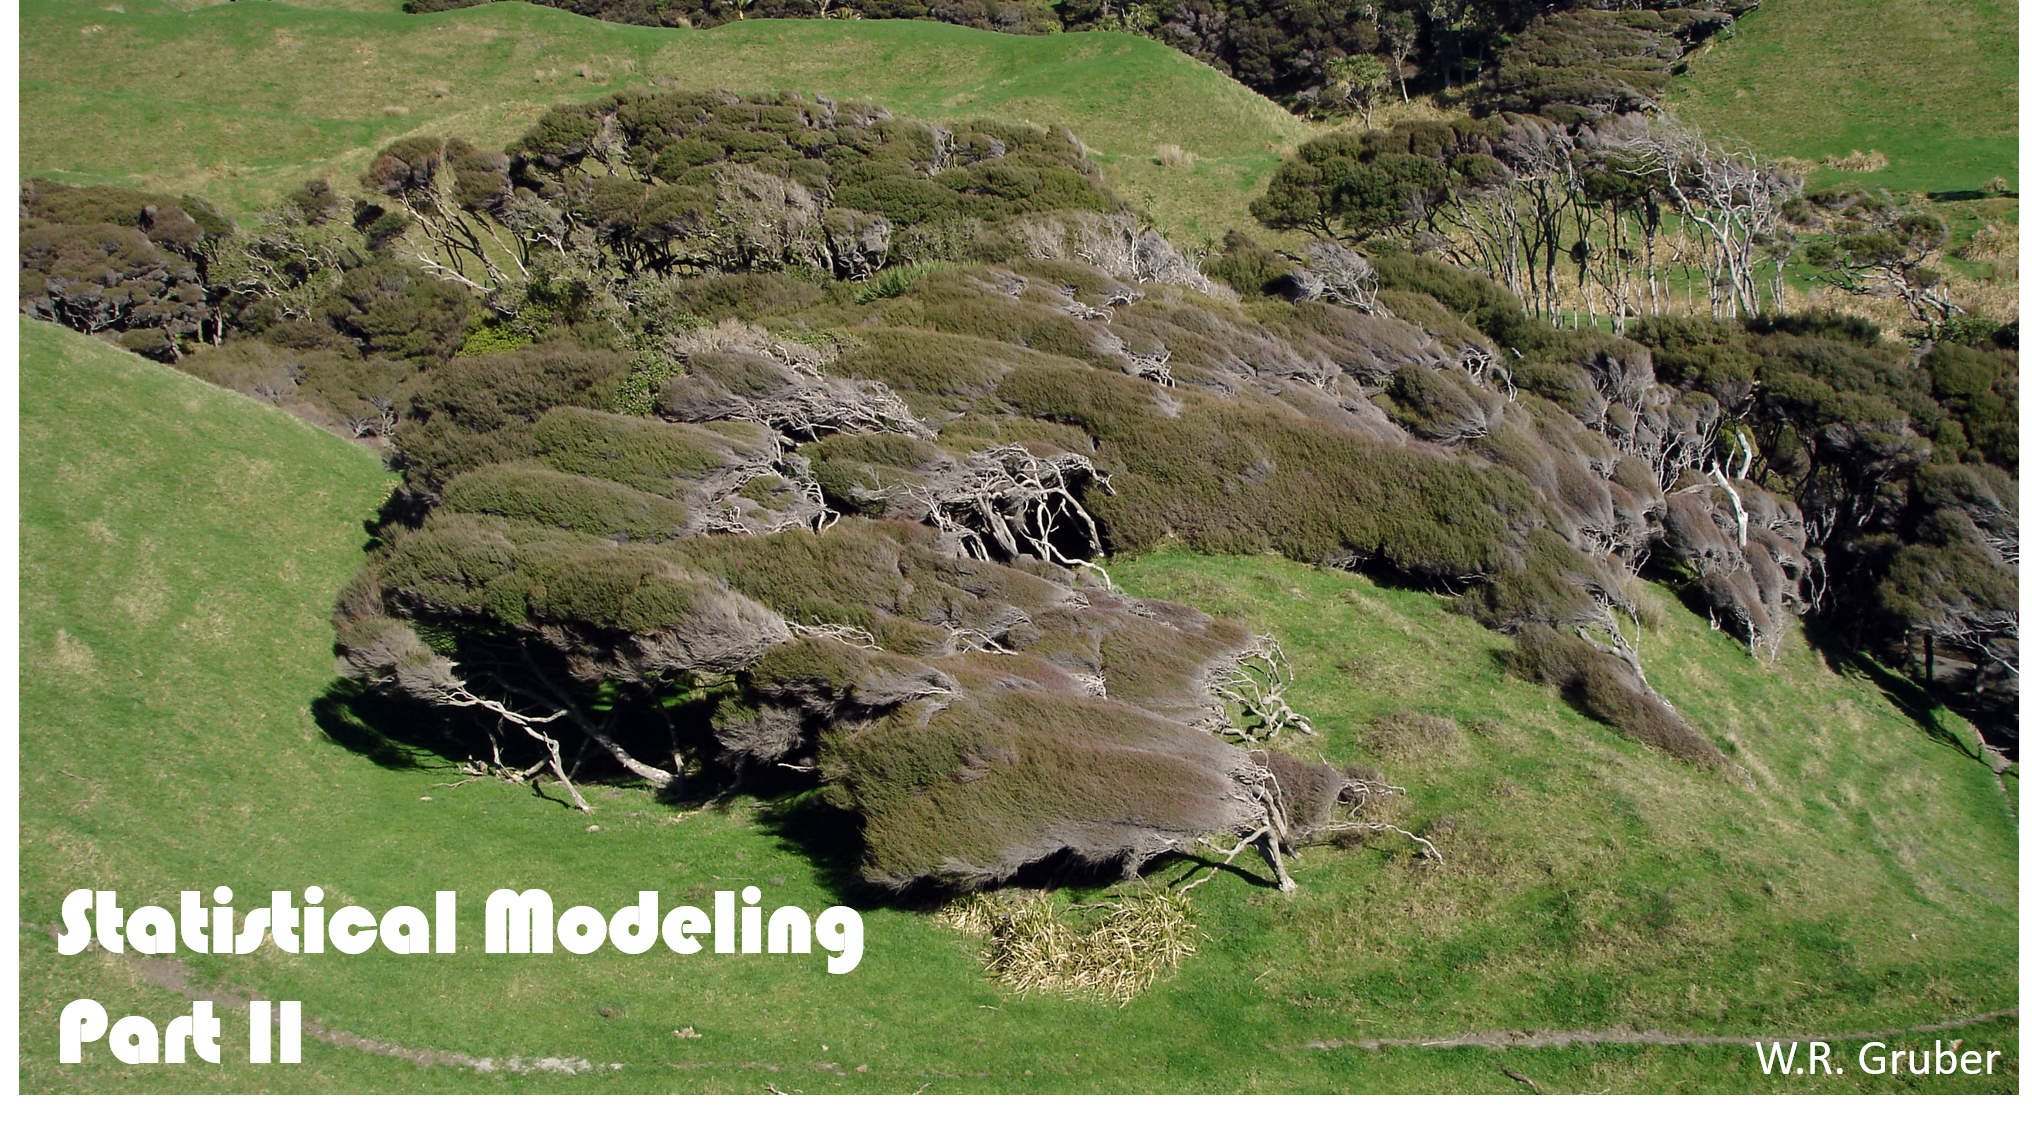
\includegraphics[width=1\textwidth,height=\textheight]{Images/Cover.png}

\hypertarget{vorbemerkung}{%
\section*{Vorbemerkung}\label{vorbemerkung}}
\addcontentsline{toc}{section}{Vorbemerkung}

Dieses Skriptum wurde mit dem Paket \emph{bookdown} erstellt. Der verwendete R-Code wird als Teil des Skriptums angeführt und kann auch direkt von diesem Dokument in ein R-Skript übernommen und ausgeführt werden. Erläuterungen zum Code beschränken sich zum Teil auf wesentliche Code-Fragmente. Für detaillierte Angaben zu diversen Funktionen ist die R-Hilfe zu verwenden.

Der nachfolgende Code ist spezifisch für die Erstellung dieses Dokumentes, sowie der Bearbeitung der Beispiele im Kurs von Bedeutung. Es wird in diesem Code-Teil sichergestellt, dass die verwendeten Pakte vorhanden und geladen sind. Daher sollte dieser Code am Anfang jeder neuen R-Datei übernommen werden. Die Vorgehensweise ist:

\begin{enumerate}
\def\labelenumi{\arabic{enumi}.}
\tightlist
\item
  Starten von R-Studio
\item
  Öffnen einer neuen R-Script Datei
\item
  Kopiere die nachfolgenden Zeilen in diese Datei
\item
  Speichere die Datei mit einem entsprechenden Namen
\item
  Führe diesen Code aus
\item
  Füge deinen Code nach diesen Zeilen ein
\end{enumerate}

\begin{Shaded}
\begin{Highlighting}[]
\CommentTok{# Initialisierung}
\KeywordTok{rm}\NormalTok{(}\DataTypeTok{list =} \KeywordTok{ls}\NormalTok{())}
\ControlFlowTok{if}\NormalTok{ (}\OperatorTok{!}\KeywordTok{require}\NormalTok{(}\StringTok{"pacman"}\NormalTok{)) }\KeywordTok{install.packages}\NormalTok{(}\StringTok{"pacman"}\NormalTok{)}
\NormalTok{pacman}\OperatorTok{::}\KeywordTok{p_load}\NormalTok{(corrplot, DAAG, dataMaid, devtools, doBy, DT, }
\NormalTok{               ggformula, ggplot2, gridExtra, htmlwidgets, }
\NormalTok{               imager, knitr, labelled, leaps, magick, MASS, }
\NormalTok{               NHANES, mosaic, mosaicCore, mosaicData, pander,}
\NormalTok{               pastecs, ppcor, reshape2, }
\NormalTok{               rockchalk, rpart, rpart.plot)}
\end{Highlighting}
\end{Shaded}

Des Weiteren ist es von Vorteil, zu Beginn einer Auswertung/Datenanalyse mit R eine entsprechende Verzeichnisstruktur im Window-Dateimanager festzulegen und für diese Struktur ein R-Projektfile anzulegen. Die Verzeichnisstruktur richtet sich im Allgemeinen nach der jeweiligen Analyse, folgende Vorgaben haben sich aber bereits schon mehrmals bewährt:

\begin{figure}
\centering
\includegraphics[width=0.2\textwidth,height=\textheight]{Images/Verzeichnisstruktur.JPG}
\caption{\textbf{Abbildung 1}: Dateistruktur für R-Projekt}
\end{figure}

Die Root kann dabei entweder auf der lokalen Festplatte (C:/..) oder einem Server, bzw. Cloud (../NextCloud/R Modellbildung/Images) liegen.

Das Anlegen eines R-Projektes wird im RStudio durchgeführt.

\begin{figure}
\centering
\includegraphics[width=1\textwidth,height=\textheight]{Images/Projektdefinieren.JPG}
\caption{\textbf{Abbildung 2}: R-Projekt definieren}
\end{figure}

Nachdem bereits eine Verzeichnisstruktur definiert wurde, kann man das Projekt in das bereits definierte Verzeichnis legen (Folge den Schritten die von RStudio vorgegeben werden). Den Vorteil des projektbasierten Arbeitens werden wir im Verlauf des Kurses noch näher kennen lernen.

Inhalte, Beispiele und Daten stammen teilweise aus dem Internet, u.a. (Coursera \protect\hyperlink{ref-Coursera.2018}{2018}), (DataCamp \protect\hyperlink{ref-DataCamp.2018}{2018}) und den Büchern (Field \protect\hyperlink{ref-Field.2017}{2017}), (Bühner \protect\hyperlink{ref-Buhner.2009}{2009}) und (Bühner \protect\hyperlink{ref-Buhner.2017}{2017}).

\hypertarget{motivation}{%
\section*{Motivation}\label{motivation}}
\addcontentsline{toc}{section}{Motivation}

Modelle werden meist dazu verwendet, um komplexe Sachverhalte zu beschreiben und Erklärungen für deren Wirkungsweise, Ursachen und Zusammenhänge zu finden. In diesem Seminar wollen wir uns mit einer der unzählichen Möglichkeiten der Modellbildung beschäftigen - der einfachen statistischen Modellbildung.

Das Wesentliche und damit gleichzeitig auch das Schwierigste bei der Modellbildung ist die Identifizierung und Zuordnung der einzelnen Bausteine und nicht - wie oft angenommen - die einem statistischen Modell zugrundeliegende Mathematik. Obwohl die mathematischen Grundlagen für die Anwendung bestimmter Modellvorstellungen enorm wichtig und Kenntnisse darüber auch für die Abschätzung der Güte und Gültigkeit eines Modells erforderlich sind, spielen mathematische und formale Details in der Anwendung sehr oft nur eine nebensächliche Rolle.

In diesem Seminar sollten die Ziele, Einschränkungen, Vor- und Nachteile statistischer Modelle anhand von theoretischen, aber auch praktischen Überlegungen näher gebracht werden. Die Klärung der zentralen Fragen jeder Art von Modellbildung stehen dabei im Vordergrund, d.h.:

\begin{itemize}
\tightlist
\item
  wie kann ich mit \emph{möglichst einfachen Mitteln} die ``Wirklichkeit'' möglichst gut zu beschreiben?
\item
  wie kann ich beurteilen, ob mein Modell \emph{gut} ist (zumindest im Vergleich mit anderen Modellen)?
\item
  wie kann ich die Wichtigkeit meiner Modellbausteine für sich beurteilen?
\item
  welche Erkenntnisse darf ich aus meinem Modell auf die Wirklichkeit übertragen?
\end{itemize}

\hypertarget{part-teil-i-variabilitaten-und-korrelationen}{%
\part*{Teil I: Variabilitäten und Korrelationen}\label{part-teil-i-variabilitaten-und-korrelationen}}
\addcontentsline{toc}{part}{Teil I: Variabilitäten und Korrelationen}

\hypertarget{variabilitat}{%
\section*{Variabilität}\label{variabilitat}}
\addcontentsline{toc}{section}{Variabilität}

Bevor wir uns mit einzelnen Techniken und Verfahren der linearen Modellbildung auseinandersetzen, soll in einem kurzen Exkurs eines der grundlegensten Prinzipien der statistischen Modellbildung wiederholt und diskutiert werden - die \emph{Varianz} von beobachten Werten.

Eigentlich ist es die Variabilität von Merkmalen, die statistische Methoden für die Erklärung von Effekten überhaupt erst auf den Plan ruft. Würden Merkmale wie z.B. Leistung einer Person, Persönlichkeitsmerkmale, Wetter, Produktionsgenauigkeit etc. nicht schwanken/variieren, würden wir heute nicht in diesem Raum sitzen und uns mit statistischen Ideen beschäftigen.

Der Begriff Variabilität ist für uns so alltäglich, dass wir ganz selbstverständlich damit umgehen. Doch was steckt wirklich dahinter? Wie können wir Sie nutzen um komplexere Eigenschaften einer Sache oder eines unerklärlichen Phenomäns auf die Spur zu kommen?

Betrachten wir zunächst einmal ein sehr einfaches Beispiel. Im nachfolgenden Graphen sind (sehr vereinfacht) mehrere Möglichkeiten dargestellt, wie eine Person mitsamt Hund sich entlang einer Straße bewegt.

\begin{figure}
\centering
\includegraphics[width=0.25\textwidth,height=\textheight]{Images/GassiPositiveKorrelation.JPG}
\caption{\textbf{Abbildung 1}: Gassi gehen mit Blindenhund. Die blaue Linie beschreibt den Weg des Hundehalters, die Orange den des Hindes. Die Grüne Line ist die Referenzlinie, von welcher aus der Abstand zur jeweiligen Position (Hund und Mensch) zu sechs Beobachtungszeitpunkten gemessen wurde.}
\end{figure}

Die Daten der Messungen sind in folgender Tabelle gegeben:

\begin{longtable}[]{@{}cccccccc@{}}
\toprule
\begin{minipage}[b]{0.10\columnwidth}\centering
Mensch\strut
\end{minipage} & \begin{minipage}[b]{0.08\columnwidth}\centering
Hund\strut
\end{minipage} & \begin{minipage}[b]{0.11\columnwidth}\centering
MenschD\strut
\end{minipage} & \begin{minipage}[b]{0.09\columnwidth}\centering
HundD\strut
\end{minipage} & \begin{minipage}[b]{0.08\columnwidth}\centering
KP\strut
\end{minipage} & \begin{minipage}[b]{0.11\columnwidth}\centering
ZMensch\strut
\end{minipage} & \begin{minipage}[b]{0.09\columnwidth}\centering
ZHund\strut
\end{minipage} & \begin{minipage}[b]{0.09\columnwidth}\centering
ZKP\strut
\end{minipage}\tabularnewline
\midrule
\endhead
\begin{minipage}[t]{0.10\columnwidth}\centering
4\strut
\end{minipage} & \begin{minipage}[t]{0.08\columnwidth}\centering
3\strut
\end{minipage} & \begin{minipage}[t]{0.11\columnwidth}\centering
0.83\strut
\end{minipage} & \begin{minipage}[t]{0.09\columnwidth}\centering
1\strut
\end{minipage} & \begin{minipage}[t]{0.08\columnwidth}\centering
0.83\strut
\end{minipage} & \begin{minipage}[t]{0.11\columnwidth}\centering
0.71\strut
\end{minipage} & \begin{minipage}[t]{0.09\columnwidth}\centering
0.71\strut
\end{minipage} & \begin{minipage}[t]{0.09\columnwidth}\centering
0.5\strut
\end{minipage}\tabularnewline
\begin{minipage}[t]{0.10\columnwidth}\centering
5\strut
\end{minipage} & \begin{minipage}[t]{0.08\columnwidth}\centering
4\strut
\end{minipage} & \begin{minipage}[t]{0.11\columnwidth}\centering
1.83\strut
\end{minipage} & \begin{minipage}[t]{0.09\columnwidth}\centering
2\strut
\end{minipage} & \begin{minipage}[t]{0.08\columnwidth}\centering
3.66\strut
\end{minipage} & \begin{minipage}[t]{0.11\columnwidth}\centering
1.56\strut
\end{minipage} & \begin{minipage}[t]{0.09\columnwidth}\centering
1.42\strut
\end{minipage} & \begin{minipage}[t]{0.09\columnwidth}\centering
2.22\strut
\end{minipage}\tabularnewline
\begin{minipage}[t]{0.10\columnwidth}\centering
2\strut
\end{minipage} & \begin{minipage}[t]{0.08\columnwidth}\centering
1\strut
\end{minipage} & \begin{minipage}[t]{0.11\columnwidth}\centering
-1.17\strut
\end{minipage} & \begin{minipage}[t]{0.09\columnwidth}\centering
-1\strut
\end{minipage} & \begin{minipage}[t]{0.08\columnwidth}\centering
1.17\strut
\end{minipage} & \begin{minipage}[t]{0.11\columnwidth}\centering
-1\strut
\end{minipage} & \begin{minipage}[t]{0.09\columnwidth}\centering
-0.71\strut
\end{minipage} & \begin{minipage}[t]{0.09\columnwidth}\centering
0.71\strut
\end{minipage}\tabularnewline
\begin{minipage}[t]{0.10\columnwidth}\centering
3\strut
\end{minipage} & \begin{minipage}[t]{0.08\columnwidth}\centering
2\strut
\end{minipage} & \begin{minipage}[t]{0.11\columnwidth}\centering
-0.17\strut
\end{minipage} & \begin{minipage}[t]{0.09\columnwidth}\centering
0\strut
\end{minipage} & \begin{minipage}[t]{0.08\columnwidth}\centering
0\strut
\end{minipage} & \begin{minipage}[t]{0.11\columnwidth}\centering
-0.15\strut
\end{minipage} & \begin{minipage}[t]{0.09\columnwidth}\centering
0\strut
\end{minipage} & \begin{minipage}[t]{0.09\columnwidth}\centering
0\strut
\end{minipage}\tabularnewline
\begin{minipage}[t]{0.10\columnwidth}\centering
2\strut
\end{minipage} & \begin{minipage}[t]{0.08\columnwidth}\centering
0\strut
\end{minipage} & \begin{minipage}[t]{0.11\columnwidth}\centering
-1.17\strut
\end{minipage} & \begin{minipage}[t]{0.09\columnwidth}\centering
-2\strut
\end{minipage} & \begin{minipage}[t]{0.08\columnwidth}\centering
2.34\strut
\end{minipage} & \begin{minipage}[t]{0.11\columnwidth}\centering
-1\strut
\end{minipage} & \begin{minipage}[t]{0.09\columnwidth}\centering
-1.42\strut
\end{minipage} & \begin{minipage}[t]{0.09\columnwidth}\centering
1.42\strut
\end{minipage}\tabularnewline
\begin{minipage}[t]{0.10\columnwidth}\centering
3\strut
\end{minipage} & \begin{minipage}[t]{0.08\columnwidth}\centering
2\strut
\end{minipage} & \begin{minipage}[t]{0.11\columnwidth}\centering
-0.17\strut
\end{minipage} & \begin{minipage}[t]{0.09\columnwidth}\centering
0\strut
\end{minipage} & \begin{minipage}[t]{0.08\columnwidth}\centering
0\strut
\end{minipage} & \begin{minipage}[t]{0.11\columnwidth}\centering
-0.15\strut
\end{minipage} & \begin{minipage}[t]{0.09\columnwidth}\centering
0\strut
\end{minipage} & \begin{minipage}[t]{0.09\columnwidth}\centering
0\strut
\end{minipage}\tabularnewline
\bottomrule
\end{longtable}

In obiger Tabelle zeigt die Spalte \emph{MenschD} die Differenz jeder Beobachtung zu Mittelwert aller Beobachtungen (für \emph{HundD} gilt dasselbe, eben für die Variable Hund). Die Spalte \emph{KP} zeigt das Kreuzprodukt, also \(KP = MenschD \cdot HundD\). Die Spalten \emph{ZMensch} und \emph{ZHund}, sowie die \emph{ZKP} entsprechen den z-Transformierten beobachteten Werten (\(z_i^M = (M_i - \bar{M}) / sd(M)\) und \(z_i^H = (H_i - \bar{H}) / sd(H)\)).

Statistische Kennwerte für obige Daten (Mittelwert, Varianz und Standardabweichung) sind in folgender Tabelle dargestellt:

\begin{longtable}[]{@{}ccccccccc@{}}
\toprule
\begin{minipage}[b]{0.10\columnwidth}\centering
~\strut
\end{minipage} & \begin{minipage}[b]{0.08\columnwidth}\centering
Mensch\strut
\end{minipage} & \begin{minipage}[b]{0.07\columnwidth}\centering
Hund\strut
\end{minipage} & \begin{minipage}[b]{0.11\columnwidth}\centering
MenschD\strut
\end{minipage} & \begin{minipage}[b]{0.07\columnwidth}\centering
HundD\strut
\end{minipage} & \begin{minipage}[b]{0.07\columnwidth}\centering
KP\strut
\end{minipage} & \begin{minipage}[b]{0.09\columnwidth}\centering
ZMensch\strut
\end{minipage} & \begin{minipage}[b]{0.07\columnwidth}\centering
ZHund\strut
\end{minipage} & \begin{minipage}[b]{0.08\columnwidth}\centering
ZKP\strut
\end{minipage}\tabularnewline
\midrule
\endhead
\begin{minipage}[t]{0.10\columnwidth}\centering
\textbf{Mean}\strut
\end{minipage} & \begin{minipage}[t]{0.08\columnwidth}\centering
3.167\strut
\end{minipage} & \begin{minipage}[t]{0.07\columnwidth}\centering
2\strut
\end{minipage} & \begin{minipage}[t]{0.11\columnwidth}\centering
-0.003333\strut
\end{minipage} & \begin{minipage}[t]{0.07\columnwidth}\centering
0\strut
\end{minipage} & \begin{minipage}[t]{0.07\columnwidth}\centering
1.333\strut
\end{minipage} & \begin{minipage}[t]{0.09\columnwidth}\centering
-0.005\strut
\end{minipage} & \begin{minipage}[t]{0.07\columnwidth}\centering
0\strut
\end{minipage} & \begin{minipage}[t]{0.08\columnwidth}\centering
0.8083\strut
\end{minipage}\tabularnewline
\begin{minipage}[t]{0.10\columnwidth}\centering
\textbf{Var}\strut
\end{minipage} & \begin{minipage}[t]{0.08\columnwidth}\centering
1.367\strut
\end{minipage} & \begin{minipage}[t]{0.07\columnwidth}\centering
2\strut
\end{minipage} & \begin{minipage}[t]{0.11\columnwidth}\centering
1.367\strut
\end{minipage} & \begin{minipage}[t]{0.07\columnwidth}\centering
2\strut
\end{minipage} & \begin{minipage}[t]{0.07\columnwidth}\centering
2.052\strut
\end{minipage} & \begin{minipage}[t]{0.09\columnwidth}\centering
0.9965\strut
\end{minipage} & \begin{minipage}[t]{0.07\columnwidth}\centering
1.008\strut
\end{minipage} & \begin{minipage}[t]{0.08\columnwidth}\centering
0.7557\strut
\end{minipage}\tabularnewline
\begin{minipage}[t]{0.10\columnwidth}\centering
\textbf{SD}\strut
\end{minipage} & \begin{minipage}[t]{0.08\columnwidth}\centering
1.169\strut
\end{minipage} & \begin{minipage}[t]{0.07\columnwidth}\centering
1.414\strut
\end{minipage} & \begin{minipage}[t]{0.11\columnwidth}\centering
1.169\strut
\end{minipage} & \begin{minipage}[t]{0.07\columnwidth}\centering
1.414\strut
\end{minipage} & \begin{minipage}[t]{0.07\columnwidth}\centering
1.433\strut
\end{minipage} & \begin{minipage}[t]{0.09\columnwidth}\centering
0.9983\strut
\end{minipage} & \begin{minipage}[t]{0.07\columnwidth}\centering
1.004\strut
\end{minipage} & \begin{minipage}[t]{0.08\columnwidth}\centering
0.8693\strut
\end{minipage}\tabularnewline
\bottomrule
\end{longtable}

Wenn also ein Hund jeder Bewegung der Person folgt und dabei auch stets denselben Abstand hält, sind deren beobachteten Pfade zwar örtlich gesehen unterschiedlich, aber die Varianz des einen erklärt voll und ganz die Varianz des anderen Pfades. Mit anderen Worten, die beiden Pfade zeigen eine perfekte Kovariation. Formal wird diese \emph{Kovariation} als \emph{durchschnittliche Summe der Kreuzprodukte} ermittelt, also (M = Mensch, H = Hund):

\(cov(M, H) = \frac{\sum_{i=1}^{6} (M_i - \bar{M}) \cdot (H_i - \bar{H})}{N-1}\)

Setzt man die Beispieldaten in diese Berechnungsvorschrift ein, erhält man für die Summe der Kreuzprodukte 8. Die Kovarianz der beobachteten Werte ist (als durchschnittliche Kreuzproduktsumme) somit \(cov(M,H) =\) 1.6. Die Korrelation berechnet sich dann ganz einfach zu:

\(r(M, H) = \frac{cov(M,H)}{s_M \cdot s_H}\)

Im vorliegenden Beispiel ergibt sich eine Korrelation \(r(M,H) =\) 1 (also eine positive und perfekte Korrelation).

Der Korrelationskoeffizient hat gegebüber der Kovarianz den Vorteil, dass er durch die Normierung über die Standardabweichungen:

\begin{enumerate}
\def\labelenumi{\arabic{enumi}.}
\tightlist
\item
  einen (einheitenlosen) Wertebereich zwischen \(r \in [-1, 1]\) aufweist und damit vergleichbar mit anderen Korrelationswerten wird.
\item
  Als praktische \textbf{Effektgröße} interpretiert werden kann.
\item
  Das Quadrat des Korrelationskoeffizienten (\(r^2\)) Auskunft über die aufgeklärte Varianz gibt. Dieses Maß spielt eine wesentliche Bedeutung sowohl bei der Korrelationsanalyse, als auch bei der multiplen Regression und anderen Verfahren. Häufig findet man die Bezeichnung \textbf{Determinationskoeffizient}.
\end{enumerate}

Letztere Eigenschaft sei nochmals anhand des verwendeten Beispiels verdeutlicht:

\begin{quote}
Im Fall einer perfekten Kovarianz (also 100\% Übereinstimmung der Bewegungen von Mensch und Hund), braucht man nur mehr die Bewegung einer Variablen zu wissen (z.B. die des Menschen), um die Bewegungen des Hundes zu bestimmen (erklären). Somit erklärt die Variabilität des Menschen zu 100 \% die Variabilität der Bewegungen des Hundes.
\end{quote}

Die Beziehung zwischen zwei (intervallskallierten) Variablen lässt sich am besten mit einem Streudiagramm darstellen:

\includegraphics{01_Korrelationen_files/figure-latex/Gassi_Pos_Korr_Scatter-1.pdf}

Die folgende Abbildung zeigt ein weiteres Mensch-Hund Beispiel:

\begin{figure}
\centering
\includegraphics[width=0.25\textwidth,height=\textheight]{Images/GassiNegativeKorrelation.JPG}
\caption{\textbf{Abbildung 2}: in diesem Beispiel scheint es sich um eine Hund zu handeln, der bestmöglich das Gegenteil vom Menschen macht. Bestmöglich dahingehen, dass er nicht nur in die genau entgegengesetzte Richtung ausweicht, sondern dabei auch auf den genauen Abstand der Abweichung achtet.}
\end{figure}

In diesem Fall ist die Korrelation auch perfekt, nur eben in die entgegengesetzte Richtung, was zur Folge hat, dass diese Korrelation den Wert \(r(M,H) = -1\) zeigt.

\includegraphics{01_Korrelationen_files/figure-latex/Gassi_Neg_Korr_Scatter-1.pdf}

Interessant und der Praxis am ehesten entsprechend, sind jedoch Fälle, in denen zwei Variablen nur teilweise Gemeinsamkeiten aufweisen. Im folgenden Beispiel wäre

\begin{figure}
\centering
\includegraphics[width=0.25\textwidth,height=\textheight]{Images/GassiBeliebigeKorrelation.JPG}
\caption{\textbf{Abbildung 3}: Hund und Mensch bewegen sich zum Teil unabhängig, zum Teil aber auch synchron. Dies entspricht dann einer Kovarianz, bzw. Korrelation die irgendwo zwischen \(r \in [-1, 1]\) angesiedelt ist (im Beispiel ist \(r(M,H) = 0.5\).}
\end{figure}

\includegraphics{01_Korrelationen_files/figure-latex/Gassi_Teilweis_Korr_Scatter-1.pdf}

Die Korrelation liegt in diesem Beispiel bei \$r(M,H) = \$ 0.5. Daraus lässt sich auch nochmals eine sehr wichtige Erkenntnis bezüglich der geteilten Varianz der beiden Variablen festhalten:

\begin{quote}
Bei einer Korrelation von \(r(x,y) = 0.5\) entspricht der Determinationskoeffizient \(r^2(x,y) = 0.25\). In Prozent ausgedrückt, werden als 25\% der Variabilität einer Variablen (z.B. Hund) durch die Variable Mensch erklärt. In welchen Abschnitten der Daten diese gemeinsame Variablität auftritt, lässt sich durch den \(r\) nicht bestimmen.
\end{quote}

Diese Feststellung führt uns aber zu einer weiteren Betrachtung von Variablitäten:

\begin{figure}
\centering
\includegraphics[width=0.25\textwidth,height=\textheight]{Images/GassiAutokorrKorrelation.JPG}
\caption{\textbf{Abbildung 4}: Hund und Mensch scheinen sich wieder synchron, aber in gegenseitiger Richtung zu bewegen. Man würde also eine negative und hohe Korrelation erwarten. Interressant ist jedoch die Beobachtung, dass ein Versatz der Beobachtungen um eine Einheit zu einem hohen positiven Zusammenhang führen würde!}
\end{figure}

Würde man davon ausgehen, dass sich der Mensch und Hund bei jedem Messzeitpunkt (1 bis 6) jeweils auf der gleichen Höhe befunden haben, dann wird man eine hohe \textbf{negative Korrelation} erhalten. Nimmt man jedoch an, dass der Mensch zum Messzeitpunkt (MZP) 1, der Hund aber bereits auf MZP 2 war, dann verschiebt sich die Spur des Hundes einfach um einen MZP nach oben! Korreliert man nun diese beiden Beobachtungen, würde sich eine nahezu perfekte \textbf{positive Korrelation} ergeben!

\begin{quote}
Durch schrittweises Verschieben der Werte einer Variablen um eine Einheit (\(\tau_i\)) mit anschließender Berechnung der Korrelationskoeffizienten (\(r_{\tau_i}(x,y)\)), erhält man in Abhängigkeit von der Anzahl der Verschiebungen (\(i \in [0, N-1]\)) maximal \(N\) neue Korrelatinskoeffizienten. Man bezeichnet diese Art der Korrelationsberechnung als \textbf{Kreuzkorrelation}.
\end{quote}

Für das Beispiel ergibt sich eine normale Korrelation von \(r(M,H)=\) -1. Die Korrelationen berechnet nach dem Versatzprinzip ergeben folgendes Bild:

\includegraphics{01_Korrelationen_files/figure-latex/Gassi_Kreuz_Korr_Plot-1.pdf}

Die Verschiebung \(\tau\) wurde in diesem Beispiel mit \(i = 4\) angegeben, d.h. es wurden die Werte der Variablen Hund um jeweils vier Schritte nach links und vier Schritte nach rechts verschoben. Bei jeder Verschiebung wurde die Korrelation berechnet (im Graphen ist die Verschiebung mit \emph{Lag} auf der x-Achse angegeben). Auf der y-Achse wird der entsprechende Korrelationskoeffient angezeigt.

\begin{longtable}[]{@{}cc@{}}
\toprule
\begin{minipage}[b]{0.08\columnwidth}\centering
Tau\strut
\end{minipage} & \begin{minipage}[b]{0.16\columnwidth}\centering
CrossCorr\strut
\end{minipage}\tabularnewline
\midrule
\endhead
\begin{minipage}[t]{0.08\columnwidth}\centering
-4\strut
\end{minipage} & \begin{minipage}[t]{0.16\columnwidth}\centering
-0.4253\strut
\end{minipage}\tabularnewline
\begin{minipage}[t]{0.08\columnwidth}\centering
-3\strut
\end{minipage} & \begin{minipage}[t]{0.16\columnwidth}\centering
0.431\strut
\end{minipage}\tabularnewline
\begin{minipage}[t]{0.08\columnwidth}\centering
-2\strut
\end{minipage} & \begin{minipage}[t]{0.16\columnwidth}\centering
-0.3678\strut
\end{minipage}\tabularnewline
\begin{minipage}[t]{0.08\columnwidth}\centering
-1\strut
\end{minipage} & \begin{minipage}[t]{0.16\columnwidth}\centering
0.6609\strut
\end{minipage}\tabularnewline
\begin{minipage}[t]{0.08\columnwidth}\centering
0\strut
\end{minipage} & \begin{minipage}[t]{0.16\columnwidth}\centering
-1\strut
\end{minipage}\tabularnewline
\begin{minipage}[t]{0.08\columnwidth}\centering
1\strut
\end{minipage} & \begin{minipage}[t]{0.16\columnwidth}\centering
0.6609\strut
\end{minipage}\tabularnewline
\begin{minipage}[t]{0.08\columnwidth}\centering
2\strut
\end{minipage} & \begin{minipage}[t]{0.16\columnwidth}\centering
-0.3678\strut
\end{minipage}\tabularnewline
\begin{minipage}[t]{0.08\columnwidth}\centering
3\strut
\end{minipage} & \begin{minipage}[t]{0.16\columnwidth}\centering
0.431\strut
\end{minipage}\tabularnewline
\begin{minipage}[t]{0.08\columnwidth}\centering
4\strut
\end{minipage} & \begin{minipage}[t]{0.16\columnwidth}\centering
-0.4253\strut
\end{minipage}\tabularnewline
\bottomrule
\end{longtable}

Die Werte der Tabelle zeigen nochmals den krassen Wechsel der Korrelation zwischen den Werte \(\tau = 0\) (also keiner Verschiebung) und \(\tau = 1\). Werden die Werte um nur einen Beobachtungspunkt verschoben, ändert sich die Korrelation von einer perfekt negativen, zu einer sehr hohen positiven Korrelation!

Eine weitere wichtige Eigenschaft die mit Hilfe dieser Vorgehensweise geprüft werden kann, ist die der sogenannten \textbf{Autokorrelation}. Diese funktioniert im Prinzip wie die eben beschriebene Kreuzkorrelation, mit dem Unterschied, dass eine Variable mit verschobenen ``Eigenversionen'' korreliert wird. Folgendes Beispiel zeigt das Ergebnis für die Variable Mensch unseres Beispiels:

\includegraphics{01_Korrelationen_files/figure-latex/Gassi_Auto_Korr_Plot-1.pdf}

Die Verschiebung \(\tau\) wurde in diesem Beispiel mit \(i = 4\) angegeben, d.h. es wurden die Werte der Variablen Mensch um schrittweise in eine Richtung verschoben. Bei jeder Verschiebung wurde die Korrelation berechnet (im Graphen ist die Verschiebung mit \emph{Lag} auf der x-Achse angegeben). Auf der y-Achse wird der entsprechende Korrelationskoeffient angezeigt.

\begin{longtable}[]{@{}cc@{}}
\toprule
\begin{minipage}[b]{0.08\columnwidth}\centering
Tau\strut
\end{minipage} & \begin{minipage}[b]{0.16\columnwidth}\centering
CrossCorr\strut
\end{minipage}\tabularnewline
\midrule
\endhead
\begin{minipage}[t]{0.08\columnwidth}\centering
0\strut
\end{minipage} & \begin{minipage}[t]{0.16\columnwidth}\centering
1\strut
\end{minipage}\tabularnewline
\begin{minipage}[t]{0.08\columnwidth}\centering
1\strut
\end{minipage} & \begin{minipage}[t]{0.16\columnwidth}\centering
-0.6609\strut
\end{minipage}\tabularnewline
\begin{minipage}[t]{0.08\columnwidth}\centering
2\strut
\end{minipage} & \begin{minipage}[t]{0.16\columnwidth}\centering
0.3678\strut
\end{minipage}\tabularnewline
\begin{minipage}[t]{0.08\columnwidth}\centering
3\strut
\end{minipage} & \begin{minipage}[t]{0.16\columnwidth}\centering
-0.431\strut
\end{minipage}\tabularnewline
\begin{minipage}[t]{0.08\columnwidth}\centering
4\strut
\end{minipage} & \begin{minipage}[t]{0.16\columnwidth}\centering
0.4253\strut
\end{minipage}\tabularnewline
\bottomrule
\end{longtable}

Die perfekte positive Korrelation bei einer Verschiebung um den Wert \(\tau = 0\) ist bei der Autokorrelation trivial, da es sich ja um einen direkten Vergleich der Variablen mit sich selbst handelt. Bei Lag = 1 wird jedoch ersichtlich, dass sich die Korrelation ändert (auf \(r = -0.66\)), springt dann wieder auf \(r = +0.37\) usw.

Es ist zu beachten, dass dieser Datensatz nur zu Demonstrationszwecken erzeugt wurde. Eine inhaltliche Interpretation wäre im gegebenen Fall nicht angebracht.

Nichts desto trotz sollte durch diese Beispiel gezeigt werden, dass sowohl die Kreuzkorrelation als auch die Autokorrelation vor allem in der Zeitreihenanalyse (und damit auch bei Längsschnittstudien) wichtige Erkenntnisse über die betrachteten Variablen liefern können. Vor allem kann eine vorliegende \textbf{Autokorrelation} bei der MLR zu beträchtlichen Einschränkungen der Gültigkeit einen Modells beitragen. Bei den MLR-Methoden werden wir noch über Möglichkeiten sprechen, bei MLR auf statitische Signifikanz einer Autokorrelation zu prüfen (Stichwort: Durbin-Watson).

\hypertarget{korrelationen}{%
\section*{Korrelationen}\label{korrelationen}}
\addcontentsline{toc}{section}{Korrelationen}

Korrelationen sind ein Maß für den statistischen Zusammenhang zwischen zwei Datensätzen. Unabhängige Variablen sind daher stets unkorreliert. Korrelation impliziert daher auch stochastische Abhängigkeit - ohne jedoch auf kausale Zusammenhänge schließen zu können. Bei der Berechnung einer Korrelation wird die lineare Abhängigkeit zwischen zwei Variablen quantifiziert.

Korrelationen werden i.A. der \emph{deskriptiven Statistik} zugeordnet. Durch eine Reihe von Verfahren, wie z.B. partielle Korrelation, multiple Korrelation oder Faktorenanalyse, kann die einfache Korrelation zweier Variablen auf Beziehungen zwischen zwei Variablen unter Berücksichtigung des Einflusses weiterer Variablen werden.

Korrelationen sind ein unverzichtbares Werkzeug für viele Forschungsgebiete und stehen häufig am Beginn jeder weiteren Datenanalyse, wie z.B.:

\begin{itemize}
\tightlist
\item
  multiple Regression
\item
  Faktorenanalyse
\item
  Clusteranalyse
\item
  Mediator- und Moderator-Analyse
\end{itemize}

\hypertarget{pearson-produkt-moment-korrelation}{%
\subsection*{Pearson Produkt Moment Korrelation}\label{pearson-produkt-moment-korrelation}}
\addcontentsline{toc}{subsection}{Pearson Produkt Moment Korrelation}

Die häufigst verwendete Form der Korrelationsberechnung ist die Pearson-Produkt-Moment Korrelation. Bei dieser Methode wird die Beziehung zwischen zwei metrische Variablen (bzw. eine metrische und eine dichotome Variable) als Kennzahl mit dem Wertebereich \(r \in [-1,1]\) berechnet.

Die Berechnung einer Korrelation ist für sich gesehen an keine Voraussetzungen gebunden. Hingegen fordern eine sinnvolle Interpretationen der berechneten Kennwerte und vor allem die statistischen Tests von Korrelationskoeffizienten folgende inhaltliche und formale Überlegungen\footnote{\href{https://matheguru.com/stochastik/korrelation-korrelationskoeffizient.html}{die Abbildungen wurden der Website Matheguru entnommen}}:

\begin{itemize}
\tightlist
\item
  \textbf{Skalenniveau}: der Korrelationskoeffizient liefert zuverlässige Ergebnisse wenn die Variablen mindestens intervallskaliert sind oder für dichotome Daten\footnote{dieser Spezialfall ist unter biserialer, bzw. punktbiserialer Korrelation bekannt.}.
\end{itemize}

\begin{itemize}
\tightlist
\item
  \textbf{Endliche Varianz (und Kovarianz)}: bei Erhöhung des Stichprobenumfangs darf sich die Variabilität nicht immer weiter erhöhen, sondern sollte sich stabilisieren. Bei Variablen, die bivariat normalverteilt sind, ist diese Voraussetzung automatisch gegeben. Der Korrelationskoeffizient ist damit auch gleichzeitig der \emph{Maximum-Likelyhood Schäzter} des Korrelationskoeffizienten in der Grundgesamtheit (asymptotisch \emph{erwartungstreu} und \emph{effizient}).
\end{itemize}

\begin{figure}
\centering
\includegraphics[width=0.4\textwidth,height=\textheight]{Images/EndlicheVarianz.JPG}
\caption{\textbf{Abbildung 5}: Endliche Varianz}
\end{figure}

\begin{itemize}
\tightlist
\item
  \textbf{Linearität}: die Korrelation ist ein Maß für \textbf{lineare Abhängigkeit}. Abweichungen der Daten von dieser Linearitätsannahme führen zu einer mehr oder weniger starken Verzerrung des Korrelationskoeffizienten, wie in den nachfolgenden Beispielen gezeigt wird:
\end{itemize}

\begin{figure}
\centering
\includegraphics[width=0.6\textwidth,height=\textheight]{Images/Linearitaet.JPG}
\caption{\textbf{Abbildung 6}: Linearität und Korrelation}
\end{figure}

Vor allem zur Prüfung der Signifikanz einer Korrelation sollem man weitere Voraussetzungen überprüfen:

\begin{itemize}
\item
  \textbf{Normalverteilung}: Korrelation berechnen sich aus dem Kreuzprodukt von z-standardisierten Werten zweier Variablen. Für diese Berechnung wird der Mittelwert als zentraler Kennwert verwendet, welcher nur dann ein ``sinnvoller'' Kennwert für die Daten ist, wenn diese zumindest symmetrisch und im besten Fall normalverteilt sind.
\item
  \emph{Homoskedastizität}: bedeutet unterschiedliche Streuung innerhalb einer Datenmessung. Die exogene und die endogene Variable\footnote{eine \emph{exogene} Variable ist eine erklärende Variable, die mit der Störgröße unkorreliert ist (sogenannte Exogenität).Eine \emph{endogene} erklärende Variable in einem multiplen Regressionsmodell ist eine erklärende Variable, die entweder aufgrund einer ausgelassenen Variablen, eines Messfehlers oder wegen Simulatanität mit der Störgröße korreliert ist (sogenannte Endogenität).} sind nicht mehr identisch verteilt, d.h. sie ändern ihre Variablität mit zu/abnehmenden Werten einer Variablen. Das hat zur Folge hat, dass die KQ\footnote{KQ steht für kleinste Quadrate (auch MLS - Minimum Least Square, oder OLS - Ordinary Least Square) und ist eine einfache Schätzung über minimierte quadradische Abstände der Residuen (Fehler) zu einem Modell (Mittelwert, Gerade, etc.)}-Schätzer nicht mehr effizient sind und der Standardfehler der Koeffizienten verzerrt und nicht konsistent wird.
\end{itemize}

\begin{figure}
\centering
\includegraphics[width=0.3\textwidth,height=\textheight]{Images/Variabilitaet.JPG}
\caption{\textbf{Abbildung 7}: Variablität(einschränkung) und Korrelation}
\end{figure}

\begin{itemize}
\tightlist
\item
  \textbf{KEINE Ausreißer}: der Korrelationskoeffizient ist nicht robust gegenüber Ausreißern. Dies bedeutet, dass Ausreißer den Korrelationskoeffizienten sowohl künstlich erhöhen als auch künstlich senken können.
\end{itemize}

\begin{figure}
\centering
\includegraphics[width=0.3\textwidth,height=\textheight]{Images/Ausreisser.JPG}
\caption{\textbf{Abbildung 8}: Einfluss von Ausreißer bei linearer Modellbildung}
\end{figure}

\begin{itemize}
\tightlist
\item
  \textbf{KEINE Kluster}: es kann vorkommen, dass zwei oder mehr Gruppen eine Korrelation zeigen, die eigentlich getrennt untersucht werden müssten. Dieses Problem wird oft auch mittels \textbf{partieller Korrelation} umgangen, bei der mögliche Drittvariablen statistisch konstant gehalten werden.
\end{itemize}

\begin{figure}
\centering
\includegraphics[width=0.3\textwidth,height=\textheight]{Images/Cluster.JPG}
\caption{\textbf{Abbildung 9}: Kluster und deren Auswirkung bei linearer Modellierung}
\end{figure}

\hypertarget{beispiel-pearson-korrelation}{%
\subsubsection*{Beispiel Pearson Korrelation}\label{beispiel-pearson-korrelation}}
\addcontentsline{toc}{subsubsection}{Beispiel Pearson Korrelation}

Im folgenden, fiktiven Beispiel werden die Zusammenhänge von Klausurperformanz (\emph{EP}), Intelligenz (\emph{IQ}), Vorbereitungszeit (\emph{VZ}) und Prüfungsangst (\emph{PA}) korreliert. Der Code zum Laden der Daten sowie die Daten selbst sind in nachfolgender Ausgabe/Tabelle dargestellt:

\begin{Shaded}
\begin{Highlighting}[]
    \KeywordTok{load}\NormalTok{(}\StringTok{"Daten/CorrBsp1.Rda"}\NormalTok{)}
\end{Highlighting}
\end{Shaded}

\begin{longtable}[]{@{}cccc@{}}
\toprule
\begin{minipage}[b]{0.06\columnwidth}\centering
EP\strut
\end{minipage} & \begin{minipage}[b]{0.07\columnwidth}\centering
IQ\strut
\end{minipage} & \begin{minipage}[b]{0.06\columnwidth}\centering
VZ\strut
\end{minipage} & \begin{minipage}[b]{0.07\columnwidth}\centering
PA\strut
\end{minipage}\tabularnewline
\midrule
\endhead
\begin{minipage}[t]{0.06\columnwidth}\centering
74\strut
\end{minipage} & \begin{minipage}[t]{0.07\columnwidth}\centering
109\strut
\end{minipage} & \begin{minipage}[t]{0.06\columnwidth}\centering
16\strut
\end{minipage} & \begin{minipage}[t]{0.07\columnwidth}\centering
117\strut
\end{minipage}\tabularnewline
\begin{minipage}[t]{0.06\columnwidth}\centering
67\strut
\end{minipage} & \begin{minipage}[t]{0.07\columnwidth}\centering
96\strut
\end{minipage} & \begin{minipage}[t]{0.06\columnwidth}\centering
18\strut
\end{minipage} & \begin{minipage}[t]{0.07\columnwidth}\centering
122\strut
\end{minipage}\tabularnewline
\begin{minipage}[t]{0.06\columnwidth}\centering
72\strut
\end{minipage} & \begin{minipage}[t]{0.07\columnwidth}\centering
106\strut
\end{minipage} & \begin{minipage}[t]{0.06\columnwidth}\centering
13\strut
\end{minipage} & \begin{minipage}[t]{0.07\columnwidth}\centering
108\strut
\end{minipage}\tabularnewline
\begin{minipage}[t]{0.06\columnwidth}\centering
66\strut
\end{minipage} & \begin{minipage}[t]{0.07\columnwidth}\centering
89\strut
\end{minipage} & \begin{minipage}[t]{0.06\columnwidth}\centering
12\strut
\end{minipage} & \begin{minipage}[t]{0.07\columnwidth}\centering
97\strut
\end{minipage}\tabularnewline
\begin{minipage}[t]{0.06\columnwidth}\centering
63\strut
\end{minipage} & \begin{minipage}[t]{0.07\columnwidth}\centering
93\strut
\end{minipage} & \begin{minipage}[t]{0.06\columnwidth}\centering
14\strut
\end{minipage} & \begin{minipage}[t]{0.07\columnwidth}\centering
98\strut
\end{minipage}\tabularnewline
\begin{minipage}[t]{0.06\columnwidth}\centering
67\strut
\end{minipage} & \begin{minipage}[t]{0.07\columnwidth}\centering
102\strut
\end{minipage} & \begin{minipage}[t]{0.06\columnwidth}\centering
15\strut
\end{minipage} & \begin{minipage}[t]{0.07\columnwidth}\centering
106\strut
\end{minipage}\tabularnewline
\bottomrule
\end{longtable}

\hypertarget{aufgabe-1}{%
\subsubsection*{Aufgabe 1}\label{aufgabe-1}}
\addcontentsline{toc}{subsubsection}{Aufgabe 1}

Übernehmen Sie den obigen Code zum Lade der Daten in eine R-Script-Datei. Führen Sie nun folgende Aufgaben aus:

\begin{enumerate}
\def\labelenumi{\arabic{enumi}.}
\tightlist
\item
  Ermitteln Sie mit einer geeigneten Funktion die Korrelationen und prüfen Sie diese auch auf statistische Signifikanz.
\item
  Zeichnen Sie einen Korrelationsplot mit dem Paket \emph{corrplot}.
\item
  Berechnen Sie die Teststärke der Korrelation \(r(IQ, EP)\) (\textbf{Hinweis}: verwenden Sie die Funktion \emph{pwr.r.test} des Pakets \emph{pwr}).
\item
  Verwenden diese Funktion (\emph{pwr.r.test}) um für eine Korrelation \(r(x,y) = 0.21\) den optimalen Stichprobenumfang zu berechnen.
\item
  Prüfen Sie mit Hilfe der Funktion \emph{mvn} aus dem Paket \emph{MVN} die Voraussetzung der bivariaten Normalverteilung der Variablenpaare (EP,IQ), (EP, VZ) und (EP,PA).
\item
  Berechnen Sie die durchschnittliche Korrelation von \(r_1(EP,IQ)\), \(r_1(EP,VZ)\) und \(r_1(EP,PA)\). Beachten Sie, dass zur Berechnung von durchschnittlichen Korrelationswerten eine Fisher-Z-Transformation notwendig ist (\textbf{Hinweis}: verwenden Sie die \emph{fisherz()} und \emph{fisherz2r()} des Pakets \emph{psych}).
\item
  Prüfen Sie, on der Unterschied der Korrelationskoeffizienten \(r(EP,IQ) = 0.47\) und \(r(EP,VZ) = 0.36\)
  statistisch signifikant ist. Verwenden Sie die Funktion \emph{paired.r()} aus dem Paket \emph{psych}.
\end{enumerate}

\protect\hyperlink{aufgabe_1}{Lösung Aufgabe 1}

\hypertarget{kausalitat}{%
\subsection*{Kausalität}\label{kausalitat}}
\addcontentsline{toc}{subsection}{Kausalität}

Eine relevante (statistisch signifikante) Korrelation liefert keinen Beleg für die Kausalität. Vor allem in der Medizin und Psychologie suchen Forscher nach Kriterien für Kausalität. Es existieren mehrere Ansätze zur Erklärung der Ursächlichkeit einer Korrelation (siehe z.B. die 9 \href{https://de.wikipedia.org/wiki/\%C3\%84tiologie_(Medizin)}{Bradford-Hill-Kriterien}).

\hypertarget{partial--semipartialkorrelation}{%
\subsection*{Partial- Semipartialkorrelation}\label{partial--semipartialkorrelation}}
\addcontentsline{toc}{subsection}{Partial- Semipartialkorrelation}

Die \emph{partielle Korrelation} ist die bivariate Korrelation zweier Variablen, welche mittels linearer Regression vom Einfluss einer Drittvariablen bereinigt wurden.

Eine \emph{Semipartialkorrelation} ist ein Zusammenhang zwischen einer residualisierten und einer nicht-residualisierten Variable.

\begin{figure}
\centering
\includegraphics[width=0.8\textwidth,height=\textheight]{Images/PartialSemipartialkorrelation.png}
\caption{\textbf{Abbildung 10}: Partial und Semipartialkorrelation in einem Venn-Diagramm dargestellt}
\end{figure}

\hypertarget{beispiel-partial--semipartialkorrelation}{%
\subsubsection*{Beispiel Partial- Semipartialkorrelation}\label{beispiel-partial--semipartialkorrelation}}
\addcontentsline{toc}{subsubsection}{Beispiel Partial- Semipartialkorrelation}

Folgendes Beispiel verdeutlicht die Wirkungsweise einer Partial- und Semipartialkorrelation. Kopier den folgenden Code in ein R-Script und führe diesen dann aus. Diskutiere die Ergebnisse.

\begin{Shaded}
\begin{Highlighting}[]
\NormalTok{    examData  <-}\StringTok{ }\KeywordTok{read.delim}\NormalTok{(}\StringTok{"Daten/Exam Anxiety.dat"}\NormalTok{, }\DataTypeTok{header =} \OtherTok{TRUE}\NormalTok{)}
\NormalTok{    examData2 <-}\StringTok{ }\NormalTok{examData[, }\KeywordTok{c}\NormalTok{(}\StringTok{"Exam"}\NormalTok{, }\StringTok{"Anxiety"}\NormalTok{, }\StringTok{"Revise"}\NormalTok{)]}
    
    \CommentTok{# Normale Korrelation}
\NormalTok{      pander}\OperatorTok{::}\KeywordTok{pander}\NormalTok{(}\KeywordTok{round}\NormalTok{(}\KeywordTok{cor}\NormalTok{(examData2),}\DecValTok{2}\NormalTok{))}
    \CommentTok{# Partielle Korrelation}
      \CommentTok{# library(ppcor)}
\NormalTok{      pander}\OperatorTok{::}\KeywordTok{pander}\NormalTok{(}\KeywordTok{round}\NormalTok{(ppcor}\OperatorTok{::}\KeywordTok{pcor}\NormalTok{(examData2)}\OperatorTok{$}\NormalTok{estimate,}\DecValTok{2}\NormalTok{))}
    \CommentTok{# Partialkorrelation mit Linearen Modell    }
\NormalTok{      Mod1            <-}\StringTok{ }\KeywordTok{lm}\NormalTok{(Exam }\OperatorTok{~}\StringTok{ }\NormalTok{Revise, }\DataTypeTok{data =}\NormalTok{ examData2)}
\NormalTok{      Res_Exam_Rev    <-}\StringTok{ }\KeywordTok{residuals}\NormalTok{(Mod1)    }
\NormalTok{      Mod2            <-}\StringTok{ }\KeywordTok{lm}\NormalTok{(Anxiety }\OperatorTok{~}\StringTok{ }\NormalTok{Revise, }\DataTypeTok{data =}\NormalTok{ examData2)}
\NormalTok{      Res_Anx_Rev     <-}\StringTok{ }\KeywordTok{residuals}\NormalTok{(Mod2)    }
\NormalTok{      pr_Exam_Anx_Rev <-}\StringTok{ }\KeywordTok{round}\NormalTok{(}\KeywordTok{cor}\NormalTok{(Res_Exam_Rev, Res_Anx_Rev), }\DecValTok{2}\NormalTok{)}
    \CommentTok{# Semipartielle Korrelation}
\NormalTok{      pander}\OperatorTok{::}\KeywordTok{pander}\NormalTok{(}\KeywordTok{round}\NormalTok{(ppcor}\OperatorTok{::}\KeywordTok{spcor}\NormalTok{(examData2)}\OperatorTok{$}\NormalTok{estimate,}\DecValTok{2}\NormalTok{))}
    \CommentTok{# Semipartialkorrelation mit Linearen Modell    }
\NormalTok{      sr_Exam_Anx_Rev <-}\StringTok{ }\KeywordTok{round}\NormalTok{(}\KeywordTok{cor}\NormalTok{(examData2}\OperatorTok{$}\NormalTok{Exam, Res_Anx_Rev), }\DecValTok{2}\NormalTok{)}
\end{Highlighting}
\end{Shaded}

In diesem Code wurde zur Veranschaulichung der Wirkungsweise einer Partial/Semipartialkorrelation eine lineare Regression verwendet. Was dabei genau passiert sei durch nachfolgende Abbildung nochmals veranschaulicht:

\begin{figure}
\centering
\includegraphics[width=1\textwidth,height=\textheight]{Images/PartialSemipartialLineareRegr.png}
\caption{\textbf{Abbildung 11}: Partial und Semipartialkorrelation als lineares Regressionsmodell. Für die Beziehung Examperformance und Exam Anxiety soll der Effekt von Revisiotime berücksichtigt werden. Die roten Linien entsprechen den Residuen der Regression Revisiontime mit Exam Performance. Die blauen den Residuen der Regression Revisiontime mit Exam Anxiety. Der linke obere Graph stellt die Beziehung von Anxiety und Examperfomance bereinigt von Recisiontime dar. Details siehe nachfolgendemn Text.}
\end{figure}

\begin{enumerate}
\def\labelenumi{\arabic{enumi}.}
\tightlist
\item
  Examperformance wird durch Revisiontime vorhergesagt. Die Residuen sind jener Anteil an Variabilität der Examperformanz, der nicht durch Revsiontime vorhergesagt werden können\footnote{anderenfalls würden ja alle beobachteten Werte auf der Gerade liegen!}. Diese über die durch Revisiontime erklärbare Variabilität von Examperformance kann zurückgeführt werden auf:

  \begin{itemize}
  \tightlist
  \item
    andere erklärende Merkmale, bzw.
  \item
    Messfehler
  \end{itemize}
\item
  Anxiety wird durch Revisiontime vorhergesagt. Auch hier gilt wieder, dass die Residuen der Variabilität von Anxiete, bereinigt von Revisiontime entsprechen.
\item
  Die Korrelation der Residuen entspricht nun genau der Partialkorrelation \(r_{Y1\cdot2}\)
\end{enumerate}

Bei der Semipartialkorrelation bereinigt man nun nicht beide Variablen, sonder eben nur einen Teil (z.B. wird nur die Anxiety von Revisiontime bereiningt).

Kopiere den nachfolgenden Code in ein R-Script und führe diesen aus. Diskutiere die Ergebnisse!

\hypertarget{korrelationstechniken}{%
\subsection*{Korrelationstechniken}\label{korrelationstechniken}}
\addcontentsline{toc}{subsection}{Korrelationstechniken}

Neben dem Pearson-Produkt-Moment-Korrelationskoeffizienten \(r\) existieren noch etliche weitere Korrelationskoeffizienten und Zusammenhangsmaße. Die meisten hiervon sind Sonderfälle der Pearson-Produkt-Moment-Korrelation. Nachfolgende Tabelle zeigt, wann welcher Koeffizient berechnet werden soll. Die Verwendung unterschiedlicher Korrelationsberechnungen ist i.A. abhängig vom Skalenniveau der beteiligten Variablen.

\begin{figure}
\centering
\includegraphics[width=1\textwidth,height=\textheight]{Images/Korrelationsarten.JPG}
\caption{\textbf{Abbildung 12}: verschiedene Korrelationskoeffizienten}
\end{figure}

\hypertarget{spearman-und-kendall}{%
\subsubsection*{Spearman und Kendall}\label{spearman-und-kendall}}
\addcontentsline{toc}{subsubsection}{Spearman und Kendall}

Für die Berechnung des Pearson-Korrelationskoeffizienten (\(r\)) ist das Vorliegen von kontinuierlichen Variablen erforderlich. Bei \textbf{ordinalskalierten Daten} wird eine der folgenden Rangkorrelation berechnet:

\begin{itemize}
\tightlist
\item
  \textbf{Spearman} \(r_s\): Spearman-Rangkorrelation setzt voraus, dass Ränge gleichabständig sind\footnote{diese Voraussetzung ist eher selten erfüllt. Sie ist gleichzusetzen mit der Annahme, dass in einem Skirennen der erste, zweite, dritte, etc. Platz genaus die gleichen Zeitabstände aufweisen. Ist diese nicht gegeben, sollte Kendalls \(\tau\) verwendet werden.} und keine Ausreißer vorliegen.
\item
  \textbf{Kendall} \(\tau\): Ränge müssen nicht gleichabständig sein und Ausreißer beeinflussen diesen Korrelationskoeffizienten weit weniger als z.B. den den \(r_s\). Bein den Kendall-Maßen unterscheidet man noch drei unterschiedliche Maße\footnote{Details zu den unterschiedlichen Kendalls-\(\tau\) sind der Literatur zu entnehmen. Weitere Betrachtungen beziehen sich auf das Kendalls-\(\tau_b\)}:
  * Kendalls \(\tau_a\): Rangbindungen werden nicht berücksichtigt.
  * Kendalls \(\tau_b\): Rangbindungen werden berücksichtigt.
  * Kendalls \(\tau_c\): für nicht quadratische Kontingeztafeln.
\end{itemize}

Zur Veranschaulichung der verschiedenen Rangbasierten Korrelationsmaße sind folgende Aufgaben zu bearbeiten:

\begin{enumerate}
\def\labelenumi{\arabic{enumi}.}
\tightlist
\item
  Berechnen Sie zuerst nochmal die Pearson-Korrelation \(r(EP,IQ)\) des bereits geladenen Datensatzes
  und rechnen Sie dann eine Spearman Korrelation. Verwenden Sie nun die Funktion \emph{cor()} des Basispakets.
  Vergleichen Sie die Ergebnisse!
\item
  Vererwenden Sie die Funktion \emph{rank()} um den Variablen \emph{EP} und \emph{IQ} Ränge zuzuordnen.Speichern Sie die Ergebnisse in \emph{EP\_Ranks} und \emph{IQ\_Ranks} und berechnen Sie anschließend eine Pearson-Korrelation. Vergleichen Sie die Ergebnisse mit dem vorherigen Pearson-r.
\end{enumerate}

\protect\hyperlink{aufgabe_2}{Lösung Aufgabe 2}

\hypertarget{biseriale-korrelation}{%
\subsubsection*{Biseriale Korrelation}\label{biseriale-korrelation}}
\addcontentsline{toc}{subsubsection}{Biseriale Korrelation}

Biseriale Korrelationen kommen zur Anwendung, wenn ein Merkmal \textbf{Intervall}- oder \textbf{Ordinalskaliert} und das zweite Merkmal \textbf{dichotom Nominalskaliert} ist. Für das Nominalskalierte Merkmal unterscheidet man noch zwischen:

\begin{itemize}
\tightlist
\item
  \textbf{Echt dichotome Variable}: natürlich vorkommende Gruppenteilung wie z.B. wahr/falsch, männlich/weiblich, etc. Der Zusammenhang einer solchen mit einer intervallskalierten Variablen wird durch die \textbf{punktbiseriale Korrelation} beschrieben.
\item
  \textbf{Künstlich dichotome Variable}: wird eine kontinuierliche Variable in zwei Gruppen aufgeteilt, wie z.B. zwei Altersgruppen (jung, alt), oder hohe Leistungsfähigkeit vs.~niedrige Leistungsfähigkeit, etc., dann spricht man von einer künstlich dichotomen Variablen. Zusammenhänge dieser mit einer intervallskalierten Variablen werden durch die \textbf{biseriale Korrelation} beschrieben.
\end{itemize}

Bertrachen wir folgendes Beispiel: eine Gruppe von Personen hat eine Drepressionsbehandlung erhalten, einer weitern nicht. Beiden Gruppen wurden über den BDI gemessen unm die Symptomnbelastung zu messen. Die Daten liegen

\hypertarget{phi-koeffizient}{%
\subsubsection*{Phi-Koeffizient}\label{phi-koeffizient}}
\addcontentsline{toc}{subsubsection}{Phi-Koeffizient}

Korrelationen zwischen echt-dichotomen Variablen (männlich/weiblich, etc.) können mit dem Phi-Koeffizienten berechnet werden. Um den Phi-Koeffizienten zu berechnen, werden Häufigkeiten in Form einer Vier-Felder-Tafel benötigt.

\begin{figure}
\centering
\includegraphics[width=0.7\textwidth,height=\textheight]{Images/PHIKoeffizient.JPG}
\caption{\textbf{Abbildung 13}: Beispiel und Berechnung des Phi-Koeffizienten}
\end{figure}

Folgendes einfaches Beispiel zeigt die Berechnung des Phi-Koeffizienten sowie dessen Äquivalenz mit einer Pearson-Korrelation:

\begin{Shaded}
\begin{Highlighting}[]
\NormalTok{      Geschlecht <-}\StringTok{ }\KeywordTok{c}\NormalTok{(}\DecValTok{1}\NormalTok{,  }\DecValTok{1}\NormalTok{,  }\DecValTok{0}\NormalTok{,  }\DecValTok{0}\NormalTok{,  }\DecValTok{1}\NormalTok{,  }\DecValTok{0}\NormalTok{,  }\DecValTok{1}\NormalTok{,  }\DecValTok{1}\NormalTok{,  }\DecValTok{1}\NormalTok{)}
\NormalTok{      Bestanden  <-}\StringTok{ }\KeywordTok{c}\NormalTok{(}\DecValTok{1}\NormalTok{,  }\DecValTok{1}\NormalTok{,  }\DecValTok{1}\NormalTok{,  }\DecValTok{0}\NormalTok{,  }\DecValTok{0}\NormalTok{,  }\DecValTok{0}\NormalTok{,  }\DecValTok{1}\NormalTok{,  }\DecValTok{1}\NormalTok{,  }\DecValTok{1}\NormalTok{)}
      
\NormalTok{      VFT        <-}\StringTok{ }\KeywordTok{table}\NormalTok{(Geschlecht, Bestanden)}
\NormalTok{      pander}\OperatorTok{::}\KeywordTok{pander}\NormalTok{(VFT)}
      
      \KeywordTok{cor}\NormalTok{(Geschlecht, Bestanden)}
      
      \KeywordTok{phi}\NormalTok{(VFT)}
\NormalTok{      CST <-}\StringTok{ }\KeywordTok{chisq.test}\NormalTok{(VFT, }\DataTypeTok{correct =} \OtherTok{FALSE}\NormalTok{)}
\NormalTok{      pander}\OperatorTok{::}\KeywordTok{pander}\NormalTok{(CST)}
      \KeywordTok{qchisq}\NormalTok{(}\DataTypeTok{p=}\NormalTok{.}\DecValTok{95}\NormalTok{,}\DataTypeTok{df=}\DecValTok{1}\NormalTok{) }\CommentTok{# kritischer Chi-Square-Wert bei einem Freiheitsgrad und Alpha = 5%}
\end{Highlighting}
\end{Shaded}

Die Anzahl der Freiheitsgrade beträgt in diesem Fall immer eins, da wir es mit zwei dichotomen Merkmalen zu tun haben.

\hypertarget{losungen}{%
\section*{Lösungen}\label{losungen}}
\addcontentsline{toc}{section}{Lösungen}

\hypertarget{aufgabe_1}{%
\subsection*{Aufgabe\_1}\label{aufgabe_1}}
\addcontentsline{toc}{subsection}{Aufgabe\_1}

\begin{Shaded}
\begin{Highlighting}[]
  \CommentTok{# library(Hmisc) für Hmisc::rcorr}
  \CommentTok{# library(corrplot) für corrplot}
  \CommentTok{# library(pwr)}
  
  \CommentTok{# 1. Ermitteln Sie mit einer geeigneten Funktion die Korrelationen und prüfen Sie }
  \CommentTok{#    diese auch auf statistische Signifikanz.}
\NormalTok{    CorRes <-}\StringTok{ }\NormalTok{Hmisc}\OperatorTok{::}\KeywordTok{rcorr}\NormalTok{(}\KeywordTok{as.matrix}\NormalTok{(DF_Korr), }\DataTypeTok{type=}\StringTok{"pearson"}\NormalTok{) }\CommentTok{# type can be pearson or spearman}
\NormalTok{    pander}\OperatorTok{::}\KeywordTok{pander}\NormalTok{(}\KeywordTok{round}\NormalTok{(CorRes}\OperatorTok{$}\NormalTok{r, }\DecValTok{2}\NormalTok{))}
\end{Highlighting}
\end{Shaded}

\begin{longtable}[]{@{}ccccc@{}}
\toprule
\begin{minipage}[b]{0.11\columnwidth}\centering
~\strut
\end{minipage} & \begin{minipage}[b]{0.10\columnwidth}\centering
EP\strut
\end{minipage} & \begin{minipage}[b]{0.10\columnwidth}\centering
IQ\strut
\end{minipage} & \begin{minipage}[b]{0.10\columnwidth}\centering
VZ\strut
\end{minipage} & \begin{minipage}[b]{0.10\columnwidth}\centering
PA\strut
\end{minipage}\tabularnewline
\midrule
\endhead
\begin{minipage}[t]{0.11\columnwidth}\centering
\textbf{EP}\strut
\end{minipage} & \begin{minipage}[t]{0.10\columnwidth}\centering
1\strut
\end{minipage} & \begin{minipage}[t]{0.10\columnwidth}\centering
0.47\strut
\end{minipage} & \begin{minipage}[t]{0.10\columnwidth}\centering
0.36\strut
\end{minipage} & \begin{minipage}[t]{0.10\columnwidth}\centering
-0.25\strut
\end{minipage}\tabularnewline
\begin{minipage}[t]{0.11\columnwidth}\centering
\textbf{IQ}\strut
\end{minipage} & \begin{minipage}[t]{0.10\columnwidth}\centering
0.47\strut
\end{minipage} & \begin{minipage}[t]{0.10\columnwidth}\centering
1\strut
\end{minipage} & \begin{minipage}[t]{0.10\columnwidth}\centering
-0.12\strut
\end{minipage} & \begin{minipage}[t]{0.10\columnwidth}\centering
0.08\strut
\end{minipage}\tabularnewline
\begin{minipage}[t]{0.11\columnwidth}\centering
\textbf{VZ}\strut
\end{minipage} & \begin{minipage}[t]{0.10\columnwidth}\centering
0.36\strut
\end{minipage} & \begin{minipage}[t]{0.10\columnwidth}\centering
-0.12\strut
\end{minipage} & \begin{minipage}[t]{0.10\columnwidth}\centering
1\strut
\end{minipage} & \begin{minipage}[t]{0.10\columnwidth}\centering
-0.52\strut
\end{minipage}\tabularnewline
\begin{minipage}[t]{0.11\columnwidth}\centering
\textbf{PA}\strut
\end{minipage} & \begin{minipage}[t]{0.10\columnwidth}\centering
-0.25\strut
\end{minipage} & \begin{minipage}[t]{0.10\columnwidth}\centering
0.08\strut
\end{minipage} & \begin{minipage}[t]{0.10\columnwidth}\centering
-0.52\strut
\end{minipage} & \begin{minipage}[t]{0.10\columnwidth}\centering
1\strut
\end{minipage}\tabularnewline
\bottomrule
\end{longtable}

\begin{Shaded}
\begin{Highlighting}[]
\NormalTok{    pander}\OperatorTok{::}\KeywordTok{pander}\NormalTok{(}\KeywordTok{round}\NormalTok{(CorRes}\OperatorTok{$}\NormalTok{P , }\DecValTok{2}\NormalTok{))}
\end{Highlighting}
\end{Shaded}

\begin{longtable}[]{@{}ccccc@{}}
\toprule
\begin{minipage}[b]{0.11\columnwidth}\centering
~\strut
\end{minipage} & \begin{minipage}[b]{0.06\columnwidth}\centering
EP\strut
\end{minipage} & \begin{minipage}[b]{0.08\columnwidth}\centering
IQ\strut
\end{minipage} & \begin{minipage}[b]{0.08\columnwidth}\centering
VZ\strut
\end{minipage} & \begin{minipage}[b]{0.08\columnwidth}\centering
PA\strut
\end{minipage}\tabularnewline
\midrule
\endhead
\begin{minipage}[t]{0.11\columnwidth}\centering
\textbf{EP}\strut
\end{minipage} & \begin{minipage}[t]{0.06\columnwidth}\centering
NA\strut
\end{minipage} & \begin{minipage}[t]{0.08\columnwidth}\centering
0\strut
\end{minipage} & \begin{minipage}[t]{0.08\columnwidth}\centering
0\strut
\end{minipage} & \begin{minipage}[t]{0.08\columnwidth}\centering
0\strut
\end{minipage}\tabularnewline
\begin{minipage}[t]{0.11\columnwidth}\centering
\textbf{IQ}\strut
\end{minipage} & \begin{minipage}[t]{0.06\columnwidth}\centering
0\strut
\end{minipage} & \begin{minipage}[t]{0.08\columnwidth}\centering
NA\strut
\end{minipage} & \begin{minipage}[t]{0.08\columnwidth}\centering
0.06\strut
\end{minipage} & \begin{minipage}[t]{0.08\columnwidth}\centering
0.2\strut
\end{minipage}\tabularnewline
\begin{minipage}[t]{0.11\columnwidth}\centering
\textbf{VZ}\strut
\end{minipage} & \begin{minipage}[t]{0.06\columnwidth}\centering
0\strut
\end{minipage} & \begin{minipage}[t]{0.08\columnwidth}\centering
0.06\strut
\end{minipage} & \begin{minipage}[t]{0.08\columnwidth}\centering
NA\strut
\end{minipage} & \begin{minipage}[t]{0.08\columnwidth}\centering
0\strut
\end{minipage}\tabularnewline
\begin{minipage}[t]{0.11\columnwidth}\centering
\textbf{PA}\strut
\end{minipage} & \begin{minipage}[t]{0.06\columnwidth}\centering
0\strut
\end{minipage} & \begin{minipage}[t]{0.08\columnwidth}\centering
0.2\strut
\end{minipage} & \begin{minipage}[t]{0.08\columnwidth}\centering
0\strut
\end{minipage} & \begin{minipage}[t]{0.08\columnwidth}\centering
NA\strut
\end{minipage}\tabularnewline
\bottomrule
\end{longtable}

\begin{Shaded}
\begin{Highlighting}[]
  \CommentTok{# 2. Zeichnen Sie einen Korrelationsplot mit dem Paket *corrplot*.}
\NormalTok{    corrplot}\OperatorTok{::}\KeywordTok{corrplot}\NormalTok{(}\KeywordTok{cor}\NormalTok{(DF_Korr), }\DataTypeTok{type=}\StringTok{"upper"}\NormalTok{, }\DataTypeTok{method =} \StringTok{"ellipse"}\NormalTok{)}
\end{Highlighting}
\end{Shaded}

\includegraphics{01_Korrelationen_files/figure-latex/Pearson_Korr_Lsg-1.pdf}

\begin{Shaded}
\begin{Highlighting}[]
  \CommentTok{# 3. Berechnen Sie die Teststärke der Korrelation $r(IQ, EP)$}
  \CommentTok{#    (Hinweis: verwenden Sie die Funktion *pwr::pwr.r.test* des Pakets *pwr*).}
\NormalTok{    N    <-}\StringTok{ }\KeywordTok{dim}\NormalTok{(DF_Korr)[}\DecValTok{1}\NormalTok{]}
\NormalTok{    PwrA <-}\StringTok{ }\NormalTok{pwr}\OperatorTok{::}\KeywordTok{pwr.r.test}\NormalTok{(}\DataTypeTok{n =}\NormalTok{ N, }\DataTypeTok{r =} \FloatTok{0.47}\NormalTok{, }\DataTypeTok{sig.level =} \FloatTok{0.05}\NormalTok{, }\DataTypeTok{alternative =} \StringTok{'two.sided'}\NormalTok{)}
\NormalTok{    pander}\OperatorTok{::}\KeywordTok{pander}\NormalTok{(}\KeywordTok{data.frame}\NormalTok{(}\DataTypeTok{Kennwerte =} \KeywordTok{unlist}\NormalTok{(PwrA)))}
\end{Highlighting}
\end{Shaded}

\begin{longtable}[]{@{}cc@{}}
\toprule
\begin{minipage}[b]{0.24\columnwidth}\centering
~\strut
\end{minipage} & \begin{minipage}[b]{0.42\columnwidth}\centering
Kennwerte\strut
\end{minipage}\tabularnewline
\midrule
\endhead
\begin{minipage}[t]{0.24\columnwidth}\centering
\textbf{n}\strut
\end{minipage} & \begin{minipage}[t]{0.42\columnwidth}\centering
248\strut
\end{minipage}\tabularnewline
\begin{minipage}[t]{0.24\columnwidth}\centering
\textbf{r}\strut
\end{minipage} & \begin{minipage}[t]{0.42\columnwidth}\centering
0.47\strut
\end{minipage}\tabularnewline
\begin{minipage}[t]{0.24\columnwidth}\centering
\textbf{sig.level}\strut
\end{minipage} & \begin{minipage}[t]{0.42\columnwidth}\centering
0.05\strut
\end{minipage}\tabularnewline
\begin{minipage}[t]{0.24\columnwidth}\centering
\textbf{power}\strut
\end{minipage} & \begin{minipage}[t]{0.42\columnwidth}\centering
0.999999999220975\strut
\end{minipage}\tabularnewline
\begin{minipage}[t]{0.24\columnwidth}\centering
\textbf{alternative}\strut
\end{minipage} & \begin{minipage}[t]{0.42\columnwidth}\centering
two.sided\strut
\end{minipage}\tabularnewline
\begin{minipage}[t]{0.24\columnwidth}\centering
\textbf{method}\strut
\end{minipage} & \begin{minipage}[t]{0.42\columnwidth}\centering
approximate correlation power
calculation (arctangh
transformation)\strut
\end{minipage}\tabularnewline
\bottomrule
\end{longtable}

\begin{Shaded}
\begin{Highlighting}[]
  \CommentTok{# 4. Verwenden diese Funktion (*pwr::pwr.r.test*) um für eine Korrelation $r(x,y) = 0.21$ }
  \CommentTok{#    den optimalen Stichprobenumfang zu berechnen.  }
\NormalTok{    OptN <-}\StringTok{ }\NormalTok{pwr}\OperatorTok{::}\KeywordTok{pwr.r.test}\NormalTok{(}\DataTypeTok{r =} \FloatTok{0.21}\NormalTok{, }\DataTypeTok{sig.level =} \FloatTok{0.05}\NormalTok{, }\DataTypeTok{power =} \FloatTok{0.95}\NormalTok{, }\DataTypeTok{alternative =} \StringTok{'greater'}\NormalTok{)}
\NormalTok{    pander}\OperatorTok{::}\KeywordTok{pander}\NormalTok{(}\KeywordTok{data.frame}\NormalTok{(}\DataTypeTok{Kennwerte =} \KeywordTok{unlist}\NormalTok{(OptN)))}
\end{Highlighting}
\end{Shaded}

\begin{longtable}[]{@{}cc@{}}
\toprule
\begin{minipage}[b]{0.24\columnwidth}\centering
~\strut
\end{minipage} & \begin{minipage}[b]{0.42\columnwidth}\centering
Kennwerte\strut
\end{minipage}\tabularnewline
\midrule
\endhead
\begin{minipage}[t]{0.24\columnwidth}\centering
\textbf{n}\strut
\end{minipage} & \begin{minipage}[t]{0.42\columnwidth}\centering
240.15014639158\strut
\end{minipage}\tabularnewline
\begin{minipage}[t]{0.24\columnwidth}\centering
\textbf{r}\strut
\end{minipage} & \begin{minipage}[t]{0.42\columnwidth}\centering
0.21\strut
\end{minipage}\tabularnewline
\begin{minipage}[t]{0.24\columnwidth}\centering
\textbf{sig.level}\strut
\end{minipage} & \begin{minipage}[t]{0.42\columnwidth}\centering
0.05\strut
\end{minipage}\tabularnewline
\begin{minipage}[t]{0.24\columnwidth}\centering
\textbf{power}\strut
\end{minipage} & \begin{minipage}[t]{0.42\columnwidth}\centering
0.95\strut
\end{minipage}\tabularnewline
\begin{minipage}[t]{0.24\columnwidth}\centering
\textbf{alternative}\strut
\end{minipage} & \begin{minipage}[t]{0.42\columnwidth}\centering
greater\strut
\end{minipage}\tabularnewline
\begin{minipage}[t]{0.24\columnwidth}\centering
\textbf{method}\strut
\end{minipage} & \begin{minipage}[t]{0.42\columnwidth}\centering
approximate correlation power
calculation (arctangh
transformation)\strut
\end{minipage}\tabularnewline
\bottomrule
\end{longtable}

\begin{Shaded}
\begin{Highlighting}[]
  \CommentTok{# 5. Prüfen Sie mit Hilfe der Funktion *mvn* aus dem Paket *MVN* }
  \CommentTok{#    die Voraussetzung der bivariaten Normalverteilung der }
  \CommentTok{#    Variablenpaare (EP,IQ), (EP, VZ) und (EP,PA).}
    \CommentTok{# library(MVN)}
    \CommentTok{# mvn(DF_Korr[, c("EP","IQ")], multivariatePlot = "persp")}
    \CommentTok{# mvn(DF_Korr[, c("EP","VZ")], multivariatePlot = "persp")}
    \CommentTok{# mvn(DF_Korr[, c("EP","PA")], multivariatePlot = "persp")}

  \CommentTok{# 6. Berechnen Sie die durchschnittliche Korrelation von $r_1(EP,IQ)$, $r_1(EP,VZ)$ und $r_1(EP,PA)$.}
      \KeywordTok{round}\NormalTok{(}\KeywordTok{fisherz2r}\NormalTok{(}\KeywordTok{mean}\NormalTok{(}\KeywordTok{c}\NormalTok{(}\KeywordTok{fisherz}\NormalTok{(.}\DecValTok{47}\NormalTok{), }\KeywordTok{fisherz}\NormalTok{(.}\DecValTok{36}\NormalTok{), }\KeywordTok{fisherz}\NormalTok{(}\OperatorTok{-}\NormalTok{.}\DecValTok{25}\NormalTok{)))), }\DecValTok{2}\NormalTok{)}
\end{Highlighting}
\end{Shaded}

\begin{verbatim}
## [1] 0.21
\end{verbatim}

\begin{Shaded}
\begin{Highlighting}[]
  \CommentTok{# 7. Prüfen Sie, on der Unterschied der Korrelationskoeffizienten $r(EP,IQ) = 0.47$ und $r(EP,VZ) = 0.36$}
  \CommentTok{#    statistisch signifikant ist. Verwenden Sie die Funktion *psych::paired.r()* aus dem Paket *psych*}
    \CommentTok{# library(psych)}
\NormalTok{    psych}\OperatorTok{::}\KeywordTok{paired.r}\NormalTok{(}\DataTypeTok{xy        =} \FloatTok{.47}\NormalTok{, }
             \DataTypeTok{xz        =} \FloatTok{.36}\NormalTok{, }
             \DataTypeTok{n         =}\NormalTok{ N,}
             \DataTypeTok{twotailed =} \OtherTok{TRUE}\NormalTok{) }
\end{Highlighting}
\end{Shaded}

\begin{verbatim}
## Call: psych::paired.r(xy = 0.47, xz = 0.36, n = N, twotailed = TRUE)
## [1] "test of difference between two independent correlations"
## z = 1.5  With probability =  0.14
\end{verbatim}

\protect\hyperlink{aufgabe-1}{zurück zu Aufgabe}

\hypertarget{aufgabe_2}{%
\subsection*{Aufgabe\_2}\label{aufgabe_2}}
\addcontentsline{toc}{subsection}{Aufgabe\_2}

\begin{Shaded}
\begin{Highlighting}[]
    \CommentTok{# library(Hmisc)}

    \CommentTok{# 1. Berechnen Sie zuerst nochmal die Pearson-Korrelation $r(EQ,IQ)$ des bereits geladenen Datensatzes}
    \CommentTok{#    und rechnen Sie dann eine Spearman Korrelation. Verwenden Sie nun die Funktion cor() des Basispakets.}
    \CommentTok{#    Vergleichen Sie die Ergebnisse!}
    
\NormalTok{    EP <-}\StringTok{ }\NormalTok{DF_Korr}\OperatorTok{$}\NormalTok{EP}
\NormalTok{    IQ <-}\StringTok{ }\NormalTok{DF_Korr}\OperatorTok{$}\NormalTok{IQ}
    
\NormalTok{    CorPearson  <-}\StringTok{ }\KeywordTok{round}\NormalTok{(}\KeywordTok{cor}\NormalTok{(EP, IQ, }\DataTypeTok{method =} \StringTok{"pearson"}\NormalTok{), }\DecValTok{2}\NormalTok{)}
\NormalTok{    CorSpearman <-}\StringTok{ }\KeywordTok{round}\NormalTok{(}\KeywordTok{cor}\NormalTok{(EP, IQ, }\DataTypeTok{method =} \StringTok{"spearman"}\NormalTok{), }\DecValTok{2}\NormalTok{)}
\NormalTok{    CorKendall  <-}\StringTok{ }\KeywordTok{round}\NormalTok{(}\KeywordTok{cor}\NormalTok{(EP, IQ, }\DataTypeTok{method =} \StringTok{"kendall"}\NormalTok{), }\DecValTok{2}\NormalTok{)}
    
\NormalTok{    pander}\OperatorTok{::}\KeywordTok{pander}\NormalTok{(}\KeywordTok{data.frame}\NormalTok{(}\DataTypeTok{Pearson  =}\NormalTok{ CorPearson,}
                      \DataTypeTok{Spearman =}\NormalTok{ CorSpearman,}
                      \DataTypeTok{Kendall  =}\NormalTok{ CorKendall))}
\end{Highlighting}
\end{Shaded}

\begin{longtable}[]{@{}ccc@{}}
\toprule
\begin{minipage}[b]{0.13\columnwidth}\centering
Pearson\strut
\end{minipage} & \begin{minipage}[b]{0.14\columnwidth}\centering
Spearman\strut
\end{minipage} & \begin{minipage}[b]{0.14\columnwidth}\centering
Kendall\strut
\end{minipage}\tabularnewline
\midrule
\endhead
\begin{minipage}[t]{0.13\columnwidth}\centering
0.47\strut
\end{minipage} & \begin{minipage}[t]{0.14\columnwidth}\centering
0.47\strut
\end{minipage} & \begin{minipage}[t]{0.14\columnwidth}\centering
0.34\strut
\end{minipage}\tabularnewline
\bottomrule
\end{longtable}

\begin{Shaded}
\begin{Highlighting}[]
    \CommentTok{# Alternativ kann auch cor.test() verwendet werden, dabei werden die Tests auf}
    \CommentTok{# Signigikanz gleich mitgerechnet.}
    \CommentTok{# cor.test(x = EP, }
    \CommentTok{#          y = IQ, }
    \CommentTok{#          alternative = 'two.sided', }
    \CommentTok{#          method = 'pearson')    }
    \CommentTok{# cor.test(x = EP, }
    \CommentTok{#          y = IQ, }
    \CommentTok{#          alternative = 'two.sided', }
    \CommentTok{#          method = 'spearman')    }
    \CommentTok{# cor.test(x = EP, }
    \CommentTok{#          y = IQ, }
    \CommentTok{#          alternative = 'two.sided', }
    \CommentTok{#          method = 'kendall')    }
    \CommentTok{# Bemerkung: cor.test() mit Kendall bringt Warnung bezüglich der Rangbindungen.}
    \CommentTok{#            Alternativ kann man daher die Funktion Kendall() des Paketes Kendal verwenden:}
      \CommentTok{# library(Kendall)}
        \CommentTok{# Kendall(x = EP, }
        \CommentTok{#         y = IQ)}
    \CommentTok{# 2. Verwenden Sie die Funktion rank() um den Variablen EP und IQ Ränge zuzuordnen.}
    \CommentTok{#   Speichern Sie die Ergebnisse in EP_Ranks und IQ_Ranks und berechnen Sie anschließend}
    \CommentTok{#   eine Pearson-Korrelation. Vergleichen Sie die Ergebnisse mit dem vorherigen Pearson-r.}
\NormalTok{    EP_Ranks <-}\StringTok{ }\KeywordTok{rank}\NormalTok{(EP, }\DataTypeTok{na.last =} \OtherTok{TRUE}\NormalTok{,}
                     \DataTypeTok{ties.method =} \KeywordTok{c}\NormalTok{(}\StringTok{"average"}\NormalTok{))}
\NormalTok{    IQ_Ranks <-}\StringTok{ }\KeywordTok{rank}\NormalTok{(IQ, }\DataTypeTok{na.last =} \OtherTok{TRUE}\NormalTok{,}
                     \DataTypeTok{ties.method =} \KeywordTok{c}\NormalTok{(}\StringTok{"average"}\NormalTok{))}
    \KeywordTok{round}\NormalTok{(}\KeywordTok{cor}\NormalTok{(EP_Ranks, IQ_Ranks, }\DataTypeTok{method =} \StringTok{"pearson"}\NormalTok{), }\DecValTok{2}\NormalTok{)}
\end{Highlighting}
\end{Shaded}

\begin{verbatim}
## [1] 0.47
\end{verbatim}

\protect\hyperlink{spearman-und-kendall}{zurück zu Aufgabe}

\hypertarget{part-teil-ii-multiple-lineare-regression}{%
\part*{Teil II: Multiple lineare Regression}\label{part-teil-ii-multiple-lineare-regression}}
\addcontentsline{toc}{part}{Teil II: Multiple lineare Regression}

\begin{Shaded}
\begin{Highlighting}[]
  \CommentTok{# Initialisierung}
  \KeywordTok{rm}\NormalTok{(}\DataTypeTok{list =} \KeywordTok{ls}\NormalTok{())}
  \KeywordTok{graphics.off}\NormalTok{()}
  \ControlFlowTok{if}\NormalTok{ (}\OperatorTok{!}\KeywordTok{require}\NormalTok{(}\StringTok{"pacman"}\NormalTok{)) }\KeywordTok{install.packages}\NormalTok{(}\StringTok{"pacman"}\NormalTok{)}
\NormalTok{  pacman}\OperatorTok{::}\KeywordTok{p_load}\NormalTok{(car, DAAG, ggplot2, pander, ppcor, mosaicData, reshape2, rockchalk)}
  \CommentTok{# 11.04.2019 rockchalk entfernt da Problem beim Laden}
\end{Highlighting}
\end{Shaded}

\hypertarget{multiple-regression}{%
\section*{Multiple Regression}\label{multiple-regression}}
\addcontentsline{toc}{section}{Multiple Regression}

Man könnte nun die bereits erwähnte Variable Erfahrung (\emph{exper}) ins Modell aufnehmen. Der bereits aus der Korrelation ersichtliche (negative) Zusammenhang mit der Ausbildung \emph{educ} lässt den Schluss auf eine Kovariabilität der beiden Variablen zu. Man nennt derartige Variablen auch \textbf{Kovariate}. Im linearen Modell wird diese jedoch wie eine weitere Variable (ein weiterer Prädiktor) zur Vorhersage des Kriteriums verwendet.

\hypertarget{definition}{%
\subsection*{Definition}\label{definition}}
\addcontentsline{toc}{subsection}{Definition}

Die formale Definition eines multiplen linearen Modells ist:

\begin{equation} 
  y_i = b_0 + b_1 \cdot x_{1i} + \cdots + b_k \cdot x_{ki} + \varepsilon_i
  \label{eq:LinModMultFehler}
\end{equation}

Die wesentlichen Parameter dieses Modells sind:

\begin{enumerate}
\def\labelenumi{\arabic{enumi}.}
\tightlist
\item
  Intercept \(b_0\): jener Wert den \(y_i\) einnimmt, wenn \(x_{ji} = 0\) ist (mit \(j \epsilon [1,k]\)).
\item
  Steigung \(b_i\): die Zunahme von \(y_i\), wenn \(x_{ji}\) sich um eine Einheit erhöht, bei gleichzeitigem Konstanthalten der restlichen Prädiktorwerte \(x_{mi}\) (mit \(m [1,k]\) und \(m \ne j\))!
\end{enumerate}

Des Weiteren berücksichtigt auch dieses Modell wieder einen Fehler (\(\varepsilon_i\)). Betrachtet man das multiple Modell isoliert (also ohne Fehlerterm), ist folgende Schreibweise üblich:

\begin{equation} 
  \hat{y}_i = b_0 + b_1 \cdot x_{1i} + \cdots + b_k \cdot x_{ki}
  \label{eq:LinModMult}
\end{equation}

Betrachten wir an unseren Beispieldaten folgendes Modell mit zwei Prädiktoren:

\begin{eqnarray*} 
  \hat{wage}_i = b_0 + b_1 \cdot educ_{i} + b_2 \cdot exper_{i}
  \label{eq:LinModMultBsp}
\end{eqnarray*}

\begin{Shaded}
\begin{Highlighting}[]
  \CommentTok{# library(mosaicData) für CPS85}
\NormalTok{  model_}\DecValTok{1}\NormalTok{     <-}\StringTok{ }\KeywordTok{lm}\NormalTok{(wage }\OperatorTok{~}\StringTok{ }\NormalTok{educ, }\DataTypeTok{data =}\NormalTok{ CPS85)}
\NormalTok{  model_}\DecValTok{2}\NormalTok{     <-}\StringTok{ }\KeywordTok{lm}\NormalTok{(wage }\OperatorTok{~}\StringTok{ }\NormalTok{educ }\OperatorTok{+}\StringTok{ }\NormalTok{exper, }\DataTypeTok{data =}\NormalTok{ CPS85)}
\NormalTok{  Det_model_}\DecValTok{2}\NormalTok{ <-}\StringTok{ }\NormalTok{pander}\OperatorTok{::}\KeywordTok{pander}\NormalTok{(}\KeywordTok{summary}\NormalTok{(model_}\DecValTok{2}\NormalTok{))}
  \CommentTok{# 11.04.2019 entfernt, da es Probleme beim Laden gibt}
\NormalTok{  rockchalk}\OperatorTok{::}\KeywordTok{plotPlane}\NormalTok{(}\DataTypeTok{model =}\NormalTok{ model_}\DecValTok{2}\NormalTok{, }\DataTypeTok{plotx1 =} \StringTok{"educ"}\NormalTok{, }\DataTypeTok{plotx2 =} \StringTok{"exper"}\NormalTok{)}
\end{Highlighting}
\end{Shaded}

\includegraphics{02_MLR_files/figure-latex/Modell2-1.pdf}

Dabei entspricht der Koeffizient \(b_2\) der Zunahme des Gehaltes \(\hat{y}_i\) wenn sich die Erfahrung \(x_{2i}\) um eine Einheit erhöht und die Ausbildung \(x_{1i}\) konstant gehalten wird. In nachfolgernder Tabelle sind die Werte der Vorhersagen des Modells für den vorliegenden Datensatz auszugsweise dargestellt:

\begin{Shaded}
\begin{Highlighting}[]
\NormalTok{  MinExp    <-}\StringTok{ }\KeywordTok{min}\NormalTok{(CPS85}\OperatorTok{$}\NormalTok{exper)}
\NormalTok{  MaxExp    <-}\StringTok{ }\KeywordTok{max}\NormalTok{(CPS85}\OperatorTok{$}\NormalTok{exper)}
\NormalTok{  RowSeq    <-}\StringTok{ }\KeywordTok{seq}\NormalTok{(}\DataTypeTok{from =} \DecValTok{1}\NormalTok{, }\DataTypeTok{to =}\NormalTok{ MaxExp, }\DataTypeTok{by =} \DecValTok{1}\NormalTok{)}
\NormalTok{  educVon   <-}\StringTok{ }\DecValTok{10}
\NormalTok{  educBis   <-}\StringTok{ }\DecValTok{18}
\NormalTok{  AnzCols   <-}\StringTok{ }\NormalTok{educBis }\OperatorTok{-}\StringTok{ }\NormalTok{educVon }\OperatorTok{+}\StringTok{ }\DecValTok{1}
\NormalTok{  Predicted <-}\StringTok{ }\KeywordTok{matrix}\NormalTok{(}\OtherTok{NA}\NormalTok{, }\DataTypeTok{nrow =}\NormalTok{ MaxExp, }\DataTypeTok{ncol =}\NormalTok{ AnzCols)}
  \ControlFlowTok{for}\NormalTok{ (i }\ControlFlowTok{in} \KeywordTok{seq}\NormalTok{(}\DataTypeTok{from =} \DecValTok{1}\NormalTok{, }\DataTypeTok{to =}\NormalTok{ MaxExp, }\DataTypeTok{by =} \DecValTok{1}\NormalTok{)) \{}
\NormalTok{    new_input     <-}\StringTok{ }\KeywordTok{data.frame}\NormalTok{(}\DataTypeTok{educ =}\NormalTok{ educVon}\OperatorTok{:}\NormalTok{educBis, }\DataTypeTok{exper =}\NormalTok{ i)}
\NormalTok{    Predicted[i,] <-}\StringTok{ }\KeywordTok{predict}\NormalTok{(model_}\DecValTok{2}\NormalTok{, }\DataTypeTok{newdata =}\NormalTok{ new_input)}
\NormalTok{  \}}
\NormalTok{  Predicted           <-}\StringTok{ }\KeywordTok{data.frame}\NormalTok{(}\KeywordTok{seq}\NormalTok{(}\DataTypeTok{from =} \DecValTok{1}\NormalTok{, }\DataTypeTok{to =}\NormalTok{ MaxExp, }\DataTypeTok{by =} \DecValTok{1}\NormalTok{), Predicted)}
  \KeywordTok{colnames}\NormalTok{(Predicted) <-}\StringTok{ }\KeywordTok{c}\NormalTok{(}\StringTok{"Exp"}\NormalTok{, }\StringTok{"Edu10"}\NormalTok{, }\StringTok{"Edu11"}\NormalTok{,}\StringTok{"Edu12"}\NormalTok{, }\StringTok{"Edu13"}\NormalTok{,}
                           \StringTok{"Edu14"}\NormalTok{,}\StringTok{"Edu15"}\NormalTok{, }\StringTok{"Edu16"}\NormalTok{,}\StringTok{"Edu17"}\NormalTok{, }\StringTok{"Edu18"}\NormalTok{)}
\NormalTok{  TabRows2Disp        <-}\StringTok{ }\KeywordTok{c}\NormalTok{(}\DecValTok{1}\OperatorTok{:}\DecValTok{3}\NormalTok{, }\DecValTok{53}\OperatorTok{:}\DecValTok{55}\NormalTok{)}
\NormalTok{  Predicted2Disp      <-}\StringTok{ }\NormalTok{Predicted[TabRows2Disp,]}
  \KeywordTok{row.names}\NormalTok{(Predicted2Disp) <-}\StringTok{ }\OtherTok{NULL}
\NormalTok{  pander}\OperatorTok{::}\KeywordTok{pander}\NormalTok{(Predicted2Disp, }\DataTypeTok{style =} \StringTok{"rmarkdown"}\NormalTok{)}
\end{Highlighting}
\end{Shaded}

\begin{longtable}[]{@{}cccccccccc@{}}
\toprule
Exp & Edu10 & Edu11 & Edu12 & Edu13 & Edu14 & Edu15 & Edu16 & Edu17 & Edu18\tabularnewline
\midrule
\endhead
1 & 4.46 & 5.386 & 6.312 & 7.238 & 8.164 & 9.09 & 10.02 & 10.94 & 11.87\tabularnewline
2 & 4.565 & 5.491 & 6.417 & 7.343 & 8.269 & 9.195 & 10.12 & 11.05 & 11.97\tabularnewline
3 & 4.671 & 5.597 & 6.522 & 7.448 & 8.374 & 9.3 & 10.23 & 11.15 & 12.08\tabularnewline
53 & 9.927 & 10.85 & 11.78 & 12.71 & 13.63 & 14.56 & 15.48 & 16.41 & 17.33\tabularnewline
54 & 10.03 & 10.96 & 11.88 & 12.81 & 13.74 & 14.66 & 15.59 & 16.51 & 17.44\tabularnewline
55 & 10.14 & 11.06 & 11.99 & 12.92 & 13.84 & 14.77 & 15.69 & 16.62 & 17.55\tabularnewline
\bottomrule
\end{longtable}

\begin{Shaded}
\begin{Highlighting}[]
  \CommentTok{# library(reshape2) für melt}
  \CommentTok{# library(ggplot) für Plots}
\NormalTok{  CPS852Disp           <-}\StringTok{ }\NormalTok{reshape2}\OperatorTok{::}\KeywordTok{melt}\NormalTok{(Predicted,}
                               \DataTypeTok{id.vars =} \StringTok{"Exp"}\NormalTok{,}
                               \DataTypeTok{measure.vars =} \KeywordTok{c}\NormalTok{(}\StringTok{"Edu10"}\NormalTok{, }\StringTok{"Edu11"}\NormalTok{, }\StringTok{"Edu12"}\NormalTok{,}
                                                \StringTok{"Edu13"}\NormalTok{, }\StringTok{"Edu14"}\NormalTok{,}\StringTok{"Edu15"}\NormalTok{,}
                                                \StringTok{"Edu16"}\NormalTok{, }\StringTok{"Edu17"}\NormalTok{, }\StringTok{"Edu18"}\NormalTok{))}
\NormalTok{  CPS852Disp}\OperatorTok{$}\NormalTok{Exp       <-}\StringTok{ }\KeywordTok{rep}\NormalTok{(}\DecValTok{1}\OperatorTok{:}\DecValTok{55}\NormalTok{, }\DecValTok{9}\NormalTok{)}
  \KeywordTok{colnames}\NormalTok{(CPS852Disp) <-}\StringTok{ }\KeywordTok{c}\NormalTok{(}\StringTok{"Exp"}\NormalTok{, }\StringTok{"Edu"}\NormalTok{, }\StringTok{"WagePred"}\NormalTok{)}
\NormalTok{  p                    <-}\StringTok{ }\KeywordTok{ggplot}\NormalTok{(CPS852Disp, }\KeywordTok{aes}\NormalTok{(}\DataTypeTok{x =}\NormalTok{ Exp, }\DataTypeTok{y =}\NormalTok{ WagePred, }\DataTypeTok{color =}\NormalTok{ Edu)) }\OperatorTok{+}
\StringTok{                          }\KeywordTok{geom_line}\NormalTok{() }\OperatorTok{+}
\StringTok{                          }\KeywordTok{theme_bw}\NormalTok{()}
  \KeywordTok{print}\NormalTok{(p, }\DataTypeTok{comment =} \OtherTok{FALSE}\NormalTok{)}
\end{Highlighting}
\end{Shaded}

\includegraphics{02_MLR_files/figure-latex/Modell2_1-1.pdf}

\hypertarget{modellvergleich}{%
\subsection*{Modellvergleich}\label{modellvergleich}}
\addcontentsline{toc}{subsection}{Modellvergleich}

Ein Modell sollte die Wirklichkeit mit möglichst großer Genauigkeit abbilden. Bei der Erstellung des Modells wurden aufgrund einer Stichprobe aus der Grundgesamtheit die Modellparameter (z.B. die \(b\)'s) bestimmt. Um nun festzustellen, inwieweit das Modell brauchbare Vorhersagen liefert, sollte man das Modell evaluieren. In den vorangegangen Beispielen wurden zwei Modelle (\emph{model\_1} und \emph{model\_2}) erstellt.

Der Vergleich der Modelle ist über den Fehler des jeweiligen Modells möglich. Je kleiner der Fehler, desto besser bildet das Modell die beobachteten Werte ab. Im Idealfall (Fehler = 0), würden alle beobachteten Werte gleich den vorhergesagten Werten sein und damit auf der Linie liegen.

\begin{Shaded}
\begin{Highlighting}[]
\NormalTok{  M          <-}\StringTok{ }\KeywordTok{data.frame}\NormalTok{(}\DataTypeTok{wage =}\NormalTok{ CPS85}\OperatorTok{$}\NormalTok{wage, }\DataTypeTok{educ =}\NormalTok{ CPS85}\OperatorTok{$}\NormalTok{educ, }\DataTypeTok{exper =}\NormalTok{ CPS85}\OperatorTok{$}\NormalTok{exper)}
\NormalTok{  MV_Data    <-}\StringTok{ }\KeywordTok{data.frame}\NormalTok{(}\DataTypeTok{educ =}\NormalTok{ M}\OperatorTok{$}\NormalTok{educ, }\DataTypeTok{exper =}\NormalTok{ M}\OperatorTok{$}\NormalTok{exper)}
\NormalTok{  MSE_Model1 <-}\StringTok{ }\KeywordTok{round}\NormalTok{(}\KeywordTok{mean}\NormalTok{(}\KeywordTok{resid}\NormalTok{(model_}\DecValTok{1}\NormalTok{)}\OperatorTok{^}\DecValTok{2}\NormalTok{),}\DecValTok{2}\NormalTok{)}
  \CommentTok{#MSE_Model1 <- mean((M$wage - predict(model_1, newdata = MV_Data))^2)}
\NormalTok{  StdResid <-}\StringTok{ }\KeywordTok{rstandard}\NormalTok{(model_}\DecValTok{1}\NormalTok{)}
  \CommentTok{#StdResid <- (resid(model_1)-mean(resid(model_1)))/sd(resid(model_1))}
\NormalTok{  MSE_Model2 <-}\StringTok{ }\KeywordTok{round}\NormalTok{(}\KeywordTok{mean}\NormalTok{((M}\OperatorTok{$}\NormalTok{wage }\OperatorTok{-}\StringTok{ }\KeywordTok{predict}\NormalTok{(model_}\DecValTok{2}\NormalTok{, }\DataTypeTok{newdata =}\NormalTok{ MV_Data))}\OperatorTok{^}\DecValTok{2}\NormalTok{),}\DecValTok{2}\NormalTok{)}
\end{Highlighting}
\end{Shaded}

Der Modellvergleich der obigen Beispiele ergibt für das Modell 1 einen \(MSE_1 =\) 22.52 und für Modell 2 einen \(MSE_2 =\) 21.04.

Bei diesen Ergebnis lässt sich zunächst nur feststellen, dass der \(MSE_2\) kleiner als der \(MSE_1\) ist. Ob diese Verringerung des \(MSE\) von statistischer und/oder praktischer Signifikanz ist, wird im folgenden noch genauer betrachtet.

Mit einer einfachen ANOVA lässt sich nun auch die statistische Signifikanz der Änderungen im Fehler bei den verwendeten Modellen berechnen. Betrachten wir zunächst die statistische Änderung die Modell 1 im Vergleich zum Mittelwertsmodell erzielt:

\begin{Shaded}
\begin{Highlighting}[]
  \CommentTok{# ANOVA Tests auf signifikante Änderungen model_1 vs Mittelwertsmodell}
  \CommentTok{# Berechnung der Quadratsummen für die Regression (educ)}
\NormalTok{  preds_}\DecValTok{1}\NormalTok{            <-}\StringTok{ }\KeywordTok{predict}\NormalTok{(model_}\DecValTok{1}\NormalTok{, }\DataTypeTok{newdata =}\NormalTok{ CPS85)}
\NormalTok{  AnzPred            <-}\StringTok{ }\DecValTok{2} \CommentTok{# b_0 und b_1}
\NormalTok{  SS_Regression_}\DecValTok{1}\NormalTok{    <-}\StringTok{ }\KeywordTok{sum}\NormalTok{((preds_}\DecValTok{1} \OperatorTok{-}\StringTok{ }\KeywordTok{mean}\NormalTok{(preds_}\DecValTok{1}\NormalTok{))}\OperatorTok{^}\DecValTok{2}\NormalTok{)}
\NormalTok{  Zdf_Regression_}\DecValTok{1}\NormalTok{   <-}\StringTok{ }\NormalTok{AnzPred }\OperatorTok{-}\StringTok{ }\DecValTok{1}
\NormalTok{  MSS_Regression_}\DecValTok{1}\NormalTok{   <-}\StringTok{ }\KeywordTok{round}\NormalTok{(SS_Regression_}\DecValTok{1} \OperatorTok{/}\StringTok{ }\NormalTok{Zdf_Regression_}\DecValTok{1}\NormalTok{, }\DecValTok{2}\NormalTok{)}
  \CommentTok{# Berechnung der Quadratsummen des Fehlers (Residuals)}
\NormalTok{  Residuals_}\DecValTok{1}\NormalTok{        <-}\StringTok{ }\NormalTok{CPS85}\OperatorTok{$}\NormalTok{wage }\OperatorTok{-}\StringTok{ }\NormalTok{preds_}\DecValTok{1}
\NormalTok{  SS_Residuals_}\DecValTok{1}\NormalTok{     <-}\StringTok{ }\KeywordTok{sum}\NormalTok{(Residuals_}\DecValTok{1}\OperatorTok{^}\DecValTok{2}\NormalTok{)}
\NormalTok{  Ndf_Residuals_}\DecValTok{1}\NormalTok{    <-}\StringTok{ }\KeywordTok{nrow}\NormalTok{(CPS85) }\OperatorTok{-}\StringTok{ }\NormalTok{AnzPred}
\NormalTok{  MSS_Residuals_}\DecValTok{1}\NormalTok{    <-}\StringTok{ }\KeywordTok{round}\NormalTok{(SS_Residuals_}\DecValTok{1} \OperatorTok{/}\StringTok{ }\NormalTok{Ndf_Residuals_}\DecValTok{1}\NormalTok{, }\DecValTok{2}\NormalTok{)}
  \CommentTok{# Berechnung der Teststatistik}
\NormalTok{  F_Wert             <-}\StringTok{ }\KeywordTok{round}\NormalTok{(MSS_Regression_}\DecValTok{1} \OperatorTok{/}\StringTok{ }\NormalTok{MSS_Residuals_}\DecValTok{1}\NormalTok{, }\DecValTok{2}\NormalTok{)}
  \CommentTok{# Berechnung der totalen Quadratsumme}
\NormalTok{  SS_Total_}\DecValTok{1}\NormalTok{         <-}\StringTok{ }\KeywordTok{sum}\NormalTok{((CPS85}\OperatorTok{$}\NormalTok{wage }\OperatorTok{-}\StringTok{ }\KeywordTok{mean}\NormalTok{(CPS85}\OperatorTok{$}\NormalTok{wage))}\OperatorTok{^}\DecValTok{2}\NormalTok{)}
\NormalTok{  CPS85_Total        <-}\StringTok{ }\KeywordTok{nrow}\NormalTok{(CPS85) }\OperatorTok{-}\StringTok{ }\DecValTok{1}
  \CommentTok{# Vergleich mit den Ergebnissen der ANOVA}
\NormalTok{  pander}\OperatorTok{::}\KeywordTok{pander}\NormalTok{(}\KeywordTok{anova}\NormalTok{(model_}\DecValTok{1}\NormalTok{))}
\end{Highlighting}
\end{Shaded}

\begin{longtable}[]{@{}cccccc@{}}
\caption{Analysis of Variance Table}\tabularnewline
\toprule
\begin{minipage}[b]{0.19\columnwidth}\centering
~\strut
\end{minipage} & \begin{minipage}[b]{0.07\columnwidth}\centering
Df\strut
\end{minipage} & \begin{minipage}[b]{0.10\columnwidth}\centering
Sum Sq\strut
\end{minipage} & \begin{minipage}[b]{0.12\columnwidth}\centering
Mean Sq\strut
\end{minipage} & \begin{minipage}[b]{0.12\columnwidth}\centering
F value\strut
\end{minipage} & \begin{minipage}[b]{0.14\columnwidth}\centering
Pr(\textgreater{}F)\strut
\end{minipage}\tabularnewline
\midrule
\endfirsthead
\toprule
\begin{minipage}[b]{0.19\columnwidth}\centering
~\strut
\end{minipage} & \begin{minipage}[b]{0.07\columnwidth}\centering
Df\strut
\end{minipage} & \begin{minipage}[b]{0.10\columnwidth}\centering
Sum Sq\strut
\end{minipage} & \begin{minipage}[b]{0.12\columnwidth}\centering
Mean Sq\strut
\end{minipage} & \begin{minipage}[b]{0.12\columnwidth}\centering
F value\strut
\end{minipage} & \begin{minipage}[b]{0.14\columnwidth}\centering
Pr(\textgreater{}F)\strut
\end{minipage}\tabularnewline
\midrule
\endhead
\begin{minipage}[t]{0.19\columnwidth}\centering
\textbf{educ}\strut
\end{minipage} & \begin{minipage}[t]{0.07\columnwidth}\centering
1\strut
\end{minipage} & \begin{minipage}[t]{0.10\columnwidth}\centering
2053\strut
\end{minipage} & \begin{minipage}[t]{0.12\columnwidth}\centering
2053\strut
\end{minipage} & \begin{minipage}[t]{0.12\columnwidth}\centering
90.85\strut
\end{minipage} & \begin{minipage}[t]{0.14\columnwidth}\centering
5.474e-20\strut
\end{minipage}\tabularnewline
\begin{minipage}[t]{0.19\columnwidth}\centering
\textbf{Residuals}\strut
\end{minipage} & \begin{minipage}[t]{0.07\columnwidth}\centering
532\strut
\end{minipage} & \begin{minipage}[t]{0.10\columnwidth}\centering
12023\strut
\end{minipage} & \begin{minipage}[t]{0.12\columnwidth}\centering
22.6\strut
\end{minipage} & \begin{minipage}[t]{0.12\columnwidth}\centering
NA\strut
\end{minipage} & \begin{minipage}[t]{0.14\columnwidth}\centering
NA\strut
\end{minipage}\tabularnewline
\bottomrule
\end{longtable}

Das Ergebnis zeigt uns, dass Modell 1 im Vergleich zum Mittelwertsmodell zu einer statistisch signifikanten Fehlerreduktion führt. Bei der händischen Berechnung der Prüfgrößen erhalten wir für die mittlere Quadratsumme der Regression (also der Varianz der Werte die durch das Modell vorhergesagt werden) einen Wert von \$MSS\_\{Regression\} = \$ 2053.29, welcher ident mit dem Wert der ANOVA-Tabelle ist.

Die restlichen Kennwerte stimmen auch mit dem Ergebnis der ANOVA überein (\(MSS_{Residual}\) = 22.6, F(1,532) = 90.85).

Wird das Modell 1 erweitert (auf Modell 2), stellt sich die Frage, ob diese Erweiterung im statistischen Sinn zu einer signifikanten Verbesserung führt. Bei diesem Vergleich wird nun die Änderung (Change Statistic) zwischen Modell 1 und Modell 2 auf Signifikanz geprüft.

\begin{Shaded}
\begin{Highlighting}[]
  \CommentTok{# ANOVA Tests auf signifikante Änderungen model_1 vs model_2 (Änderung signifikant?)}
\NormalTok{  pander}\OperatorTok{::}\KeywordTok{pander}\NormalTok{(}\KeywordTok{anova}\NormalTok{(model_}\DecValTok{1}\NormalTok{, model_}\DecValTok{2}\NormalTok{))}
\end{Highlighting}
\end{Shaded}

\begin{longtable}[]{@{}cccccc@{}}
\caption{Analysis of Variance Table}\tabularnewline
\toprule
\begin{minipage}[b]{0.10\columnwidth}\centering
Res.Df\strut
\end{minipage} & \begin{minipage}[b]{0.09\columnwidth}\centering
RSS\strut
\end{minipage} & \begin{minipage}[b]{0.06\columnwidth}\centering
Df\strut
\end{minipage} & \begin{minipage}[b]{0.14\columnwidth}\centering
Sum of Sq\strut
\end{minipage} & \begin{minipage}[b]{0.09\columnwidth}\centering
F\strut
\end{minipage} & \begin{minipage}[b]{0.14\columnwidth}\centering
Pr(\textgreater{}F)\strut
\end{minipage}\tabularnewline
\midrule
\endfirsthead
\toprule
\begin{minipage}[b]{0.10\columnwidth}\centering
Res.Df\strut
\end{minipage} & \begin{minipage}[b]{0.09\columnwidth}\centering
RSS\strut
\end{minipage} & \begin{minipage}[b]{0.06\columnwidth}\centering
Df\strut
\end{minipage} & \begin{minipage}[b]{0.14\columnwidth}\centering
Sum of Sq\strut
\end{minipage} & \begin{minipage}[b]{0.09\columnwidth}\centering
F\strut
\end{minipage} & \begin{minipage}[b]{0.14\columnwidth}\centering
Pr(\textgreater{}F)\strut
\end{minipage}\tabularnewline
\midrule
\endhead
\begin{minipage}[t]{0.10\columnwidth}\centering
532\strut
\end{minipage} & \begin{minipage}[t]{0.09\columnwidth}\centering
12023\strut
\end{minipage} & \begin{minipage}[t]{0.06\columnwidth}\centering
NA\strut
\end{minipage} & \begin{minipage}[t]{0.14\columnwidth}\centering
NA\strut
\end{minipage} & \begin{minipage}[t]{0.09\columnwidth}\centering
NA\strut
\end{minipage} & \begin{minipage}[t]{0.14\columnwidth}\centering
NA\strut
\end{minipage}\tabularnewline
\begin{minipage}[t]{0.10\columnwidth}\centering
531\strut
\end{minipage} & \begin{minipage}[t]{0.09\columnwidth}\centering
11233\strut
\end{minipage} & \begin{minipage}[t]{0.06\columnwidth}\centering
1\strut
\end{minipage} & \begin{minipage}[t]{0.14\columnwidth}\centering
790.6\strut
\end{minipage} & \begin{minipage}[t]{0.09\columnwidth}\centering
37.37\strut
\end{minipage} & \begin{minipage}[t]{0.14\columnwidth}\centering
1.893e-09\strut
\end{minipage}\tabularnewline
\bottomrule
\end{longtable}

Zum Verständnis dieser Statistik greifen wir kurz zurück auf die verschiedenen Möglichkeiten der Berechnung von Korrelationskoeffizienten zurück. Diese sind:

\begin{enumerate}
\def\labelenumi{\arabic{enumi}.}
\tightlist
\item
  Pearson Korrelationskoeffizient (\(r_{xy}\)): entspricht der Kovarianz der \(z\)-transformierten Variablen.
\item
  Partielle Korrealtionskoeffizient (\(r_{xy \cdot z}\)): ist die bivariate Korrelation zweier Variablen, welche mittels linearer Regression vom Einfluss einer Drittvariablen bereinigt wurden.
  3.Semipartialkorrelation (\(sr_{k \cdot x_j}\)): zwischen Kriterium und dem \(j\)-ten Prädiktor ergibt sich als Korrelation von \(y\) mit dem Residuum \(x_j^*\) der linearen Regression des \(j\)-ten Prädiktors auf den anderen Prädiktor. Mit anderen Worten, die Semipartialkorrelation gibt den alleinigen Beitrag eines Prädiktors \(x_j\) (bereinigt um die gemeinsamen Anteile mit den restlichen Prädiktoren) am Kriterium an. Das Quadrat dieses Koeffizienten wird unter anderm auch als Nützlichkeit des Prädiktors \(U_k\) bezeichnet und findet sich z.B. in SPSS als \(R^2_{change}\) wieder. Formal: \(sr_{k \cdot 12 \cdots (k-1)}^2 = R_{y, 12 \cdots k}^2 - R_{y, 12 \cdots k-1}^2\)
\end{enumerate}

\begin{Shaded}
\begin{Highlighting}[]
  \CommentTok{# Korrelationen, Paritial- und Semipartialkorrelationen}
\NormalTok{  Korr_Data      <-}\StringTok{ }\KeywordTok{data.frame}\NormalTok{(}\DataTypeTok{wage =}\NormalTok{ M}\OperatorTok{$}\NormalTok{wage, }\DataTypeTok{educ =}\NormalTok{ M}\OperatorTok{$}\NormalTok{educ, }\DataTypeTok{exper =}\NormalTok{ M}\OperatorTok{$}\NormalTok{exper)}
\NormalTok{  PearsonKorr    <-}\StringTok{ }\KeywordTok{cor}\NormalTok{(Korr_Data)}
\NormalTok{  ModVgl_Korr    <-}\StringTok{ }\NormalTok{pander}\OperatorTok{::}\KeywordTok{pander}\NormalTok{(PearsonKorr)}
\NormalTok{  R2Change_mod_}\DecValTok{1}\NormalTok{ <-}\StringTok{ }\NormalTok{PearsonKorr[}\DecValTok{2}\NormalTok{]}\OperatorTok{^}\DecValTok{2}
  \CommentTok{# Partial Korrelation zwischen "wage" und "educ" gegeben "exper"}
\NormalTok{  PartKorr_}\DecValTok{1}\NormalTok{       <-}\StringTok{ }\NormalTok{ppcor}\OperatorTok{::}\KeywordTok{pcor.test}\NormalTok{(Korr_Data}\OperatorTok{$}\NormalTok{wage, Korr_Data}\OperatorTok{$}\NormalTok{educ, Korr_Data}\OperatorTok{$}\NormalTok{exper)}
\NormalTok{  ModVgl_ParKorr_}\DecValTok{1}\NormalTok{ <-}\StringTok{ }\NormalTok{pander}\OperatorTok{::}\KeywordTok{pander}\NormalTok{(PartKorr_}\DecValTok{1}\NormalTok{)}
  \CommentTok{# Partial Korrelation zwischen "wage" und "exper" gegeben "educ"}
\NormalTok{  PartKorr_}\DecValTok{2}\NormalTok{       <-}\StringTok{ }\NormalTok{ppcor}\OperatorTok{::}\KeywordTok{pcor.test}\NormalTok{(Korr_Data}\OperatorTok{$}\NormalTok{wage, Korr_Data}\OperatorTok{$}\NormalTok{exper, Korr_Data}\OperatorTok{$}\NormalTok{educ)}
\NormalTok{  ModVgl_ParKorr_}\DecValTok{2}\NormalTok{ <-}\StringTok{ }\NormalTok{pander}\OperatorTok{::}\KeywordTok{pander}\NormalTok{(PartKorr_}\DecValTok{2}\NormalTok{)}
  \CommentTok{# Semi-Partial (part) Korrelation zwischen "wage" und "educ" gegeben "exper"}
\NormalTok{  SemiPartKorr_}\DecValTok{1}\NormalTok{      <-}\StringTok{ }\NormalTok{ppcor}\OperatorTok{::}\KeywordTok{spcor.test}\NormalTok{(Korr_Data}\OperatorTok{$}\NormalTok{wage, Korr_Data}\OperatorTok{$}\NormalTok{educ, Korr_Data}\OperatorTok{$}\NormalTok{exper)}
\NormalTok{  ModVgl_SemParKorr_}\DecValTok{1}\NormalTok{ <-}\StringTok{ }\NormalTok{pander}\OperatorTok{::}\KeywordTok{pander}\NormalTok{(SemiPartKorr_}\DecValTok{1}\NormalTok{)}
  \CommentTok{# Semi-Partial (part) Korrelation zwischen "wage" und "exper" gegeben "edu"}
\NormalTok{  SemiPartKorr_}\DecValTok{2}\NormalTok{      <-}\StringTok{ }\NormalTok{ppcor}\OperatorTok{::}\KeywordTok{spcor.test}\NormalTok{(Korr_Data}\OperatorTok{$}\NormalTok{wage, Korr_Data}\OperatorTok{$}\NormalTok{exper, Korr_Data}\OperatorTok{$}\NormalTok{educ)}
\NormalTok{  ModVgl_SemParKorr_}\DecValTok{1}\NormalTok{ <-}\StringTok{ }\NormalTok{pander}\OperatorTok{::}\KeywordTok{pander}\NormalTok{(SemiPartKorr_}\DecValTok{2}\NormalTok{)}
\NormalTok{  R2Change_mod_}\DecValTok{2}\NormalTok{      <-}\StringTok{ }\KeywordTok{round}\NormalTok{(SemiPartKorr_}\DecValTok{2}\OperatorTok{$}\NormalTok{estimate}\OperatorTok{^}\DecValTok{2}\NormalTok{,}\DecValTok{3}\NormalTok{)}
\NormalTok{  pander}\OperatorTok{::}\KeywordTok{pander}\NormalTok{(}\KeywordTok{summary}\NormalTok{(model_}\DecValTok{2}\NormalTok{))}
\end{Highlighting}
\end{Shaded}

\begin{longtable}[]{@{}ccccc@{}}
\toprule
\begin{minipage}[b]{0.21\columnwidth}\centering
~\strut
\end{minipage} & \begin{minipage}[b]{0.13\columnwidth}\centering
Estimate\strut
\end{minipage} & \begin{minipage}[b]{0.16\columnwidth}\centering
Std. Error\strut
\end{minipage} & \begin{minipage}[b]{0.12\columnwidth}\centering
t value\strut
\end{minipage} & \begin{minipage}[b]{0.14\columnwidth}\centering
Pr(\textgreater{}\textbar{}t\textbar{})\strut
\end{minipage}\tabularnewline
\midrule
\endhead
\begin{minipage}[t]{0.21\columnwidth}\centering
\textbf{(Intercept)}\strut
\end{minipage} & \begin{minipage}[t]{0.13\columnwidth}\centering
-4.904\strut
\end{minipage} & \begin{minipage}[t]{0.16\columnwidth}\centering
1.219\strut
\end{minipage} & \begin{minipage}[t]{0.12\columnwidth}\centering
-4.024\strut
\end{minipage} & \begin{minipage}[t]{0.14\columnwidth}\centering
6.564e-05\strut
\end{minipage}\tabularnewline
\begin{minipage}[t]{0.21\columnwidth}\centering
\textbf{educ}\strut
\end{minipage} & \begin{minipage}[t]{0.13\columnwidth}\centering
0.926\strut
\end{minipage} & \begin{minipage}[t]{0.16\columnwidth}\centering
0.0814\strut
\end{minipage} & \begin{minipage}[t]{0.12\columnwidth}\centering
11.37\strut
\end{minipage} & \begin{minipage}[t]{0.14\columnwidth}\centering
5.563e-27\strut
\end{minipage}\tabularnewline
\begin{minipage}[t]{0.21\columnwidth}\centering
\textbf{exper}\strut
\end{minipage} & \begin{minipage}[t]{0.13\columnwidth}\centering
0.1051\strut
\end{minipage} & \begin{minipage}[t]{0.16\columnwidth}\centering
0.0172\strut
\end{minipage} & \begin{minipage}[t]{0.12\columnwidth}\centering
6.113\strut
\end{minipage} & \begin{minipage}[t]{0.14\columnwidth}\centering
1.893e-09\strut
\end{minipage}\tabularnewline
\bottomrule
\end{longtable}

\begin{longtable}[]{@{}cccc@{}}
\caption{Fitting linear model: wage \textasciitilde{} educ + exper}\tabularnewline
\toprule
\begin{minipage}[b]{0.18\columnwidth}\centering
Observations\strut
\end{minipage} & \begin{minipage}[b]{0.27\columnwidth}\centering
Residual Std. Error\strut
\end{minipage} & \begin{minipage}[b]{0.10\columnwidth}\centering
\(R^2\)\strut
\end{minipage} & \begin{minipage}[b]{0.21\columnwidth}\centering
Adjusted \(R^2\)\strut
\end{minipage}\tabularnewline
\midrule
\endfirsthead
\toprule
\begin{minipage}[b]{0.18\columnwidth}\centering
Observations\strut
\end{minipage} & \begin{minipage}[b]{0.27\columnwidth}\centering
Residual Std. Error\strut
\end{minipage} & \begin{minipage}[b]{0.10\columnwidth}\centering
\(R^2\)\strut
\end{minipage} & \begin{minipage}[b]{0.21\columnwidth}\centering
Adjusted \(R^2\)\strut
\end{minipage}\tabularnewline
\midrule
\endhead
\begin{minipage}[t]{0.18\columnwidth}\centering
534\strut
\end{minipage} & \begin{minipage}[t]{0.27\columnwidth}\centering
4.599\strut
\end{minipage} & \begin{minipage}[t]{0.10\columnwidth}\centering
0.202\strut
\end{minipage} & \begin{minipage}[t]{0.21\columnwidth}\centering
0.199\strut
\end{minipage}\tabularnewline
\bottomrule
\end{longtable}

Im vorliegenden Beispiel sind daher die beiden Nützlichkeitsmaße \(U_{educ}\) = 0.146 und \(U_{exper}\) = 0.056 von Interesse. Ersteres bedeutet, dass die Varianzaufklärung aufgrund der Verwendung der Variablen \emph{educ} 14.6\% ist.
Wird im Modell dann noch der Prädiktor \emph{exper} aufgenommen, werden zusätzliche 5.6\% an Varianz des Kriteriums wage erklärt. Insgesamt werden somit \(R^2 = 0.202\) oder 20.2\% der Varianz des Kriteriums erklärt.
Der Test (\(t(531) = 11.37, p< .001\)) bestätigt für den Prädiktor \emph{educ}, sowie (\(t(531) = 6.11, p<.001\)) für den Prädiktor \emph{exper} die statistische Signifikanz.

\hypertarget{aufgabe-mlr-1}{%
\subsection*{Aufgabe MLR 1}\label{aufgabe-mlr-1}}
\addcontentsline{toc}{subsection}{Aufgabe MLR 1}

Öffne ein neues R-Script und kopiere die bereits bekannte Kopfzeile in diese Datei. Speichere anschließend das Skript unter dem Namen \emph{SLR\_Aufgabe2.R}. Bearbeite nun folgende Aufgabenstellungen:

\begin{itemize}
\tightlist
\item
  Lade die Datei ``\emph{Album Sales 2.dat}''
\item
  erstelle ein lineares Modell zur Vorhersage der Verkaufszahlen (\emph{sales}) durch die Variable \emph{adverts}.
\item
  erstelle ein weiteres lineares Modell zur Vorhersage der Verkaufszahlen (\emph{sales}) durch die Variable \emph{adverts}, \emph{airplay} und \emph{attract}.
\item
  Zeige die Ergebnisse des ersten Modells an.
\item
  Zeige die Ergebnisse des zweiten Modells an.
\item
  Vergleiche die beiden Modelle mit einer ANOVA und interpretiere die Ergebnisse.
\item
  Berechne zur Überprüfung der Multikolinearität den Kennwert \emph{Tol} und \emph{VIF} (verwende die Funktion \emph{vif()}. Hinweis: die Toleranz ist der Kehrwert von \emph{VIF})
\end{itemize}

\protect\hyperlink{aufgabe-mlr-1-lsg}{Lösung Aufgabe MLR 1}

\hypertarget{wahl-relevanter-pradiktoren}{%
\subsection*{Wahl relevanter Prädiktoren}\label{wahl-relevanter-pradiktoren}}
\addcontentsline{toc}{subsection}{Wahl relevanter Prädiktoren}

Eine wichtige Frage bei der Modellerstellung betrifft die Wahl der besten Prädiktoren. Prinzipiell muss bereits im Vorfeld der statistischen Analyse bestimmt werden, welche Merkmale für die Modellierung der abhängigen Variablen am geeignetsten sind. Ausreichende theoretische und praktischen Kenntnisse sind daher unbedingt erforderlich. Die Erfassung von potentiellen Prädiktoren ist stets mit zeitlichen und/oder finanziellen Aufwand verbunden. Prädiktoren sind dann gut geeignet, wenn Sie folgende Eigenschaften erfüllen:

\begin{enumerate}
\def\labelenumi{\arabic{enumi}.}
\tightlist
\item
  jeder Prädiktor erklärt möglichst viel der Variabilität des Kriteriums.
\item
  die Prädiktoren (z.B. \(x_1\) und \(x_2\)) sind im günstigsten Fall voneinander unabhängig (\(r(x_1,x_2) \approx 0\))
\end{enumerate}

Diese Eigenschaft kann man durch eine einfache paarweise Korrelation prüfen. Vor allem wenn die zweite Eigenschaft nicht gegeben ist, also wenn einen hohe Korrelationen zwischen zwei Prädiktoren vorliegt, wird es bei der Modellierung zu maßgeblichen Problemen (Multikollinearität) kommen (siehe: \protect\hyperlink{voraussetzungen-der-multiplen-regression}{Voraussetzungen der multiplen Regression}.

Neben der Frage nach der Güte einzelner Prädiktoren ist es auch wichtig sich Gedanken über die Anzahl der zu verwendenden Prädiktoren zu machen. Einerseits führt trivialerweise eine höhere Anzahl von Prädiktoren auch zu einer besseren Aufklärung der Varianz im Kriterium. Ausgenommen von Prädiktoren die in keiner Beziehung zum Kriterium stehen, wird jeder zusätzliche Prädiktor mehr oder weniger der verbleibenden Varianz erklären. In den meisten Fällen ist es aber aus zeitlichen/finanziellen oder sonstigen Gründen nicht sinnvoll, eine möglichst große Menge an Prädiktorvariablen zu erheben.

Werden zu viele erklärende Variablen zur Spezifizierung eines Modells verwendet, wird die tatsächliche (geringere) Anpassungsgüte verschleiert. Das Modell wird zwar besser auf die Daten der Stichprobe angepasst, allerdings besteht aufgrund fehlender Generalität keine Übertragbarkeit auf die Grundgesamtheit.
Grundsätzlich sollte wie bereits erwähnt die Wahl der Prädiktoren auf theoretisch und praktisch fundierten Grundlagen erfolgen. Welche der zur Verfügung stehenden Prädiktoren im Endeffekt für das Modell verwendet werden, kann anhand der Modellvergleiche auch im statistischen Sinn evaluiert werden.

Bei der bisher besprochenen Vorgehensweise der Modellerstellung obliegt es dem Analysten, die zu verwendenden Prädiktoren zu bestimmen. Eine weitere Möglichkeit bietet die sogenannte sequentielle Vorgehensweise, bei der die Ein- und Ausschlusskriterien für Prädiktoren durch statistische Kriterien getroffen werden.

\hypertarget{sequentielle-modellbildung}{%
\subsection*{Sequentielle Modellbildung}\label{sequentielle-modellbildung}}
\addcontentsline{toc}{subsection}{Sequentielle Modellbildung}

In manchen Fällen sind nicht ausreichende theoretische Grundlagen und Erfahrungswerte bezüglich der Wirksamkeit und Wichtigkeit von Prädiktoren vorhanden. In solchen Fällen kann ein exploratives Vorgehen bei der Modellerstellung sehr hilfreich sein. Die nachfolgend beschriebene sequentielle Modellierung entspricht einem solchen Ansatz.

Bei der sequentiellen Modellbildung wird ein Modell schrittweise mit unabhängigen Variablen erweitert. In der Regel wird jene Variable, die das \(R^2\) am meisten vergrößert und damit die Vorhersage am meisten verbessert hinzugefügt.

Abhängig von der Anzahl der verfügbaren Prädiktoren wird die Bildung neuer Modelle entweder abgebrochen, wenn weitere Variablen keinen weiteren statistischen signifikanten Beitrag zur Varianzaufklärung mehr leisten, oder wenn keine weiteren Variablen zur Verfügung stehen.

Aufgrund der statistischen (maschinellen) Entscheidung über die Verwendung von Prädiktoren, wird diese Vorgehensweise vielfach kritisiert. Nehmen wir in einem sehr einfachen Beispiel einmal an, es stehen 2 Prädiktoren (\(x_1, x_2\)) zur Vorhersage der abhängigen Variablen zur Verfügung. Der Prädiktor \(x_1\) klärt geringfügig weniger Varianz des Kriteriums auf als Prädiktor \(x_2\), ersterer ist aber inhaltlich sinnvoller, leichter zu interpretiern und vor allem weit kostengünstiger zu erfassen. Bei der sequentiellen Methode könnte aber aufgrund des Abbruchkriteriums (Signifikanz des Beitrags) genau dieser Prädiktor vom Modell ausgeschlossen werden.

Bei der sequentiellen Methode unterscheidet man noch unterschiedliche Vorgehensweisen hinsichtlich des Hinzufügens/Entfernens von Variablen:

\begin{enumerate}
\def\labelenumi{\arabic{enumi}.}
\tightlist
\item
  Schrittweise (STEPWISE): Diese Methode ist ähnlich wie ``Vorwärts''-Selektion, es wird aber zusätzlich bei jedem Schritt getestet, ob die am wenigsten ``nützliche'' Variable entfernt werden soll.
\item
  Vorwärts-Selektion (FORWARD): Die Variablen werden sequenziell in das Modell aufgenommen. Diejenige unabhängige Variable, welche am stärksten mit der abhängigen Variable korreliert wird zuerst zum Modell hinzugefügt. Dann wird jene der verbleibenden Variablen hinzugefügt, die die höchste partielle Korrelation mit der abhängigen Variablen aufweist. Dieser Schritt wird wiederholt, bis sich die Modellgüte (R-Quadrat) nicht weiter signifikant erhöht oder alle Variablen ins Modellaufgenommen worden sind.
\item
  Rückwärts-Elimination (BACKWARD): Zunächst sind alle Variablen im Regressionsmodell enthalten und werden anschließend sequenziell entfernt. Schrittweise wird immer diejenige unabhängige Variable entfernt, welche die kleinste partielle Korrelation mit der abhängigen Variable aufweist, bis entweder keine Variablen mehr im Modell sind oder keine die verwendeten Ausschlusskriterien erfüllen. Im Unterschied zur STEPWISE-Methode wird nicht mehr geprüft, ob die am wenigsten nützliche Variable entfernt werden soll - diese bleibt somit im Modell!
\end{enumerate}

Diese Methoden unterscheiden sich von der sogenannten Einschlussmethode (ENTER), bei der alle Variablen gleichzeitig in das Modell eingefügt werden. Diese Methode wird angewendet, wenn das Modell auf theoretischen Überlegungen basiert. Das heißt, sie eignet sich um Theorien zu testen, während die übrigen Methoden eher im Rahmen explorativer Studien eingesetzt werden.

\hypertarget{modellvergleich-durch-aic}{%
\subsection*{Modellvergleich durch AIC}\label{modellvergleich-durch-aic}}
\addcontentsline{toc}{subsection}{Modellvergleich durch AIC}

Nach einer (explorativen) Analyse der Daten und der Wahl einer passenden Modellklasse, geht es darum das bestmögliche Modell zu den vorliegenden Daten zu finden (siehe FUB). Daher stellt sich die Frage, was ``bestmögliches'' Modell bedeutet und wie ein solches bestimmt werden kann. In diesem Zusammenhang wird der Gedanke aufgegriffen, dass mit keinem Regressionsmodell die Realität eins zu eins abgebildet werden kann. Nimmt man zu viele erklärende Variablen auf, läuft man in Gefahr das Modell zu ``overfitten'' (überanpassen). Ein überangepasstes Modell erklärt die zum Schätzen verwendete abhängige Variable meist sehr gut, schneidet jedoch in der Vorhersage von Daten außerhalb der verwendeten Stichprobe häufig schlecht ab. Auf der anderen Seite kann ein Modell auch ``underfitted'' sein, d.h. die aufgenommenen unabhängigen Variablen können die abhängige Variable nur sehr unzureichend erklären.

Das Thema der Modellselektion ist ein allgegenwärtiges in der Statistik/ Regressionsanalyse. Dennoch gibt es keine absoluten, objektiven Kriterien anhand derer entschieden werden kann, ob das eine oder das andere Modell gewählt werden sollte. Vielmehr existieren viele verschiedene Verfahren, die versuchen zwischen möglichst viel Erklärungsgehalt des Modells und möglichst wenig Komplexität (siehe dazu \href{https://de.wikipedia.org/wiki/Ockhams_Rasiermesser}{Ockhams Rasiermesser}) abzuwägen.

In einem Artikel von (Yamashita \protect\hyperlink{ref-Yamashita.2007}{2007}) wurden folgende Methoden:

\begin{enumerate}
\def\labelenumi{\alph{enumi}.}
\tightlist
\item
  Partial F
\item
  Partial Correlation
\item
  Semi-Partial Correlation
\item
  Akaike Information Criteria (AIC)
\end{enumerate}

für den Vergleich von Regressionsmodellen untersucht. Die Autoren schließen aus den Ergebnissen ihrer Untersuchung, dass alle Methoden zu den gleichen Ergebnissen, d.h. zur gleichen Modellentscheidung gelangen. Da aber der AIC einerseits leicht zu interpretieren und andererseits auch auf nichtlineare Modelle und Modelle die auf nicht normalverteilten Daten beruhen zu erweitern ist, wird die Anwendung dieses Kriteriums empfohlen.

Das AIC dient also dazu, verschiedene Modellkandidaten zu vergleichen. Dies geschieht anhand des Wertes der log-Likelihood, der umso größer ist, je besser das Modell die abhängige Variable erklärt. Um nicht komplexere Modelle als durchweg besser einzustufen wird neben der log-Likelihood noch die Anzahl der geschätzten Parameter als Strafterm mitaufgenommen.

\begin{equation} 
  AIC_k = 2 \cdot |k| - 2\cdot \hat{L}_k
  \label{eq:AIC}
\end{equation}

In der Formel steht \(k\) für die Anzahl der im Modell enthaltenen Parameter und \(\hat{L}_k\) für den Wert der log-Likelihoodfunktion.

\textbf{Das Modell mit dem kleinsten AIC wird bevorzugt.}

Das AIC darf nicht als absolutes Gütemaß verstanden werden. Auch das Modell, welches vom Akaike Kriterium als bestes ausgewiesen wird, kann eine sehr schlechte Anpassung an die Daten aufweisen. Die Anpassung ist lediglich besser als in den Alternativmodellen.

Die praktische Bedeutung soll anhand eines einfachen Beispiels und der Verwendung des Kriteriums bei unseren Beispieldaten erläutert werden.

Nehmen wir an, dass drei Modellvergleiche (mod\_1,mod\_2,mod\_3) folgende AIC-Werte ergeben haben:

\(AIC_1 = 100, AIC_2 = 102, AIC_3 = 110\). Berechnet man \(e^{(AIC_{min} - AIC_i)/2}\), kann das Ergebnis folgendermaßen interpretiert werden:

\begin{itemize}
\tightlist
\item
  Beim \emph{mod\_2} ist es um das \(e^{(100-102)/2} = 0.368\)-fache wahrscheinlicher den Informationsverlust zu verringern als bei Modell 1 (\emph{mod\_1}).
\item
  Beim \emph{mod\_3} ist es um das \(e^{(100-110)/2} = 0.007\)-fache wahrscheinlicher den Informationsverlust zu verringern als bei Modell 1 (\emph{mod\_1}).
\end{itemize}

Bei diesem Beispiel würde man also \emph{mod\_3} für weitere Betrachtungen ausschließen. Nachdem aber die Modelle \emph{mod\_1} und \emph{mod\_2} sehr nahe beisammen liegen, ist es mit den vorliegenden Daten nicht möglich, eine klare Entscheidung für eines der beiden Modelle zu treffen.

Man könnte durchaus noch zusätzliche Daten erheben um dadurch eventuell eine klarere Trennung der beiden Modelle (\emph{mod\_1}, \emph{mod\_2}) zu erkennen. Ist das nicht möglich, könnte man beide Modelle mit der relativen likelihood gewichten und auf eine statistische Signifikanz testen, oder davon ausgehen, dass mit den vorliegenden Daten eine Modellwahl eben nicht eindeutig zu treffen ist.

\hypertarget{kreuzvalidierung}{%
\subsection*{Kreuzvalidierung}\label{kreuzvalidierung}}
\addcontentsline{toc}{subsection}{Kreuzvalidierung}

Betrachten wir im Folgenden ein Modell (\emph{mod\_1}) mit den Prädiktoren \emph{sector} (Berufsgruppe), \emph{exper} (Erfahrung), sowie das um den Prädiktor \emph{age} (Alter) erweiterte Model (\emph{mod\_2}).

Die Vorhergehensweise bei der Kreuzvalidierung ist relativ simpel:

\begin{enumerate}
\def\labelenumi{\arabic{enumi}.}
\tightlist
\item
  Erstelle ein/mehrere Modell(e) und berechne die jeweiligen Modellparameter \(b_i^j\) (mit \(j = j\)-tes Modell und \(i = i\)'ter Parameter) mit einer Teilmenge der zur Verfügung stehenden Daten (z.B. \emph{Training\_Data} \(\subset\) \emph{DF}).
\item
  Verwende die restlichen Daten um mit den entsprechenden Modellen Vorhersagen zu berechnen.
\item
  Berechne die Differenz der beobachteten Daten und der vorhergesagten Daten. Diese Differenz entspricht dem Fehler des Modells (\(\rightarrow \epsilon_i\)).
\item
  Berechne den mittleren quadratischen Fehler der Differenzen.
\end{enumerate}

\hypertarget{voraussetzungen-mlr}{%
\subsection*{Voraussetzungen MLR}\label{voraussetzungen-mlr}}
\addcontentsline{toc}{subsection}{Voraussetzungen MLR}

Folgende Voraussetzungen müssen/sollten bei der linearen Modellierung mit mehreren Prädiktoren erfüllt sein, damit die Ergebnisse auch sinnvoll interpretiert werden können (Bemerkung: im folgenden sei die abhängige Variable \(y\) und die Prädiktoren mit den Zahlen \({1, 2, \cdots, k}\) bezeichnet):

\begin{enumerate}
\def\labelenumi{\arabic{enumi}.}
\tightlist
\item
  \textbf{Lineare Beziehung} zwischen den Variablen (keine Ausreißer): eine einfache Prüfung erfolgt visuell mit Streudiagrammen, wobei alle Beziehungen, also \(r_{y\cdot1}, r_{y\cdot2}, \cdots, r_{y\cdot k}, \cdots, r_{1\cdot2}, r_{1\cdot k}, \cdots, r_{(k-1)\cdot k}\) zu betrachten sind!
\item
  \textbf{Varianzgleichheit der Residuen} (Homoskädasdizität): auch diese Vorausstung kann visuell geprüft werden. Dabei wird ein Streudiagramm der Residuen erstellt, in welchem auf der x-Achse die standardisierten vorhergesagten Werte und auf der y-Achse doe standardisierten Residuen aufgetragen werden. Heteroskedastizität liegt vor, wenn die Punktewolke nicht gleichverteilt um die Gerade liegen!
\end{enumerate}

\begin{figure}
\centering
\includegraphics[width=0.8\textwidth,height=\textheight]{Images/Homoskedastizitaet.JPG}
\caption{\textbf{Abbildung 14}: Homoskedastizität vs.~Heteroskedastizität}
\end{figure}

Bekannte Verfahren, um die Nullhypothese „Homoskedastizität`` zu überprüfen sind der:

\begin{verbatim}
    * Levene-Test
    * Goldfeld-Quandt-Test
    * White-Test
    * Glejser-Test
    * RESET-Test
    * Breusch-Pagan-Test
\end{verbatim}

\begin{enumerate}
\def\labelenumi{\arabic{enumi}.}
\setcounter{enumi}{2}
\item
  \textbf{Normalverteilung der Residuen}: mittels Histogramm der Fehler zu prüfen - sollte halbwegs normalverteilt sein mit einem Erwartungswert des Fehlers \(E(\varepsilon) = 0\).
\item
  \textbf{Unabhängigkeit der Residuen} (keine Autokorrelation): verletzt wird diese Voraussetzung, wenn aufeinanderfolgende Werte abhängig sind (z.B. auf einen hohen Wert folgt ein hoher Wert, etc.). Vor allem bei Längsschnittdaten ein Thema, bei welchen die Prüfung durch die Durbin-Watson-Methode empfohlen wird. Es gilt: \(d = \frac{\sum_{i} (e_i - e_{i-1})^2}{\sum_{i} (e_i)^2}\) mit \(d \approx 2\), Werte zwischen \(1.5 < d < 2.5\) sind noch akzeptabel.
\item
  \textbf{Vollständig spezifizierte Modelle}: werden maßgebliche Prädiktoren nicht im Modell berücksichtigt, wird es auch kaum gelingen, die Varianz des Kriteriums zufriedenstellend zu erklären. Andererseits bewirken Modelle mit vielen Prädiktoren, dass die \(\beta\)-Gewichte entsprechend klein werden. Bei derartigen Gegebenheiten ist die Stichprobe entsprechend groß zu wählen.
\item
  \textbf{Keine Multikollinearität}: Multikollinearität bedeutet, dass Prädiktoren existieren, die hoch miteinander korrelieren (z.B. \(r_{1\cdot2} > 0.8\)). Damit wird es für das Modell schwer, den jeweiligen Beitrag den Prädiktoren zuzuordnen. Besteht rein das Interesse an maximaler Varianzaufklärung des Kriteriums, ist eine hohe Multikollinearität zu vernachlässigen - die \(\beta\)-Gewichte der einzelnen Prädiktoren darf man dann allerdings nicht interpretieren. Spielen jedoch gerade diese eine wichtige Rolle, kann man entweder hoch korrelierte Prädiktoren zusammenfassen (eventuell Faktorenanalyse/Clusteranalyse vorher durchführen), oder entsprechende Prädiktoren ausschließen. Allerdings sollte man vor dem Ausschluss von Prädiktoren diese auf eventuelle Suppressionseffekte prüfen.

  \begin{itemize}
  \tightlist
  \item
    \emph{Negative und reziproke Suppression}: man spricht von Suppressionseffekten, wenn ein Prädiktor aus einem anderen Prädiktor irrelevante Varianz unterdrückt (suppression) und dadurch die Beziehung zwischen diesem Prädiktor und dem Kriterium erhöht. Solche Effekte können durchaus beträchtlich sein und u.U. auch einen Prädiktor, der nichts mit dem Kriterium an sich zu tun hat (\(r_{y\cdot k} \approx 0\)), als wichtigen Bestandteil des Modells werden lassen. Die Aufnahme des Suppressors in das Regressionsmodell hat somit den Effekt, den anderen Prädiktor von diesen Fehlereinflüssen zu bereinigen. Erkennbar sind Suppressionseffekte einerseits durch Vorzeichenwechsel bei Korrelationen (Nullter Ordnung, also der Produkt-Moment-Korrelation) vs.~\(\beta\)-Gewichten (negative Suppression, bzw. NET-Suppression). D.h., dass für nicht-negative Validitäten\footnote{Die Korrelationen des Kriteriums mit den Prädiktorvariablen bezeichnen wir als Validitäten, d.~h. die Validität der \(j\)-ten Prädiktorvariablen ist gleich ihrer Korrelation mit dem Kriterium.} ist der Prädiktor \(2\) ein negativer Suppressor, falls seine partielle Steigung negativ ist, d.~h., falls \(B_2 < 0\). Eine \emph{reziproke Suppression} liegt vor, wenn für nicht-negative Validitäten die Korrelation der Prädiktoren negativ ist, d.~h., falls \(r_{1\cdot2} < 0\). Weitere Details zu Suppressionseffekten siehe Literatur und Diskriminanzanalyse.
  \end{itemize}
\end{enumerate}

\begin{enumerate}
\def\labelenumi{\arabic{enumi}.}
\setcounter{enumi}{6}
\tightlist
\item
  \textbf{Hohe Reliabilität der Prädiktoren und des Kriteriums}: Variablen sind hochreliabel, wenn sie weitgehend frei von Zufallsfehlern sind, also bei Messwiederholung ähnliche Ergebnisse liefern.
\item
  \textbf{Keine Varianzeinschränkung}: eine Einschränkung führt i.A. zu eingeschränkten (niedrigeren) Korrelationen. Z.B.: aus 500 Personen werden 100 augrund eines Aufnahmeverfahrens zu einem Studium zugelassen. Will man die Validität des Aufnahmeverfahrens anhand der Beziehung Studienerfolg und Leistung beim Aufnahmetest prüfen, wird es aufgrund der eingeschränkten Variabilität durch die Aufnahmekriterium zu einer Unterschätzung kommen.
\item
  \textbf{Unabgängigkeit der Beobachtungseinheiten}: eine Verletzung dieser Voraussetzung, kann zu einer maßgeblichen Reduktion der Teststärke des Modells führen. Z.B. soll die Teamorientierung in einem Unternehmen untersucht werden. Diese wird sicher zwischen den einzelnen Personen variieren, aber darüber hinaus kann diese auch abhängig von der Abteilung sein, in welcher Personen arbeiten. Die Variabilität kann dadurch bei bestimmten Abteilungen stark eingeschränkt sein, was einer Reduktion des Stichprobenumfangs und damit einer Teststärkenreduktion gleichzusetzen ist. In solchen Fällen könnte man eine Multilevel-Analyse (gemischtes hierarchisches Modell) einsetzen!
\end{enumerate}

Zusammenfassend lässt sich festhalten, dass eine Verletzung einer/mehrerer dieser Voraussetzungen meistens dazu führt, dass die Genauigkeit der Vorhersage gemindert wird. Relativ einfach zu prüfen sind die ersten drei Voraussetzungen (graphisch, Kennwerte wie Korrelation, etc.). Bei der Überprüfung der restlichen Voraussetzung muss man i.A. auf entsprechende statische Verfahren zurückgreifen, die hier aber nicht näher besprochen werden. Einen Überblick über die Möglichkeiten zur Überprüfung der Voraussetzungen finden Sie z.B. unter (UZH \protect\hyperlink{ref-UZH.2018}{2018}), oder MR2 - (Hemmerich \protect\hyperlink{ref-Hemmerich.2018}{2018}).

\hypertarget{losungen-1}{%
\section*{Lösungen}\label{losungen-1}}
\addcontentsline{toc}{section}{Lösungen}

\hypertarget{aufgabe-slr-1-lsg}{%
\subsection*{Aufgabe SLR 1 Lsg}\label{aufgabe-slr-1-lsg}}
\addcontentsline{toc}{subsection}{Aufgabe SLR 1 Lsg}

\protect\hyperlink{aufgabe-slr-1}{zurück zur Aufgabenstellung}

\hypertarget{aufgabe-mlr-1-lsg}{%
\subsection*{Aufgabe MLR 1 Lsg}\label{aufgabe-mlr-1-lsg}}
\addcontentsline{toc}{subsection}{Aufgabe MLR 1 Lsg}

\begin{Shaded}
\begin{Highlighting}[]
\NormalTok{  album2       <-}\StringTok{ }\KeywordTok{read.delim}\NormalTok{(}\StringTok{"Daten/Album Sales 2.dat"}\NormalTok{, }\DataTypeTok{header =} \OtherTok{TRUE}\NormalTok{)}
  \CommentTok{# Erstes Modell}
\NormalTok{    albumSales}\FloatTok{.2}\NormalTok{ <-}\StringTok{ }\KeywordTok{lm}\NormalTok{(sales }\OperatorTok{~}\StringTok{ }\NormalTok{adverts, }\DataTypeTok{data =}\NormalTok{ album2)}
  \CommentTok{# zweites Modell}
\NormalTok{    albumSales}\FloatTok{.3}\NormalTok{ <-}\StringTok{ }\KeywordTok{lm}\NormalTok{(sales }\OperatorTok{~}\StringTok{ }\NormalTok{adverts }\OperatorTok{+}\StringTok{ }\NormalTok{airplay }\OperatorTok{+}\StringTok{ }\NormalTok{attract, }\DataTypeTok{data =}\NormalTok{ album2)}
  \CommentTok{# Ausgabe Ergebnisse}
\NormalTok{    pander}\OperatorTok{::}\KeywordTok{pander}\NormalTok{(}\KeywordTok{summary}\NormalTok{(albumSales}\FloatTok{.2}\NormalTok{))}
\NormalTok{    pander}\OperatorTok{::}\KeywordTok{pander}\NormalTok{(}\KeywordTok{summary}\NormalTok{(albumSales}\FloatTok{.3}\NormalTok{))}
  \CommentTok{# Modellvergleich}
    \CommentTok{# library(car) für VIF    }
    \KeywordTok{anova}\NormalTok{(albumSales}\FloatTok{.2}\NormalTok{, albumSales}\FloatTok{.3}\NormalTok{)}
    \CommentTok{# library(car) für VIF    }
\NormalTok{    Tol <-}\StringTok{ }\DecValTok{1}\OperatorTok{/}\NormalTok{car}\OperatorTok{::}\KeywordTok{vif}\NormalTok{(albumSales}\FloatTok{.3}\NormalTok{)}
\NormalTok{    VIF <-}\StringTok{ }\NormalTok{car}\OperatorTok{::}\KeywordTok{vif}\NormalTok{(albumSales}\FloatTok{.3}\NormalTok{)}
\end{Highlighting}
\end{Shaded}

\protect\hyperlink{aufgabe-mlr-1}{zurück zur Aufgabenstellung}

\hypertarget{part-teil-iii-dummy-codierung}{%
\part*{Teil III: Dummy-Codierung}\label{part-teil-iii-dummy-codierung}}
\addcontentsline{toc}{part}{Teil III: Dummy-Codierung}

\begin{Shaded}
\begin{Highlighting}[]
    \CommentTok{# Field R - S302 ff}
    
    \KeywordTok{rm}\NormalTok{(}\DataTypeTok{list =} \KeywordTok{ls}\NormalTok{())}
    \KeywordTok{graphics.off}\NormalTok{()}
    \ControlFlowTok{if}\NormalTok{ (}\OperatorTok{!}\KeywordTok{require}\NormalTok{(}\StringTok{"pacman"}\NormalTok{)) }\KeywordTok{install.packages}\NormalTok{(}\StringTok{"pacman"}\NormalTok{)}
\NormalTok{    pacman}\OperatorTok{::}\KeywordTok{p_load}\NormalTok{(pander)}
    \KeywordTok{options}\NormalTok{(}\DataTypeTok{digits=}\DecValTok{2}\NormalTok{)}
\end{Highlighting}
\end{Shaded}

\hypertarget{kategorielle-pradiktoren}{%
\section*{Kategorielle Prädiktoren}\label{kategorielle-pradiktoren}}
\addcontentsline{toc}{section}{Kategorielle Prädiktoren}

Bei lineare Modellen ist häufig neben intervallskalierten Prädiktorvariablen auch die Verwendung von kategoriellen Variablen von Interesse. So lange der verwendete Prädiktor nur zwei Ausprägungen hat (z.B. männlich/weiblich, Ja/Nein, etc.), stellt dies auch kein Problem dar.

\hypertarget{beispiel-mit-mehrstufigen-kategoriellen-pradiktor}{%
\subsection*{Beispiel mit mehrstufigen kategoriellen Prädiktor}\label{beispiel-mit-mehrstufigen-kategoriellen-pradiktor}}
\addcontentsline{toc}{subsection}{Beispiel mit mehrstufigen kategoriellen Prädiktor}

Während eines dreitägigen Musikfestivals wurde bei einer Anzahl freiwilliger TeilnehmerInnen der ``Hygienezustand'' gemessen (Variablen \emph{day1}, \emph{day2}, \emph{day3}). Der Wertebereich der Messung liegt zwischen 0 und 4, mit 0 = smell like s..t, bis 4 = smell like freshly baked bread. Darüber hinaus wurden die TeilnehmerInnen über ihre jeweilige Zuordnung zu eine bestimmten, persönlich bevorzugten Musikrichtung (\emph{music}) befragt. Bei dem Fesitval gaben die TeilnehmerInnen insgesamt vier verschiedenen Musikrichtungen an: \emph{Metaller}, \emph{Crusty}, \emph{Indie}, \emph{NMA} (= No Music Affiliation). Nach Erfassung der Daten wurde die Differenz der Hygienewerte zwischen dem letzten und dem ersten Tag des Festivals berechnet und in der Variablen \emph{change} gespeichert:

\begin{longtable}[]{@{}ccccccc@{}}
\toprule
\begin{minipage}[b]{0.10\columnwidth}\centering
~\strut
\end{minipage} & \begin{minipage}[b]{0.12\columnwidth}\centering
ticknumb\strut
\end{minipage} & \begin{minipage}[b]{0.27\columnwidth}\centering
music\strut
\end{minipage} & \begin{minipage}[b]{0.08\columnwidth}\centering
day1\strut
\end{minipage} & \begin{minipage}[b]{0.08\columnwidth}\centering
day2\strut
\end{minipage} & \begin{minipage}[b]{0.08\columnwidth}\centering
day3\strut
\end{minipage} & \begin{minipage}[b]{0.10\columnwidth}\centering
change\strut
\end{minipage}\tabularnewline
\midrule
\endhead
\begin{minipage}[t]{0.10\columnwidth}\centering
\textbf{1}\strut
\end{minipage} & \begin{minipage}[t]{0.12\columnwidth}\centering
2111\strut
\end{minipage} & \begin{minipage}[t]{0.27\columnwidth}\centering
Metaller\strut
\end{minipage} & \begin{minipage}[t]{0.08\columnwidth}\centering
2.65\strut
\end{minipage} & \begin{minipage}[t]{0.08\columnwidth}\centering
1.35\strut
\end{minipage} & \begin{minipage}[t]{0.08\columnwidth}\centering
1.61\strut
\end{minipage} & \begin{minipage}[t]{0.10\columnwidth}\centering
-1.04\strut
\end{minipage}\tabularnewline
\begin{minipage}[t]{0.10\columnwidth}\centering
\textbf{2}\strut
\end{minipage} & \begin{minipage}[t]{0.12\columnwidth}\centering
2229\strut
\end{minipage} & \begin{minipage}[t]{0.27\columnwidth}\centering
Crusty\strut
\end{minipage} & \begin{minipage}[t]{0.08\columnwidth}\centering
0.97\strut
\end{minipage} & \begin{minipage}[t]{0.08\columnwidth}\centering
1.41\strut
\end{minipage} & \begin{minipage}[t]{0.08\columnwidth}\centering
0.29\strut
\end{minipage} & \begin{minipage}[t]{0.10\columnwidth}\centering
-0.68\strut
\end{minipage}\tabularnewline
\begin{minipage}[t]{0.10\columnwidth}\centering
\textbf{10}\strut
\end{minipage} & \begin{minipage}[t]{0.12\columnwidth}\centering
2504\strut
\end{minipage} & \begin{minipage}[t]{0.27\columnwidth}\centering
No Musical Affiliation\strut
\end{minipage} & \begin{minipage}[t]{0.08\columnwidth}\centering
1.11\strut
\end{minipage} & \begin{minipage}[t]{0.08\columnwidth}\centering
0.44\strut
\end{minipage} & \begin{minipage}[t]{0.08\columnwidth}\centering
0.55\strut
\end{minipage} & \begin{minipage}[t]{0.10\columnwidth}\centering
-0.56\strut
\end{minipage}\tabularnewline
\begin{minipage}[t]{0.10\columnwidth}\centering
\textbf{12}\strut
\end{minipage} & \begin{minipage}[t]{0.12\columnwidth}\centering
2510\strut
\end{minipage} & \begin{minipage}[t]{0.27\columnwidth}\centering
Crusty\strut
\end{minipage} & \begin{minipage}[t]{0.08\columnwidth}\centering
0.82\strut
\end{minipage} & \begin{minipage}[t]{0.08\columnwidth}\centering
0.2\strut
\end{minipage} & \begin{minipage}[t]{0.08\columnwidth}\centering
0.47\strut
\end{minipage} & \begin{minipage}[t]{0.10\columnwidth}\centering
-0.35\strut
\end{minipage}\tabularnewline
\begin{minipage}[t]{0.10\columnwidth}\centering
\textbf{14}\strut
\end{minipage} & \begin{minipage}[t]{0.12\columnwidth}\centering
2515\strut
\end{minipage} & \begin{minipage}[t]{0.27\columnwidth}\centering
No Musical Affiliation\strut
\end{minipage} & \begin{minipage}[t]{0.08\columnwidth}\centering
1.76\strut
\end{minipage} & \begin{minipage}[t]{0.08\columnwidth}\centering
1.64\strut
\end{minipage} & \begin{minipage}[t]{0.08\columnwidth}\centering
1.58\strut
\end{minipage} & \begin{minipage}[t]{0.10\columnwidth}\centering
-0.18\strut
\end{minipage}\tabularnewline
\begin{minipage}[t]{0.10\columnwidth}\centering
\textbf{21}\strut
\end{minipage} & \begin{minipage}[t]{0.12\columnwidth}\centering
2549\strut
\end{minipage} & \begin{minipage}[t]{0.27\columnwidth}\centering
Crusty\strut
\end{minipage} & \begin{minipage}[t]{0.08\columnwidth}\centering
2.17\strut
\end{minipage} & \begin{minipage}[t]{0.08\columnwidth}\centering
0.7\strut
\end{minipage} & \begin{minipage}[t]{0.08\columnwidth}\centering
0.76\strut
\end{minipage} & \begin{minipage}[t]{0.10\columnwidth}\centering
-1.41\strut
\end{minipage}\tabularnewline
\bottomrule
\end{longtable}

Offenbar liegt bei der Variablen \emph{music} ein Faktor mit mehr als 2 Stufen (es sind 4) vor. Da die Verwendung von katetoriellen Variablen in einem linearen Modell eine Stufenanzahl von 2 voraussetzt, kann durch geschicktes Kodieren der Variablen diese Voraussetzung auch für mehrstufige Variablen erreicht werden.

\hypertarget{dummy-kodierung}{%
\section*{Dummy Kodierung}\label{dummy-kodierung}}
\addcontentsline{toc}{section}{Dummy Kodierung}

Man nennt diesen Vorgang auch \textbf{Dummy Kodierung}. Die Vorgehensweise ist dabei:

\begin{enumerate}
\def\labelenumi{\arabic{enumi}.}
\tightlist
\item
  Die Anzahl der neuen (Dummy) Variablen ist die Anzahl der Stufen des Prädiktors - 1 \((N_{DummyVars} = N_{Stufen} - 1)\)
\item
  Man legt so viele neue Variablen (Dummy-Variablen) an, wie man (im ersten Schritt) als Anzahl der Gruppen berechnet hat.
\item
  Wahl einer Bezugsgruppe (Baseline-Bedingung). üblicherweise die Kontrollgruppe, falls keine vorhanden wählt man am besten die Gruppe, in der die meisten Personen/Fälle vorliegen.
\item
  Allen Dummy-Variablen für die gewählte Baselinegruppe den Zahlenwert 0 zuweisen.
\item
  Der ersten Dummy-Variablen für die erste Gruppe die man gegen die Baselinegruppe vergleichen will den Wert 1 zuweisen, den restlichen Gruppen den Wert 0.
\item
  Wiederholung des Schrittes 5, bis alle Dummy-Variablen entsprechend codiert wurden.
\item
  Alle Dummy-Variablen ins Modell aufnehmen!
\end{enumerate}

\begin{longtable}[]{@{}lccc@{}}
\toprule
& DVar1 & DVar2 & DVar2\tabularnewline
\midrule
\endhead
Crusty & 1 & 0 & 0\tabularnewline
Indie Kid & 0 & 1 & 0\tabularnewline
Metaller & 0 & 0 & 1\tabularnewline
No Affliation & 0 & 0 & 0\tabularnewline
\bottomrule
\end{longtable}

Bei der linearen Modellierung in R werden kategorielle Daten im Modell automatisch Dummy-Kodiert. Will man jedoch eine spezielle Anordung der Gruppen, sollte man wissen, wie eine händische Kodierung einfach durchgeführt werden kann. Im folgenden Code werden diese Möglichkeiten dargestellt:

\begin{Shaded}
\begin{Highlighting}[]
    \CommentTok{# Automatisch ohne Bezeichnung der Dummyvariablen}
    \KeywordTok{contrasts}\NormalTok{(DF}\OperatorTok{$}\NormalTok{music) <-}\StringTok{ }\KeywordTok{contr.treatment}\NormalTok{(}\DecValTok{4}\NormalTok{, }\DataTypeTok{base =} \DecValTok{4}\NormalTok{)}
    \CommentTok{# Manuel mit Bezeichnung der Dummyvariablen}
\NormalTok{    crusty_v_NMA <-}\StringTok{ }\KeywordTok{c}\NormalTok{(}\DecValTok{1}\NormalTok{,}\DecValTok{0}\NormalTok{,}\DecValTok{0}\NormalTok{,}\DecValTok{0}\NormalTok{)}
\NormalTok{    indie_v_NMA  <-}\StringTok{ }\KeywordTok{c}\NormalTok{(}\DecValTok{0}\NormalTok{,}\DecValTok{1}\NormalTok{,}\DecValTok{0}\NormalTok{,}\DecValTok{0}\NormalTok{)}
\NormalTok{    metal_v_NMA  <-}\StringTok{ }\KeywordTok{c}\NormalTok{(}\DecValTok{0}\NormalTok{,}\DecValTok{0}\NormalTok{,}\DecValTok{1}\NormalTok{,}\DecValTok{0}\NormalTok{)}
    \KeywordTok{contrasts}\NormalTok{(DF}\OperatorTok{$}\NormalTok{music) <-}\StringTok{ }\KeywordTok{cbind}\NormalTok{(crusty_v_NMA, indie_v_NMA, metal_v_NMA)}
    \KeywordTok{pander}\NormalTok{(}\KeywordTok{attr}\NormalTok{(DF}\OperatorTok{$}\NormalTok{music, }\StringTok{"contrasts"}\NormalTok{))}
\end{Highlighting}
\end{Shaded}

\begin{longtable}[]{@{}cccc@{}}
\toprule
\begin{minipage}[b]{0.36\columnwidth}\centering
~\strut
\end{minipage} & \begin{minipage}[b]{0.18\columnwidth}\centering
crusty\_v\_NMA\strut
\end{minipage} & \begin{minipage}[b]{0.17\columnwidth}\centering
indie\_v\_NMA\strut
\end{minipage} & \begin{minipage}[b]{0.17\columnwidth}\centering
metal\_v\_NMA\strut
\end{minipage}\tabularnewline
\midrule
\endhead
\begin{minipage}[t]{0.36\columnwidth}\centering
\textbf{Crusty}\strut
\end{minipage} & \begin{minipage}[t]{0.18\columnwidth}\centering
1\strut
\end{minipage} & \begin{minipage}[t]{0.17\columnwidth}\centering
0\strut
\end{minipage} & \begin{minipage}[t]{0.17\columnwidth}\centering
0\strut
\end{minipage}\tabularnewline
\begin{minipage}[t]{0.36\columnwidth}\centering
\textbf{Indie Kid}\strut
\end{minipage} & \begin{minipage}[t]{0.18\columnwidth}\centering
0\strut
\end{minipage} & \begin{minipage}[t]{0.17\columnwidth}\centering
1\strut
\end{minipage} & \begin{minipage}[t]{0.17\columnwidth}\centering
0\strut
\end{minipage}\tabularnewline
\begin{minipage}[t]{0.36\columnwidth}\centering
\textbf{Metaller}\strut
\end{minipage} & \begin{minipage}[t]{0.18\columnwidth}\centering
0\strut
\end{minipage} & \begin{minipage}[t]{0.17\columnwidth}\centering
0\strut
\end{minipage} & \begin{minipage}[t]{0.17\columnwidth}\centering
1\strut
\end{minipage}\tabularnewline
\begin{minipage}[t]{0.36\columnwidth}\centering
\textbf{No Musical Affiliation}\strut
\end{minipage} & \begin{minipage}[t]{0.18\columnwidth}\centering
0\strut
\end{minipage} & \begin{minipage}[t]{0.17\columnwidth}\centering
0\strut
\end{minipage} & \begin{minipage}[t]{0.17\columnwidth}\centering
0\strut
\end{minipage}\tabularnewline
\bottomrule
\end{longtable}

\hypertarget{modellierung-mit-kategoriellen-variablen}{%
\section*{Modellierung mit kategoriellen Variablen}\label{modellierung-mit-kategoriellen-variablen}}
\addcontentsline{toc}{section}{Modellierung mit kategoriellen Variablen}

Sind die Dummy-Variablen angelegt, kann damit auch das Modell erstellt werden. Im nachfolgenden Beispiel wird die Variable \emph{change} durch die Dummy-Kodierten Prädiktoren modelliert. Die erste Tabelle zeigt die durchschnittlichen \emph{change}-Werte pro Musikzugehörigkeitsgruppe.

\begin{Shaded}
\begin{Highlighting}[]
    \KeywordTok{pander}\NormalTok{(}\KeywordTok{round}\NormalTok{(}\KeywordTok{tapply}\NormalTok{(DF}\OperatorTok{$}\NormalTok{change, DF}\OperatorTok{$}\NormalTok{music, mean, }\DataTypeTok{na.rm =} \OtherTok{TRUE}\NormalTok{), }\DecValTok{3}\NormalTok{))}
\end{Highlighting}
\end{Shaded}

\begin{longtable}[]{@{}cccc@{}}
\toprule
\begin{minipage}[b]{0.11\columnwidth}\centering
Crusty\strut
\end{minipage} & \begin{minipage}[b]{0.15\columnwidth}\centering
Indie Kid\strut
\end{minipage} & \begin{minipage}[b]{0.14\columnwidth}\centering
Metaller\strut
\end{minipage} & \begin{minipage}[b]{0.31\columnwidth}\centering
No Musical Affiliation\strut
\end{minipage}\tabularnewline
\midrule
\endhead
\begin{minipage}[t]{0.11\columnwidth}\centering
-0.966\strut
\end{minipage} & \begin{minipage}[t]{0.15\columnwidth}\centering
-0.964\strut
\end{minipage} & \begin{minipage}[t]{0.14\columnwidth}\centering
-0.526\strut
\end{minipage} & \begin{minipage}[t]{0.31\columnwidth}\centering
-0.554\strut
\end{minipage}\tabularnewline
\bottomrule
\end{longtable}

\begin{Shaded}
\begin{Highlighting}[]
\NormalTok{    mod_dummy_}\DecValTok{1}\NormalTok{ <-}\StringTok{ }\KeywordTok{lm}\NormalTok{(change }\OperatorTok{~}\StringTok{ }\NormalTok{music, }\DataTypeTok{data =}\NormalTok{ DF)}
\NormalTok{    AllRes      <-}\StringTok{ }\KeywordTok{summary}\NormalTok{(mod_dummy_}\DecValTok{1}\NormalTok{)}
    \KeywordTok{pander}\NormalTok{(}\KeywordTok{summary.lm}\NormalTok{(mod_dummy_}\DecValTok{1}\NormalTok{))}
\end{Highlighting}
\end{Shaded}

\begin{longtable}[]{@{}ccccc@{}}
\toprule
\begin{minipage}[b]{0.29\columnwidth}\centering
~\strut
\end{minipage} & \begin{minipage}[b]{0.13\columnwidth}\centering
Estimate\strut
\end{minipage} & \begin{minipage}[b]{0.16\columnwidth}\centering
Std. Error\strut
\end{minipage} & \begin{minipage}[b]{0.12\columnwidth}\centering
t value\strut
\end{minipage} & \begin{minipage}[b]{0.14\columnwidth}\centering
Pr(\textgreater{}\textbar{}t\textbar{})\strut
\end{minipage}\tabularnewline
\midrule
\endhead
\begin{minipage}[t]{0.29\columnwidth}\centering
\textbf{(Intercept)}\strut
\end{minipage} & \begin{minipage}[t]{0.13\columnwidth}\centering
-0.5543\strut
\end{minipage} & \begin{minipage}[t]{0.16\columnwidth}\centering
0.09036\strut
\end{minipage} & \begin{minipage}[t]{0.12\columnwidth}\centering
-6.134\strut
\end{minipage} & \begin{minipage}[t]{0.14\columnwidth}\centering
1.154e-08\strut
\end{minipage}\tabularnewline
\begin{minipage}[t]{0.29\columnwidth}\centering
\textbf{musiccrusty\_v\_NMA}\strut
\end{minipage} & \begin{minipage}[t]{0.13\columnwidth}\centering
-0.4115\strut
\end{minipage} & \begin{minipage}[t]{0.16\columnwidth}\centering
0.167\strut
\end{minipage} & \begin{minipage}[t]{0.12\columnwidth}\centering
-2.464\strut
\end{minipage} & \begin{minipage}[t]{0.14\columnwidth}\centering
0.01518\strut
\end{minipage}\tabularnewline
\begin{minipage}[t]{0.29\columnwidth}\centering
\textbf{musicindie\_v\_NMA}\strut
\end{minipage} & \begin{minipage}[t]{0.13\columnwidth}\centering
-0.41\strut
\end{minipage} & \begin{minipage}[t]{0.16\columnwidth}\centering
0.2049\strut
\end{minipage} & \begin{minipage}[t]{0.12\columnwidth}\centering
-2.001\strut
\end{minipage} & \begin{minipage}[t]{0.14\columnwidth}\centering
0.04771\strut
\end{minipage}\tabularnewline
\begin{minipage}[t]{0.29\columnwidth}\centering
\textbf{musicmetal\_v\_NMA}\strut
\end{minipage} & \begin{minipage}[t]{0.13\columnwidth}\centering
0.02838\strut
\end{minipage} & \begin{minipage}[t]{0.16\columnwidth}\centering
0.1603\strut
\end{minipage} & \begin{minipage}[t]{0.12\columnwidth}\centering
0.177\strut
\end{minipage} & \begin{minipage}[t]{0.14\columnwidth}\centering
0.8598\strut
\end{minipage}\tabularnewline
\bottomrule
\end{longtable}

\begin{longtable}[]{@{}cccc@{}}
\caption{Fitting linear model: change \textasciitilde{} music}\tabularnewline
\toprule
\begin{minipage}[b]{0.18\columnwidth}\centering
Observations\strut
\end{minipage} & \begin{minipage}[b]{0.27\columnwidth}\centering
Residual Std. Error\strut
\end{minipage} & \begin{minipage}[b]{0.12\columnwidth}\centering
\(R^2\)\strut
\end{minipage} & \begin{minipage}[b]{0.21\columnwidth}\centering
Adjusted \(R^2\)\strut
\end{minipage}\tabularnewline
\midrule
\endfirsthead
\toprule
\begin{minipage}[b]{0.18\columnwidth}\centering
Observations\strut
\end{minipage} & \begin{minipage}[b]{0.27\columnwidth}\centering
Residual Std. Error\strut
\end{minipage} & \begin{minipage}[b]{0.12\columnwidth}\centering
\(R^2\)\strut
\end{minipage} & \begin{minipage}[b]{0.21\columnwidth}\centering
Adjusted \(R^2\)\strut
\end{minipage}\tabularnewline
\midrule
\endhead
\begin{minipage}[t]{0.18\columnwidth}\centering
123\strut
\end{minipage} & \begin{minipage}[t]{0.27\columnwidth}\centering
0.6882\strut
\end{minipage} & \begin{minipage}[t]{0.12\columnwidth}\centering
0.07617\strut
\end{minipage} & \begin{minipage}[t]{0.21\columnwidth}\centering
0.05288\strut
\end{minipage}\tabularnewline
\bottomrule
\end{longtable}

Wesentliche Kennzahlen des Ergebnisses:

\begin{itemize}
\tightlist
\item
  \(R^2 = 0.076\): \(7.6\%\) der Variabilität in der Änderung der Hygenewerte zwischen ersten und dritten Tag (\emph{change}) werden durch die Zugehörigkeit zu einer Musikgruppe erklärt.
\item
  \(F(3, 119) = 3.27; p = .053\) gibt an, dass die \(7.6\%\) Varianzaufklärung statistisch signifikant ist. Das Modell ist also signifikant besser als kein Modell zu verwenden.
\item
  \emph{musiccrusty\_vs\_NMA}: Differenz zwischen der \emph{NMA} und \emph{crusty} Gruppe. Betrachtet man die Differenz der Mittelwerte (siehe obige Tabelle) zwischen \(crusty - NMA = -.966 - (-0.554) = -0.412\), stellt man fest, dass diese Differenz dem Estimate, also dem \(b\)-Koeffizienten entspricht. Offenbar ist die Änderung der Hygienewerte bei \emph{crusty} höher als bei der \emph{NMA} \(\rightarrow\) \emph{crusties} sind größere Schweindln wie die \emph{NMA} Leute. \textbf{Die \(b\)-Werte geben also die relative Änderung zur Baselinegruppe an!}
\item
  \(t = -2.46, p = .015\): tested ob die Differenz signifikant unterschiedlich zu einer Null-Differenz (kein Unterschied) in den Hygienebedingungen ist. Im vorliegenden Fall handelt es sich um eine signifikante Abnahme der Hygienewerte, wenn man von \emph{NMA} auf \emph{crusty} wechselt.
\end{itemize}

Die restlichen Koeffizienten sind in gleicher Weise zu interpretieren.

\hypertarget{part-teil-iv-mediatior-analyse}{%
\part*{Teil IV: Mediatior-Analyse}\label{part-teil-iv-mediatior-analyse}}
\addcontentsline{toc}{part}{Teil IV: Mediatior-Analyse}

\begin{Shaded}
\begin{Highlighting}[]
    \CommentTok{# Field SPSS 5 - S497}
    \KeywordTok{rm}\NormalTok{(}\DataTypeTok{list =} \KeywordTok{ls}\NormalTok{())}
    \KeywordTok{graphics.off}\NormalTok{()}
    \ControlFlowTok{if}\NormalTok{ (}\OperatorTok{!}\KeywordTok{require}\NormalTok{(}\StringTok{"pacman"}\NormalTok{)) }\KeywordTok{install.packages}\NormalTok{(}\StringTok{"pacman"}\NormalTok{)}
\NormalTok{    pacman}\OperatorTok{::}\KeywordTok{p_load}\NormalTok{(pander, SciViews)}
    
    \CommentTok{# install.packages("sjPlot")}
    \CommentTok{# install.packages("yaml", dependencies = TRUE)}
    \CommentTok{# install.packages("sjPlot", dependencies = TRUE)}
    \CommentTok{# install.packages("sjmisc", dependencies = TRUE)}
    \CommentTok{# install.packages("stringi", dependencies = TRUE)}
    \CommentTok{# install.packages("httpuv", dependencies = TRUE)    }
    \CommentTok{# require(yaml)}
    \CommentTok{# require(sjPlot)}
    \CommentTok{# require(sjmisc)}
    \CommentTok{# }
    \KeywordTok{options}\NormalTok{(}\DataTypeTok{digits=}\DecValTok{3}\NormalTok{)}
    \CommentTok{# Verzeichnise InitialisierenCPS85}
\end{Highlighting}
\end{Shaded}

\hypertarget{mediation}{%
\section*{Mediation}\label{mediation}}
\addcontentsline{toc}{section}{Mediation}

Sowohl bei Moderation als auch bei Mediation geht es um die Zusammenhänge zwischen drei Variablen \(X, Y\) und \(M\). Interessant dabei ist der Effekt eines Prädiktors oder Faktors \(X\) auf einen abhängige Variable \(Y\). Das kann in einem Regressionsmodell mit \(X\) als unabhängige und \(Y\) als abhängige Variable untersucht werden. Zusätzlich gibt es eine dritte Variable \(M\). Sie ist entweder der Moderator oder der Mediator.

Bei der Mediation steht der Mediator \((M)\) sowohl in Beziehung zu \(X\) als auch zu \(Y\). Der \textbf{direkte Effekt} zwischen \(X\) und \(Y\) wird durch den \textbf{indirekten Effekt} über \(M\) erklärt, also durch \(X \rightarrow M \rightarrow Y\).

\hypertarget{konzeptuelle-modell}{%
\subsection*{Konzeptuelle Modell}\label{konzeptuelle-modell}}
\addcontentsline{toc}{subsection}{Konzeptuelle Modell}

Eine Mediatorvariable ist eine Variable, welche die Beziehung zweier anderer Variablen vermittelt/erklärt.

\begin{figure}
\centering
\includegraphics[width=0.4\textwidth,height=\textheight]{Images/MediatorModell.JPG}
\caption{\textbf{Abbildung 15}: Konzeptuelles Modell Mediation}
\end{figure}

Um ein Mediatormodell zu prüfen, sind eine Reihe von Regressionsanalysen erforderlich:

\begin{enumerate}
\def\labelenumi{\arabic{enumi}.}
\item
  Eine Regression mit \(X_2\) als Prädiktor und \(Y\) als Kriterium. Der daraus resultierende Regressionskoeffizient \(b_1\) entspricht dem \textbf{c} im konzeptuellen Modell.
\item
  Eine Regression mit \(X_2\) als Prädiktor und \(X_1\) als Kriterium. Der daraus resultierende Regressionskoeffizient \(b_2\) entspricht dem \textbf{a} im konzeptuellen Modell.
\item
  Eine Regression mit \(X_1\) und \(X_2\) (= Mediator) als Prädiktoren und \(Y\) als Kriterium. Der daraus resultierende Regressionskoeffizient des Prädiktors \(b_3\) entspricht dem \textbf{c'} und der des Mediators \(b_4\) entspricht dem \textbf{b} im konzeptuellen Modell.
\end{enumerate}

Folgende Ergebnisse dieser Modelle würden für den Effekt des Mediators sprechen:

\begin{enumerate}
\def\labelenumi{\arabic{enumi}.}
\tightlist
\item
  Die Regressionkoeffizienten \(b_1, b_2\) und \(b_3\) (also die Pfade \textbf{a}, \textbf{b}, \textbf{c} im Modell) zeigen ein signifikantes Ergebnis.
\item
  Der Regressionkoeffizient \(b_3\) muss kleiner sein als \(b_1\) (\(c' < c\) im Modell)
\end{enumerate}

Obwohl die Regressionsanalyse die grundlegende Idee der Mediationsanalyse gut zeigt, hat sie den Nachteil, dass der Effekt (Bedeutsamkeit) der Reduktion nicht wirklich klar ersichtlich ist.

Häufig findet man noch folgende Kriterien (Baron and Kenny's Method) für die Entscheidung ob eine Mediation vorliegt:

\textbf{Eine Mediation liegt vor, wenn die Beziehung zwischen Prädiktor und Kriterium ohne Berücksichtigung des Mediators signifikant (p \textless{} .05) und mit Berücksichtigung des Mediators nicht mehr signifikant ist.}

Diese Entscheidungsgrundlage entspricht dem NHST-Testen (all or nothing) und kann zu \emph{maßgeblichen Fehlentscheidungen} führen, denn:

\begin{itemize}
\tightlist
\item
  Ein \(b\)-Wert kann sich unter Umständen nur um ein wenig ändern, der dazugehörige \(p\)-Wert kann sich dabei jedoch ohne weiteres von signifikant auf nicht signifikant ändern!
\item
  Bei einer großen Änderung des \(b\)-Wertes kann es aber auch durchaus vorkommen, dass beide signifikant bleiben!
\end{itemize}

Als alternative Möglichkeiten zur Entscheidungsfindung haben sich folgende Verfahren bewährt:

\begin{itemize}
\item
  \textbf{Sobel Test}: testet den indirekten Effekt (kombinierter Pfad \textbf{a} und \textbf{b}). Liefert dieser Test ein signifikantes Ergebnis, liegt eine signifikante Mediation vor. Allerdings zeigt dieser Test folgende Problembereiche:
  + Die Annahme, dass \(a \cdot b\) eine normalverteilte Stichprobenverteilung besitzt, ist vor allem bei kleinen Stichproben zweifelhaft.
  + Der Test besitzt eine schlecht Power womit große Konfidenzintervall einhergehen. Die Präzision des Tests ist damit in Frage zu stellen!
\item
  \textbf{Bootstrap Test}: berechnet Konfidenzintervalle für den indirekten Effekt. Liegt der Null-Effekt im CI, kann man davon ausgehen, dass keine Mediation vorliegt, anderenfalls hat man einen Mediator-Effekt gefunden. Diese Methode gibt über den Sobel-Test hinaus auch noch Auskunft über die Güte (Breite des CIs) des gefundenen Mediatior-Effektes. Wenn möglich, sollte diese Methode zur Absicherung des Effektes gewählt werden.
\end{itemize}

\hypertarget{effektgroen-der-mediation}{%
\subsection*{Effektgrößen der Mediation}\label{effektgroen-der-mediation}}
\addcontentsline{toc}{subsection}{Effektgrößen der Mediation}

Die einfachste Effektgröße ist der Regressionskoeffizient für den indirekten Effekt und das dazugehörige CI. Der indirekte Effekt ergibt sich aus den kombinierten Effekten der Pfade \textbf{a} und \textbf{b}, also:

Unstandardisierter indirekter Effekt: \(UIE = a \cdot b\)

Um einerseits den Effekt mit anderen Mediationsmodellen vergleichen zu können, und andererseits einen Kennwert zu berichten, der vor allem in einer Meta-Analyse verwendet werden kann, standardisiert man den indirekten Effekt (\textbf{index of mediation}):

Standardisierter indirekter Effekt: \(SIE = a \cdot b \cdot \frac{s_{X_i}}{s_{Y}}\)

\hypertarget{fallbeispiel}{%
\subsection*{Fallbeispiel}\label{fallbeispiel}}
\addcontentsline{toc}{subsection}{Fallbeispiel}

In einer Lehr-Lernstudie mit Einzeltutoren wurden von \(N = 10\) StudentInnen Daten zur \emph{Motivation}, \emph{Lernleistung} und \emph{Unterrichtsgüte} erfasst.

\begin{longtable}[]{@{}ccc@{}}
\toprule
\begin{minipage}[b]{0.16\columnwidth}\centering
Motivation\strut
\end{minipage} & \begin{minipage}[b]{0.19\columnwidth}\centering
Lernleistung\strut
\end{minipage} & \begin{minipage}[b]{0.24\columnwidth}\centering
Unterrichtsguete\strut
\end{minipage}\tabularnewline
\midrule
\endhead
\begin{minipage}[t]{0.16\columnwidth}\centering
98\strut
\end{minipage} & \begin{minipage}[t]{0.19\columnwidth}\centering
4\strut
\end{minipage} & \begin{minipage}[t]{0.24\columnwidth}\centering
5\strut
\end{minipage}\tabularnewline
\begin{minipage}[t]{0.16\columnwidth}\centering
98\strut
\end{minipage} & \begin{minipage}[t]{0.19\columnwidth}\centering
5\strut
\end{minipage} & \begin{minipage}[t]{0.24\columnwidth}\centering
6.5\strut
\end{minipage}\tabularnewline
\begin{minipage}[t]{0.16\columnwidth}\centering
103\strut
\end{minipage} & \begin{minipage}[t]{0.19\columnwidth}\centering
6\strut
\end{minipage} & \begin{minipage}[t]{0.24\columnwidth}\centering
7\strut
\end{minipage}\tabularnewline
\begin{minipage}[t]{0.16\columnwidth}\centering
101\strut
\end{minipage} & \begin{minipage}[t]{0.19\columnwidth}\centering
7\strut
\end{minipage} & \begin{minipage}[t]{0.24\columnwidth}\centering
5.5\strut
\end{minipage}\tabularnewline
\begin{minipage}[t]{0.16\columnwidth}\centering
100\strut
\end{minipage} & \begin{minipage}[t]{0.19\columnwidth}\centering
8\strut
\end{minipage} & \begin{minipage}[t]{0.24\columnwidth}\centering
9\strut
\end{minipage}\tabularnewline
\begin{minipage}[t]{0.16\columnwidth}\centering
106\strut
\end{minipage} & \begin{minipage}[t]{0.19\columnwidth}\centering
10\strut
\end{minipage} & \begin{minipage}[t]{0.24\columnwidth}\centering
6.5\strut
\end{minipage}\tabularnewline
\begin{minipage}[t]{0.16\columnwidth}\centering
111\strut
\end{minipage} & \begin{minipage}[t]{0.19\columnwidth}\centering
11\strut
\end{minipage} & \begin{minipage}[t]{0.24\columnwidth}\centering
8\strut
\end{minipage}\tabularnewline
\begin{minipage}[t]{0.16\columnwidth}\centering
125\strut
\end{minipage} & \begin{minipage}[t]{0.19\columnwidth}\centering
12\strut
\end{minipage} & \begin{minipage}[t]{0.24\columnwidth}\centering
10.5\strut
\end{minipage}\tabularnewline
\begin{minipage}[t]{0.16\columnwidth}\centering
120\strut
\end{minipage} & \begin{minipage}[t]{0.19\columnwidth}\centering
14\strut
\end{minipage} & \begin{minipage}[t]{0.24\columnwidth}\centering
8\strut
\end{minipage}\tabularnewline
\begin{minipage}[t]{0.16\columnwidth}\centering
115\strut
\end{minipage} & \begin{minipage}[t]{0.19\columnwidth}\centering
15\strut
\end{minipage} & \begin{minipage}[t]{0.24\columnwidth}\centering
10\strut
\end{minipage}\tabularnewline
\bottomrule
\end{longtable}

\hypertarget{regressionsanalyse}{%
\subsubsection*{Regressionsanalyse}\label{regressionsanalyse}}
\addcontentsline{toc}{subsubsection}{Regressionsanalyse}

Wenn wir von der Hypothese ausgehen, dass die \emph{Motivation} zu lernen durch die \emph{Güte des Unterrichts} sowie der \emph{Lernleistung} beeinflusst wird, ist es zunächst von Interesse festzustellen, ob dieses Merkmale überhaupt in Beziehung zueinander stehen. In folgenden rechnen wir daher zuerst die Korrelationen zwischen den Merkmalen. Kopier den Code in ein R-Script und führe diesen aus. Diskutiere die Ergbnisse!

\begin{Shaded}
\begin{Highlighting}[]
    \CommentTok{# library(SciViews) # für Funktion correlation}
\NormalTok{    KorTab <-}\StringTok{ }\NormalTok{SciViews}\OperatorTok{::}\KeywordTok{correlation}\NormalTok{(DF)}
    \KeywordTok{pander}\NormalTok{(KorTab, }\DataTypeTok{digits =} \DecValTok{3}\NormalTok{)}
\end{Highlighting}
\end{Shaded}

\begin{longtable}[]{@{}cccc@{}}
\toprule
\begin{minipage}[b]{0.28\columnwidth}\centering
~\strut
\end{minipage} & \begin{minipage}[b]{0.16\columnwidth}\centering
Motivation\strut
\end{minipage} & \begin{minipage}[b]{0.18\columnwidth}\centering
Lernleistung\strut
\end{minipage} & \begin{minipage}[b]{0.23\columnwidth}\centering
Unterrichtsguete\strut
\end{minipage}\tabularnewline
\midrule
\endhead
\begin{minipage}[t]{0.28\columnwidth}\centering
\textbf{Motivation}\strut
\end{minipage} & \begin{minipage}[t]{0.16\columnwidth}\centering
1\strut
\end{minipage} & \begin{minipage}[t]{0.18\columnwidth}\centering
0.867\strut
\end{minipage} & \begin{minipage}[t]{0.23\columnwidth}\centering
0.741\strut
\end{minipage}\tabularnewline
\begin{minipage}[t]{0.28\columnwidth}\centering
\textbf{Lernleistung}\strut
\end{minipage} & \begin{minipage}[t]{0.16\columnwidth}\centering
0.867\strut
\end{minipage} & \begin{minipage}[t]{0.18\columnwidth}\centering
1\strut
\end{minipage} & \begin{minipage}[t]{0.23\columnwidth}\centering
0.746\strut
\end{minipage}\tabularnewline
\begin{minipage}[t]{0.28\columnwidth}\centering
\textbf{Unterrichtsguete}\strut
\end{minipage} & \begin{minipage}[t]{0.16\columnwidth}\centering
0.741\strut
\end{minipage} & \begin{minipage}[t]{0.18\columnwidth}\centering
0.746\strut
\end{minipage} & \begin{minipage}[t]{0.23\columnwidth}\centering
1\strut
\end{minipage}\tabularnewline
\bottomrule
\end{longtable}

\begin{Shaded}
\begin{Highlighting}[]
    \KeywordTok{plot}\NormalTok{(KorTab, }\DataTypeTok{type =} \StringTok{"lower"}\NormalTok{, }\DataTypeTok{digits =} \DecValTok{3}\NormalTok{)}
\end{Highlighting}
\end{Shaded}

\includegraphics{04_Mediation_files/figure-latex/Korrelationen-1.pdf}

Wir verwenden nun die Merkmale \emph{Lernleistung} und \emph{Unterrichtsgüte} als Regressoren und \emph{Motivation} als Regressand, alos:

\(Motivation = b_0 + b_1 \cdot Lernleistung + b_2 \cdot Unterrichtsguete\)

Kopiere den nachfolgenden Code in dein R-Script und führe diesen aus. Diskutiere die Ergebnisse und vergleiche diese mit nachfolgendem Pfadmodell.

\begin{Shaded}
\begin{Highlighting}[]
\NormalTok{    Mod1     <-}\StringTok{ }\KeywordTok{lm}\NormalTok{(Motivation }\OperatorTok{~}\StringTok{ }\NormalTok{Lernleistung }\OperatorTok{+}\StringTok{ }\NormalTok{Unterrichtsguete, }\DataTypeTok{data =}\NormalTok{ DF)}
\NormalTok{    Mod1_Std <-}\StringTok{ }\KeywordTok{lm}\NormalTok{(}\KeywordTok{scale}\NormalTok{(Motivation) }\OperatorTok{~}\StringTok{ }\KeywordTok{scale}\NormalTok{(Lernleistung) }\OperatorTok{+}\StringTok{ }
\StringTok{                                       }\KeywordTok{scale}\NormalTok{(Unterrichtsguete), }
                                       \DataTypeTok{data =}\NormalTok{ DF)}
    
    \KeywordTok{pander}\NormalTok{(}\KeywordTok{summary}\NormalTok{(Mod1), }\DataTypeTok{digits =} \DecValTok{2}\NormalTok{)}
    \KeywordTok{pander}\NormalTok{(}\KeywordTok{summary}\NormalTok{(Mod1_Std), }\DataTypeTok{digits =} \DecValTok{2}\NormalTok{)}
\end{Highlighting}
\end{Shaded}

Die zweite Tabelle zeigt die Ergebnisse in standardisierten Werten an (\(\beta_{LL}, \beta_{UG}\)). In einen Pfadmodell lassen sich die bisher gewonnenen Ergebnisse folgendermaßen zusammenfassen:

\begin{figure}
\centering
\includegraphics[width=0.6\textwidth,height=\textheight]{Images/Pfadanalyse_Modell1.jpg}
\caption{\textbf{Abbildung 16}: Pfadmodell der standardisierten Regressionskoeffizienten}
\end{figure}

Dem Ergebnis ist zu entnehmen, dass beide Prädiktoren das Ausmaß der Motivation vorhersagen, wobei die Lernleistung (\(\beta_{LL} = 0.71\) und somit \(R_{LL}^2 = 0.504\)) sich als der bessere Prädiktor als die Unterrichtsgüte (\(\beta_{UG} = 0.044\)) herausstellt.

Man könnte allerdings auch davon ausgehen, dass die \emph{Motivation} nicht ein Effekt der \emph{Lernleistung} ist, sondern dass die Kausalwirkung umgekehrt verläuft, also:

\begin{itemize}
\tightlist
\item
  je höher die \emph{Unterrichtsgüte}, desto höher die \emph{Motivation}
\item
  je höher die \emph{Motivation} der Studenten, desto höher die \emph{Lernleistung}
\item
  die Modellvorstellung wäre demnach \emph{Unterrichtsgüte} \(\rightarrow\) \emph{Motivation} \(\rightarrow\) \emph{Lernleistung}
\end{itemize}

In diesem Fall würde die \emph{Unterrichtsgüte} indirekt über die Mediatorvariable \emph{Motivation} auf die \emph{Lernleistung} wirken. Darüber hinaus ist auch anzunehmen, dass die \emph{Unterrichtsgüte} auch eine direkte Wirkung auf die \emph{Lernleistung} ausübt. Diese Modellvorstellung lässt sich im folgenden Pfadmodell abbilden:

\begin{figure}
\centering
\includegraphics[width=0.6\textwidth,height=\textheight]{Images/Pfadanalyse_Modell2.jpg}
\caption{\textbf{Abbildung 17}: Pfadmodell der standardisierten Regressionskoeffizienten in einem Mediator-Modell}
\end{figure}

Diese Modellvorstellung kann man in folgenden Regressionsberechnungen zerlegen:

In der ersten Regression wird die abhängige Variable (Output, Kriterium) \emph{Lernleistung} durch die unabhängige Variable (Prädiktor) \emph{Unterrichtsgüte} vorhergesagt.

Im vorliegenden Beispiel bezeichnen wir den Steigungskoeffizienten mit \(b_1\). Dieser entspricht im konzeptuellen Modell dem Pfad \textbf{c}. Formal entspricht das Modell:

\(Lernleistung = b_0 + b_1 \cdot Unterrichtsguete\)

Kopiere den nachfolgenden Code in dein R-Script und führe diesen aus. Diskutiere die Ergebnisse und vergleiche diese mit obigen Pfadmodell.

\begin{Shaded}
\begin{Highlighting}[]
\NormalTok{    Med_Mod_C     <-}\StringTok{ }\KeywordTok{lm}\NormalTok{(Lernleistung }\OperatorTok{~}\StringTok{ }\NormalTok{Unterrichtsguete, }\DataTypeTok{data =}\NormalTok{ DF)}
\NormalTok{    Med_Mod_C_Std <-}\StringTok{ }\KeywordTok{lm}\NormalTok{(}\KeywordTok{scale}\NormalTok{(Lernleistung) }\OperatorTok{~}\StringTok{ }\KeywordTok{scale}\NormalTok{(Unterrichtsguete), }\DataTypeTok{data =}\NormalTok{ DF)}
    
    \KeywordTok{pander}\NormalTok{(}\KeywordTok{summary}\NormalTok{(Med_Mod_C), }\DataTypeTok{digits =} \DecValTok{2}\NormalTok{)}
    \KeywordTok{pander}\NormalTok{(}\KeywordTok{summary}\NormalTok{(Med_Mod_C_Std), }\DataTypeTok{digits =} \DecValTok{2}\NormalTok{)}
\end{Highlighting}
\end{Shaded}

In der zweiten Regression betrachten wir den Pfad \emph{Unterrichtsgüte} zu \emph{Motivation} (im konzeptuellen Modell der Pfad \textbf{a}), alsoe:

\(Motiviation = b_0 + b_1 \cdot Unterrichtsguete + \varepsilon_{Mot}\)

Kopiere den nachfolgenden Code in dein R-Script und führe diesen aus. Diskutiere die Ergebnisse und vergleiche diese mit obigen Pfadmodell.

\begin{Shaded}
\begin{Highlighting}[]
\NormalTok{    Med_Mod_A     <-}\StringTok{ }\KeywordTok{lm}\NormalTok{(Motivation }\OperatorTok{~}\StringTok{ }\NormalTok{Unterrichtsguete, }\DataTypeTok{data =}\NormalTok{ DF)}
\NormalTok{    Med_Mod_A_Std <-}\StringTok{ }\KeywordTok{lm}\NormalTok{(}\KeywordTok{scale}\NormalTok{(Motivation) }\OperatorTok{~}\StringTok{ }\KeywordTok{scale}\NormalTok{(Unterrichtsguete), }\DataTypeTok{data =}\NormalTok{ DF)}
    
    \KeywordTok{pander}\NormalTok{(}\KeywordTok{summary}\NormalTok{(Med_Mod_A), }\DataTypeTok{digits =} \DecValTok{2}\NormalTok{)}
    \KeywordTok{pander}\NormalTok{(}\KeywordTok{summary}\NormalTok{(Med_Mod_A_Std), }\DataTypeTok{digits =} \DecValTok{2}\NormalTok{)}
\end{Highlighting}
\end{Shaded}

In der dritten Regression wird nun die Beziehung \emph{Unterrichtsgüte} und \emph{Lernleistung}, wie auch \emph{Motivation} und Lernleistung (im konzeptuellen Modell der Pfad \textbf{b} und \textbf{c'}) überprüft. Das formale Modell lautet also:

\(Lernleistung = b_0 + b_1 \cdot Unterrichtsguete + b_2 \cdot Motivation + \varepsilon_{LL}\)

Kopiere den nachfolgenden Code in dein R-Script und führe diesen aus. Diskutiere die Ergebnisse und vergleiche diese mit obigen Pfadmodell.

\begin{Shaded}
\begin{Highlighting}[]
\NormalTok{    Med_Mod_CS_B     <-}\StringTok{ }\KeywordTok{lm}\NormalTok{(Lernleistung }\OperatorTok{~}\StringTok{ }\NormalTok{Unterrichtsguete }\OperatorTok{+}\StringTok{ }\NormalTok{Motivation, }\DataTypeTok{data =}\NormalTok{ DF)}
\NormalTok{    Med_Mod_CS_B_Std <-}\StringTok{ }\KeywordTok{lm}\NormalTok{(}\KeywordTok{scale}\NormalTok{(Lernleistung) }\OperatorTok{~}\StringTok{ }\KeywordTok{scale}\NormalTok{(Unterrichtsguete) }\OperatorTok{+}\StringTok{ }
\StringTok{                                                 }\KeywordTok{scale}\NormalTok{(Motivation), }
                                                 \DataTypeTok{data =}\NormalTok{ DF)}
    
    \KeywordTok{pander}\NormalTok{(}\KeywordTok{summary}\NormalTok{(Med_Mod_CS_B), }\DataTypeTok{digits =} \DecValTok{2}\NormalTok{)}
    \KeywordTok{pander}\NormalTok{(}\KeywordTok{summary}\NormalTok{(Med_Mod_CS_B_Std), }\DataTypeTok{digits =} \DecValTok{2}\NormalTok{)}
\end{Highlighting}
\end{Shaded}

\hypertarget{part-teil-v-moderator-analyse}{%
\part*{Teil V: Moderator-Analyse}\label{part-teil-v-moderator-analyse}}
\addcontentsline{toc}{part}{Teil V: Moderator-Analyse}

\begin{Shaded}
\begin{Highlighting}[]
    \CommentTok{# Field SPSS 5 - S481}
    
    \KeywordTok{rm}\NormalTok{(}\DataTypeTok{list =} \KeywordTok{ls}\NormalTok{())}
    \KeywordTok{graphics.off}\NormalTok{()}
    \ControlFlowTok{if}\NormalTok{ (}\OperatorTok{!}\KeywordTok{require}\NormalTok{(}\StringTok{"pacman"}\NormalTok{)) }\KeywordTok{install.packages}\NormalTok{(}\StringTok{"pacman"}\NormalTok{)}
\NormalTok{    pacman}\OperatorTok{::}\KeywordTok{p_load}\NormalTok{(DT, ggplot2, interactions, pander)}
    \KeywordTok{options}\NormalTok{(}\DataTypeTok{digits=}\DecValTok{3}\NormalTok{)}
    \CommentTok{# Verzeichnise InitialisierenCPS85}
\end{Highlighting}
\end{Shaded}

\hypertarget{moderation}{%
\section*{Moderation}\label{moderation}}
\addcontentsline{toc}{section}{Moderation}

Fördert das Spielen von gewalttätigen Videos unsoziales, bzw. aggressives Verhalten?

In einer Studie wurde der Zusammenhang zwischen dem Spielen von aggressiven Videos wie z.B. Manhunt, Grand Theft Auto und MadWorld mit Aggression untersucht. Dabei wurden \(N = 442\) jugendliche bezüglich ihres aggressiven Verhaltens (Aggression), den gefühls- und emotionslosen Charaktereigenschaften (Callous Unemotional Traits - CUT, CaUnTs) und der Dauer des Videospielen in Stunden pro Woche (VidGames) aufgezeichnet. Die Daten finden Sie unter \emph{Video Games.csv}.

\begin{longtable}[]{@{}ccccc@{}}
\toprule
\begin{minipage}[b]{0.06\columnwidth}\centering
ID\strut
\end{minipage} & \begin{minipage}[b]{0.16\columnwidth}\centering
Aggression\strut
\end{minipage} & \begin{minipage}[b]{0.14\columnwidth}\centering
Vid\_Games\strut
\end{minipage} & \begin{minipage}[b]{0.11\columnwidth}\centering
CaUnTs\strut
\end{minipage} & \begin{minipage}[b]{0.16\columnwidth}\centering
CaUnTs\_Grp\strut
\end{minipage}\tabularnewline
\midrule
\endhead
\begin{minipage}[t]{0.06\columnwidth}\centering
1\strut
\end{minipage} & \begin{minipage}[t]{0.16\columnwidth}\centering
27\strut
\end{minipage} & \begin{minipage}[t]{0.14\columnwidth}\centering
20\strut
\end{minipage} & \begin{minipage}[t]{0.11\columnwidth}\centering
7\strut
\end{minipage} & \begin{minipage}[t]{0.16\columnwidth}\centering
Low\strut
\end{minipage}\tabularnewline
\begin{minipage}[t]{0.06\columnwidth}\centering
2\strut
\end{minipage} & \begin{minipage}[t]{0.16\columnwidth}\centering
30\strut
\end{minipage} & \begin{minipage}[t]{0.14\columnwidth}\centering
34\strut
\end{minipage} & \begin{minipage}[t]{0.11\columnwidth}\centering
14\strut
\end{minipage} & \begin{minipage}[t]{0.16\columnwidth}\centering
Low\strut
\end{minipage}\tabularnewline
\begin{minipage}[t]{0.06\columnwidth}\centering
3\strut
\end{minipage} & \begin{minipage}[t]{0.16\columnwidth}\centering
37\strut
\end{minipage} & \begin{minipage}[t]{0.14\columnwidth}\centering
20\strut
\end{minipage} & \begin{minipage}[t]{0.11\columnwidth}\centering
8\strut
\end{minipage} & \begin{minipage}[t]{0.16\columnwidth}\centering
Low\strut
\end{minipage}\tabularnewline
\begin{minipage}[t]{0.06\columnwidth}\centering
4\strut
\end{minipage} & \begin{minipage}[t]{0.16\columnwidth}\centering
29\strut
\end{minipage} & \begin{minipage}[t]{0.14\columnwidth}\centering
29\strut
\end{minipage} & \begin{minipage}[t]{0.11\columnwidth}\centering
13\strut
\end{minipage} & \begin{minipage}[t]{0.16\columnwidth}\centering
Low\strut
\end{minipage}\tabularnewline
\begin{minipage}[t]{0.06\columnwidth}\centering
5\strut
\end{minipage} & \begin{minipage}[t]{0.16\columnwidth}\centering
22\strut
\end{minipage} & \begin{minipage}[t]{0.14\columnwidth}\centering
22\strut
\end{minipage} & \begin{minipage}[t]{0.11\columnwidth}\centering
15\strut
\end{minipage} & \begin{minipage}[t]{0.16\columnwidth}\centering
Low\strut
\end{minipage}\tabularnewline
\begin{minipage}[t]{0.06\columnwidth}\centering
6\strut
\end{minipage} & \begin{minipage}[t]{0.16\columnwidth}\centering
29\strut
\end{minipage} & \begin{minipage}[t]{0.14\columnwidth}\centering
34\strut
\end{minipage} & \begin{minipage}[t]{0.11\columnwidth}\centering
7\strut
\end{minipage} & \begin{minipage}[t]{0.16\columnwidth}\centering
Low\strut
\end{minipage}\tabularnewline
\bottomrule
\end{longtable}

Das Ziel der Untersuchung ist es, die Beziehung zwischen Spieldauer (= Prädiktor, \emph{Vid\_Games}) und Aggression (\emph{Aggression}) genauer zu untersuchen.

\hypertarget{konzeptuelles-modell}{%
\section*{Konzeptuelles Modell}\label{konzeptuelles-modell}}
\addcontentsline{toc}{section}{Konzeptuelles Modell}

Eine Moderatorvariable ist eine Variable, welche die Beziehung zweier anderer Variablen beeinflusst.

\begin{figure}
\centering
\includegraphics[width=0.4\textwidth,height=\textheight]{Images/ModeratorModell.jpg}
\caption{Abbildung 18: Konzeptuelles Modell Moderation}
\end{figure}

Im Prinzip stellt sich also die Frage, ob eine Variable (\(X_1\)) einen Interaktionseffekt auf die Beziehung der beiden anderen Variablen (\(Y, X_2\)) bewirkt. Ein derartiger Interaktionseffekt ist im statistischen Sinne gleichzusetzen mit einem Moderationseffekt (konzeptueller Begriff).

Betrachtet man die Beziehung zwischen der abhängigen Variablen (\emph{Aggression}) und der erklärenden Variablen (\emph{Vid\_Games}):

\begin{Shaded}
\begin{Highlighting}[]
\NormalTok{    p <-}\StringTok{ }\KeywordTok{ggplot}\NormalTok{(DF, }\KeywordTok{aes}\NormalTok{(}\DataTypeTok{x =}\NormalTok{ Vid_Games, }\DataTypeTok{y =}\NormalTok{ Aggression)) }\OperatorTok{+}\StringTok{ }
\StringTok{        }\KeywordTok{geom_point}\NormalTok{() }\OperatorTok{+}\StringTok{ }
\StringTok{        }\KeywordTok{geom_smooth}\NormalTok{(}\DataTypeTok{method =}\NormalTok{ lm, }\DataTypeTok{se =} \OtherTok{FALSE}\NormalTok{) }\OperatorTok{+}
\StringTok{        }\KeywordTok{theme_bw}\NormalTok{()}
    \KeywordTok{print}\NormalTok{(p, }\DataTypeTok{comment =} \OtherTok{FALSE}\NormalTok{)}
\end{Highlighting}
\end{Shaded}

\begin{center}\includegraphics{05_Moderation_files/figure-latex/Deskriptiv1-1} \end{center}

\begin{Shaded}
\begin{Highlighting}[]
\NormalTok{    SumMod1 <-}\StringTok{ }\KeywordTok{summary}\NormalTok{(}\KeywordTok{lm}\NormalTok{(Aggression }\OperatorTok{~}\StringTok{ }\NormalTok{Vid_Games, }\DataTypeTok{data =}\NormalTok{ DF))}
    \KeywordTok{pander}\NormalTok{(SumMod1)}
\end{Highlighting}
\end{Shaded}

\begin{longtable}[]{@{}ccccc@{}}
\toprule
\begin{minipage}[b]{0.21\columnwidth}\centering
~\strut
\end{minipage} & \begin{minipage}[b]{0.13\columnwidth}\centering
Estimate\strut
\end{minipage} & \begin{minipage}[b]{0.16\columnwidth}\centering
Std. Error\strut
\end{minipage} & \begin{minipage}[b]{0.12\columnwidth}\centering
t value\strut
\end{minipage} & \begin{minipage}[b]{0.14\columnwidth}\centering
Pr(\textgreater{}\textbar{}t\textbar{})\strut
\end{minipage}\tabularnewline
\midrule
\endhead
\begin{minipage}[t]{0.21\columnwidth}\centering
\textbf{(Intercept)}\strut
\end{minipage} & \begin{minipage}[t]{0.13\columnwidth}\centering
34.84\strut
\end{minipage} & \begin{minipage}[t]{0.16\columnwidth}\centering
1.96\strut
\end{minipage} & \begin{minipage}[t]{0.12\columnwidth}\centering
17.77\strut
\end{minipage} & \begin{minipage}[t]{0.14\columnwidth}\centering
1.166e-53\strut
\end{minipage}\tabularnewline
\begin{minipage}[t]{0.21\columnwidth}\centering
\textbf{Vid\_Games}\strut
\end{minipage} & \begin{minipage}[t]{0.13\columnwidth}\centering
0.2385\strut
\end{minipage} & \begin{minipage}[t]{0.16\columnwidth}\centering
0.08552\strut
\end{minipage} & \begin{minipage}[t]{0.12\columnwidth}\centering
2.789\strut
\end{minipage} & \begin{minipage}[t]{0.14\columnwidth}\centering
0.005515\strut
\end{minipage}\tabularnewline
\bottomrule
\end{longtable}

\begin{longtable}[]{@{}cccc@{}}
\caption{Fitting linear model: Aggression \textasciitilde{} Vid\_Games}\tabularnewline
\toprule
\begin{minipage}[b]{0.18\columnwidth}\centering
Observations\strut
\end{minipage} & \begin{minipage}[b]{0.27\columnwidth}\centering
Residual Std. Error\strut
\end{minipage} & \begin{minipage}[b]{0.12\columnwidth}\centering
\(R^2\)\strut
\end{minipage} & \begin{minipage}[b]{0.21\columnwidth}\centering
Adjusted \(R^2\)\strut
\end{minipage}\tabularnewline
\midrule
\endfirsthead
\toprule
\begin{minipage}[b]{0.18\columnwidth}\centering
Observations\strut
\end{minipage} & \begin{minipage}[b]{0.27\columnwidth}\centering
Residual Std. Error\strut
\end{minipage} & \begin{minipage}[b]{0.12\columnwidth}\centering
\(R^2\)\strut
\end{minipage} & \begin{minipage}[b]{0.21\columnwidth}\centering
Adjusted \(R^2\)\strut
\end{minipage}\tabularnewline
\midrule
\endhead
\begin{minipage}[t]{0.18\columnwidth}\centering
442\strut
\end{minipage} & \begin{minipage}[t]{0.27\columnwidth}\centering
12.5\strut
\end{minipage} & \begin{minipage}[t]{0.12\columnwidth}\centering
0.01737\strut
\end{minipage} & \begin{minipage}[t]{0.21\columnwidth}\centering
0.01514\strut
\end{minipage}\tabularnewline
\bottomrule
\end{longtable}

scheint die Spieldauer und Aggression nur in einem geringen Ausmaß miteinander in Beziehung zu stehen. Die aufgeklärte Varianz beträgt gerade einmal \texttt{1.737}\%.

Ein anderes Bild ergibt sich jedoch, wenn man die Daten unter Berücksichtigung der Variablen \emph{CaUnTs} betrachtet. Teilt man die Variable \emph{CaUnTs} z.B. durch einen Mediansplit in zwei Gruppen (\emph{CaUnTs\_Grp} = Low und High), zeigt sich bereits ein sehr unterschiedliches Bild:

\begin{Shaded}
\begin{Highlighting}[]
\NormalTok{    p1 <-}\StringTok{ }\KeywordTok{ggplot}\NormalTok{(DF, }\KeywordTok{aes}\NormalTok{(}\DataTypeTok{x =}\NormalTok{ Vid_Games, }\DataTypeTok{y =}\NormalTok{ Aggression, }\DataTypeTok{color =}\NormalTok{ CaUnTs_Grp)) }\OperatorTok{+}\StringTok{ }
\StringTok{        }\KeywordTok{geom_point}\NormalTok{() }\OperatorTok{+}\StringTok{ }
\StringTok{        }\KeywordTok{geom_smooth}\NormalTok{(}\DataTypeTok{method =}\NormalTok{ lm, }\DataTypeTok{se =} \OtherTok{FALSE}\NormalTok{) }\OperatorTok{+}
\StringTok{        }\KeywordTok{theme_bw}\NormalTok{()}
    \KeywordTok{print}\NormalTok{(p1, }\DataTypeTok{comment =} \OtherTok{FALSE}\NormalTok{)}
\end{Highlighting}
\end{Shaded}

\begin{center}\includegraphics{05_Moderation_files/figure-latex/Deskriptiv2-1} \end{center}

Durch die Trennung können folgende Eigenschaften in den Daten beobachtet werden:

\begin{itemize}
\tightlist
\item
  Bei Personen die keine CUT aufweisen, besteht keine Beziehung der Spieldauer und der Aggression.
\item
  Personen die einen CUT aufweisen, zeigen eine positive Beziehung, d.h. je mehr Zeit sie spielen, desto
  höher wird ihr Aggressionslevel.
\item
  Die CUT beeinflusst (moderiert) daher die Beziehung der Spieldauer und Aggression.
\end{itemize}

Den Effekt der Variablen \emph{CaUnTs} (Moderatorvariablen) kann man sich gut durch folgende Darstellung vorstellen:

\begin{Shaded}
\begin{Highlighting}[]
\NormalTok{    Mod_}\DecValTok{1}\NormalTok{ <-}\StringTok{ }\KeywordTok{lm}\NormalTok{(Aggression }\OperatorTok{~}\StringTok{ }\NormalTok{Vid_Games }\OperatorTok{*}\StringTok{ }\NormalTok{CaUnTs, }\DataTypeTok{data=}\NormalTok{DF)}
    \CommentTok{# plotPlane(model = Mod_1, plotx1 = "Vid_Games", plotx2 = "CaUnTs")}
\end{Highlighting}
\end{Shaded}

\begin{figure}
\centering
\includegraphics[width=0.5\textwidth,height=\textheight]{Images/Moderation3DPlot.JPG}
\caption{Abbildung 19: Moderator-Effekt}
\end{figure}

Dass die Moderatorvariable einen Einfluss auf die Beziehung zwischen \emph{Vid\_Games} und \emph{Aggression} hat, zeigt sich vor allem dadurch dass bei niedrigen \emph{CaUnTs}-Werten eine negative und bei hohen \emph{CaUnTs}-Werten eine positive Beziehung zwischen Spieldauer und Aggression besteht. Damit wird auch der Kernpunkt eines Moderationseffektes angesprochen. Ein Moderationseffekt liegt vor, wenn sich die Beziehung zweier Variablen vom Wertebereich des Moderator abhängig ist.

\hypertarget{formale-beschreibung-des-modells}{%
\subsection*{Formale Beschreibung des Modells}\label{formale-beschreibung-des-modells}}
\addcontentsline{toc}{subsection}{Formale Beschreibung des Modells}

Das lineare Modell einer Moderationsanalyse erweitert die bereits bekannte multiple Regression um den Interaktionsterm:

\(\widehat{Aggression}_i = (b_0 + b_1 \cdot Spieldauer_i + b_2 \cdot Callous_i + b_3 \cdot Interaktion_i)\)

In den meisten Statistikprogrammen (R, SPSS, SAS, etc.) gibt es Pakete/Makros, mit denen die Moderationsanalyse (u.v.m) speziell aufbereitet wird. Im vorliegenden Fall sollte anhand des einfachen Modells die grundlegende Idee vorgestellte werden.

Bei der obigen Formel sind bis auf die Interaktion alle Daten bereits im geladenen Datenmaterial verfügbar. Die Interaktion kann nun sehr leicht aus diesen Daten berechnet und als weitere Variable im Datenframe abgespeichert werden. Dazu braucht man nur die beiden Variablen \emph{Vid\_Games} und \emph{CaUnTs} multiplizieren und speichern.

\begin{Shaded}
\begin{Highlighting}[]
\NormalTok{    DF}\OperatorTok{$}\NormalTok{IA <-}\StringTok{ }\NormalTok{DF}\OperatorTok{$}\NormalTok{Vid_Games}\OperatorTok{*}\NormalTok{DF}\OperatorTok{$}\NormalTok{CaUnTs}
\end{Highlighting}
\end{Shaded}

Im nachfolgenden Ergebnis ist vor allem der Interaktionseffekt von Interesse. Ist die Interaktion signifikant, kann man davon ausgehen, dass ein bedeutsamer Moderationseffekt vorliegt.

\begin{Shaded}
\begin{Highlighting}[]
    \KeywordTok{pander}\NormalTok{(}\KeywordTok{summary}\NormalTok{(Mod_}\DecValTok{1}\NormalTok{))}
\end{Highlighting}
\end{Shaded}

\begin{longtable}[]{@{}ccccc@{}}
\toprule
\begin{minipage}[b]{0.27\columnwidth}\centering
~\strut
\end{minipage} & \begin{minipage}[b]{0.13\columnwidth}\centering
Estimate\strut
\end{minipage} & \begin{minipage}[b]{0.16\columnwidth}\centering
Std. Error\strut
\end{minipage} & \begin{minipage}[b]{0.12\columnwidth}\centering
t value\strut
\end{minipage} & \begin{minipage}[b]{0.14\columnwidth}\centering
Pr(\textgreater{}\textbar{}t\textbar{})\strut
\end{minipage}\tabularnewline
\midrule
\endhead
\begin{minipage}[t]{0.27\columnwidth}\centering
\textbf{(Intercept)}\strut
\end{minipage} & \begin{minipage}[t]{0.13\columnwidth}\centering
33.12\strut
\end{minipage} & \begin{minipage}[t]{0.16\columnwidth}\centering
3.427\strut
\end{minipage} & \begin{minipage}[t]{0.12\columnwidth}\centering
9.664\strut
\end{minipage} & \begin{minipage}[t]{0.14\columnwidth}\centering
3.729e-20\strut
\end{minipage}\tabularnewline
\begin{minipage}[t]{0.27\columnwidth}\centering
\textbf{Vid\_Games}\strut
\end{minipage} & \begin{minipage}[t]{0.13\columnwidth}\centering
-0.3336\strut
\end{minipage} & \begin{minipage}[t]{0.16\columnwidth}\centering
0.1508\strut
\end{minipage} & \begin{minipage}[t]{0.12\columnwidth}\centering
-2.212\strut
\end{minipage} & \begin{minipage}[t]{0.14\columnwidth}\centering
0.0275\strut
\end{minipage}\tabularnewline
\begin{minipage}[t]{0.27\columnwidth}\centering
\textbf{CaUnTs}\strut
\end{minipage} & \begin{minipage}[t]{0.13\columnwidth}\centering
0.1689\strut
\end{minipage} & \begin{minipage}[t]{0.16\columnwidth}\centering
0.161\strut
\end{minipage} & \begin{minipage}[t]{0.12\columnwidth}\centering
1.049\strut
\end{minipage} & \begin{minipage}[t]{0.14\columnwidth}\centering
0.2947\strut
\end{minipage}\tabularnewline
\begin{minipage}[t]{0.27\columnwidth}\centering
\textbf{Vid\_Games:CaUnTs}\strut
\end{minipage} & \begin{minipage}[t]{0.13\columnwidth}\centering
0.02706\strut
\end{minipage} & \begin{minipage}[t]{0.16\columnwidth}\centering
0.006981\strut
\end{minipage} & \begin{minipage}[t]{0.12\columnwidth}\centering
3.877\strut
\end{minipage} & \begin{minipage}[t]{0.14\columnwidth}\centering
0.0001221\strut
\end{minipage}\tabularnewline
\bottomrule
\end{longtable}

\begin{longtable}[]{@{}cccc@{}}
\caption{Fitting linear model: Aggression \textasciitilde{} Vid\_Games * CaUnTs}\tabularnewline
\toprule
\begin{minipage}[b]{0.18\columnwidth}\centering
Observations\strut
\end{minipage} & \begin{minipage}[b]{0.27\columnwidth}\centering
Residual Std. Error\strut
\end{minipage} & \begin{minipage}[b]{0.11\columnwidth}\centering
\(R^2\)\strut
\end{minipage} & \begin{minipage}[b]{0.21\columnwidth}\centering
Adjusted \(R^2\)\strut
\end{minipage}\tabularnewline
\midrule
\endfirsthead
\toprule
\begin{minipage}[b]{0.18\columnwidth}\centering
Observations\strut
\end{minipage} & \begin{minipage}[b]{0.27\columnwidth}\centering
Residual Std. Error\strut
\end{minipage} & \begin{minipage}[b]{0.11\columnwidth}\centering
\(R^2\)\strut
\end{minipage} & \begin{minipage}[b]{0.21\columnwidth}\centering
Adjusted \(R^2\)\strut
\end{minipage}\tabularnewline
\midrule
\endhead
\begin{minipage}[t]{0.18\columnwidth}\centering
442\strut
\end{minipage} & \begin{minipage}[t]{0.27\columnwidth}\centering
9.976\strut
\end{minipage} & \begin{minipage}[t]{0.11\columnwidth}\centering
0.3773\strut
\end{minipage} & \begin{minipage}[t]{0.21\columnwidth}\centering
0.373\strut
\end{minipage}\tabularnewline
\bottomrule
\end{longtable}

Bei vorliegender signifikanter Interaktion kann durch eine \textbf{Simple Slope Analyse} (SSA) die Beziehung zwischen Prädiktor und Kriterium für verschiedene Werte des Moderators untersucht werden.

Häufig werden dafür drei Werte des Moderators (niedrig = \(\bar{x}_{Mod} - sd_{Mod}\), mittel = \(\bar{x}_{Mod}\), hoch = \(\bar{x}_{Mod} + sd_{Mod}\)) verwendet. In der folgenden Abbildung wurden die Datenpunkte noch zusätzlich nach Ihrer Ausprägung (Größe) bei \emph{CaUnTs} gewichtet.

\begin{Shaded}
\begin{Highlighting}[]
    \CommentTok{# library(interactions)}
    \CommentTok{# # https://cran.r-project.org/web/packages/jtools/vignettes/interactions.html}
    \KeywordTok{interact_plot}\NormalTok{(Mod_}\DecValTok{1}\NormalTok{,}
                  \DataTypeTok{pred =} \StringTok{"Vid_Games"}\NormalTok{,}
                  \DataTypeTok{modx =} \StringTok{"CaUnTs"}\NormalTok{,}
                  \DataTypeTok{plot.points =} \OtherTok{TRUE}\NormalTok{)}
\end{Highlighting}
\end{Shaded}

\begin{center}\includegraphics{05_Moderation_files/figure-latex/SimpleSlope_1-1} \end{center}

Für eine feiner Aufteilung, bzw. Darstellung des Wirkungsbereiches vom Moderator kann über die Johnson und Neymann Methode sehr viele Werte des Moderators berechnen werden. Die entsprechenden \(b\)'s werden ermittelt und daraus Signifikanz-Zonen berechnet. Damit werden die Werte des Moderators ermittelt, ab welchen der Prädiktor ein signifikantes Ergebnis liefert.

\begin{Shaded}
\begin{Highlighting}[]
\NormalTok{    Mod_SS <-}\StringTok{ }\KeywordTok{lm}\NormalTok{(Aggression }\OperatorTok{~}\StringTok{ }\NormalTok{Vid_Games }\OperatorTok{+}\StringTok{ }\NormalTok{CaUnTs }\OperatorTok{+}\StringTok{ }\NormalTok{(Vid_Games }\OperatorTok{*}\StringTok{ }\NormalTok{CaUnTs), }\DataTypeTok{data=}\NormalTok{DF)}
\NormalTok{    SS_Res <-}\StringTok{ }\KeywordTok{sim_slopes}\NormalTok{(Mod_SS, }\DataTypeTok{pred =}\NormalTok{ Vid_Games, }\DataTypeTok{modx =}\NormalTok{ CaUnTs, }\DataTypeTok{johnson_neyman =} \OtherTok{TRUE}\NormalTok{)    }
    \KeywordTok{johnson_neyman}\NormalTok{(Mod_SS, }\DataTypeTok{pred =}\NormalTok{ Vid_Games, }\DataTypeTok{modx =}\NormalTok{ CaUnTs, }\DataTypeTok{alpha =} \FloatTok{0.01}\NormalTok{)}
\end{Highlighting}
\end{Shaded}

JOHNSON-NEYMAN INTERVAL

When CaUnTs is OUTSIDE the interval {[}-5.35, 18.86{]}, the slope of
Vid\_Games is p \textless{} .01.

Note: The range of observed values of CaUnTs is {[}0.00, 43.00{]}

\begin{center}\includegraphics{05_Moderation_files/figure-latex/SimpleSlope_2-1} \end{center}

\hypertarget{zentrierung-der-variablen}{%
\subsection*{Zentrierung der Variablen}\label{zentrierung-der-variablen}}
\addcontentsline{toc}{subsection}{Zentrierung der Variablen}

Durch die Berücksichtigung der Interaktion, bekommen die Koeffizienten eine spezielle Bedeutung.

Ein Prädiktor \(X_i\) repräsentiert die Regression des Kriteriums, wenn die anderen Prädiktoren \(X_{j \ne i}\) gleich Null sind!

Im Beispiel:

\begin{itemize}
\tightlist
\item
  \(b_1\) entspricht dem Koeffizienten einer Regression wenn CaUnTs gleich Null ist, also keine Gefühls und emotionslosen Charaktereigenschaften aufweist.
\item
  \(b_2\) entspricht dem Koeffizienten einer Regression wenn VidGames gleich Null ist, also 0 Stunden Video gespielt hat.
\end{itemize}

Im gegebenen Beispiel sind für beide Prädiktoren Null-Werte durchaus möglich. Würde man aber anstelle der Charaktereigenschaften die Herz-Rate der Jugendlichen messen, wäre ein Wert von Null nicht sinnvoll.

Aus diesem Grund werden in einer Moderationsanalyse die Prädiktoren transformiert. Man zentriert die Daten auf die Abweichungen des \emph{grand averages}.

\hypertarget{eigenschaften-der-zentrierung}{%
\subsubsection*{Eigenschaften der Zentrierung}\label{eigenschaften-der-zentrierung}}
\addcontentsline{toc}{subsubsection}{Eigenschaften der Zentrierung}

Das Zentrieren der Prädiktoren ist ähnlich der bekannten z-Transformation, wobei bei der Zentrierung die Division durch die Standardabweichung nicht relevant ist.

Formal entsprechen die zentrierten Daten also:

\(X^C_{1i} = X_{1i} - \bar{X}_{11}\)

Die Zentrierung hat keinen Einfluss auf den Koeffizienten, welcher die meisten Variablen (highest-order-predictor) verknüpft. Im gegebenen Beispiel entspricht das dem Koeffizienten \(b_3\), also der Interaktion. Für die Koeffizienten \(b_1\) und \(b_2\) bewirkt die Zentrierung:

\begin{itemize}
\tightlist
\item
  \(b_2\) zeigt den Effekt zwischen Agression und CUT, wenn jemand die durchschnittliche Spielzeit mit Videospielen verbringt.
\item
  \(b_1\) zeigt den Effekt zwischen Agression und Spieldauer, wenn jemand den durchschnittlichen CUT-Wert haben würde.
\end{itemize}

\hypertarget{grunde-fur-zentrierung}{%
\subsubsection*{Gründe für Zentrierung}\label{grunde-fur-zentrierung}}
\addcontentsline{toc}{subsubsection}{Gründe für Zentrierung}

Aus Gründen der Interpretierbarkeit, z.B. \(y\) = verbale Fähigkeiten eines Kindes, \(x_1\) = Vokabular von der Mutter, \(x_2\) = Alter des Kindes:

\begin{itemize}
\tightlist
\item
  \(b_0\) ist nicht sinnvoll interpretierbar, wenn \(x_1 = 0\) und \(x_2 = 0\)
\item
  \(b_0\) ist aber dann sinnvoll interpretierbar, wenn die Variablen zentriert wurden, denn dann sind die Werte 0 für beide Variablen eben der Mittelwert der zentrierten Variablen!
\item
  \(b_1\) entspricht der Steigung von \(x_1\) unter der Annahme eines durchschnittlichen Wertes von \(x_2\). Liegt keine Moderation vor, wir \(b_1\) konsistent über alle Werte der \(x_2\)-Verteilung sein.
\item
  Liegt ein Moderationseffekt vor, ist \(b_1\) nicht konsistent über die Verteilung der \(x_2\)-Werte.
\end{itemize}

Aus statistischen Gründen:

\begin{itemize}
\tightlist
\item
  korrelieren \(x_1\) und \(x_2\) dann kann es sein, dass auch die Interaktion \(x_1 \cdot x_2\) hoch korreliert! Wenn zwei Prädiktoren in einem GLM hoch miteinander korrelieren, dann sind sie im wesentlichen redundant. Es liegt eine hohe Multikollinearität vor! Es wird auch schwierig, die \(b\)-Werte den jeweiligen Prädiktoren zuzuordnen.
\item
  Bei Zentrierung der Daten kann dieses Problem entschärft werden.
\end{itemize}

\hypertarget{interpretation-der-bs}{%
\subsubsection*{\texorpdfstring{Interpretation der \(b\)'s}{Interpretation der b's}}\label{interpretation-der-bs}}
\addcontentsline{toc}{subsubsection}{Interpretation der \(b\)'s}

Die Zentrierung ermöglicht die Interpretation der Koeffizienten \(b_1\) und \(b_2\) (lower-order-predictors) auch dann, wenn Null-Werte bei Prädiktoren nicht sinnvoll zu interpretieren sind!

Die Interpretation von lower-order-predictors ist nur sinnvoll, wenn die higher-order-predictors nicht signifikant sind!

Bei zentrierten Prädiktoren können die \(b\)'s von einzelnen Prädiktoren folgendermaßen interpretiert werden:

\begin{enumerate}
\def\labelenumi{\arabic{enumi}.}
\tightlist
\item
  sie zeigen den Effekt des jeweiligen Prädiktors beim Mittelwert der Stichprobe.
\item
  sie zeigen den durchschnittlichen Effekt des Prädiktors über die Spannweite der Werte des anderen Prädiktors.
\end{enumerate}

Bemerkung zu 2: stellen Sie sich vor, dass Sie für jeden möglichen Wert der Spieldauer (VidGames = von 0 bis max(Spieldauer)) jeweils ein lineares Modell rechnen, also ein Modell zur Vorhersage für Aggression durch CUT für die Personen die 0 Std. gespielt haben. Dann dasselbe Modell für jene die 1 Std. gespielt haben, etc.

Dadurch ergeben sich z.B. \(N\) unterschiedliche \(b\)'s, wobei jedes davon den Zusammenhang zwischen CUT und Aggression für unterschiedlich lange Spieldauer zeigt. Würde man den Mittelwert dieser \(b\)'s berechnen, dann wäre dieser Wert gleich dem \(b\)-Wert für CUT (zentriert) wenn dieser im Moderationsmodell gemeinsam mit der zentrierten Spieldauer (VidGames) und der Interaktion berechnet wird!

\hypertarget{interaktion}{%
\subsubsection*{Interaktion}\label{interaktion}}
\addcontentsline{toc}{subsubsection}{Interaktion}

Besteht eine signifikante Interaktion zwischen den beiden Prädiktoren, liegt ein Moderationseffekt vor!

Ist die Interaktion \(CaUnTs \times Vid\_Games\) ein signifikanter Prädiktor für Agression, dann wissen wir zwar dass ein Moderationseffekt vorliegt, aber nicht in welcher Weise! Es könnten folgende Zusammenhänge bestehen:

\begin{itemize}
\tightlist
\item
  Es könnte sein, dass die Spieldauer immer einen negativen Einfluss auf den Aggressions hat, aber diese Beziehung bei höher werdenden CUT noch wesentlich verstärkt wird.
\item
  Es könnte sein, dass bei Personen mit niedrigem CUT die Spielzeit die Agression verringert, aber bei Personen mit hohen CUT die Aggression verstärkt.
\end{itemize}

Die Simple Slope Analysis (SSA) bietet bei der Interpretation der Interaktionseffekte eine wesentliche Hilfestellung.

\hypertarget{part-teil-vi-analysis-of-covariance}{%
\part*{Teil VI: Analysis of Covariance}\label{part-teil-vi-analysis-of-covariance}}
\addcontentsline{toc}{part}{Teil VI: Analysis of Covariance}

\hypertarget{motivation-1}{%
\section*{Motivation}\label{motivation-1}}
\addcontentsline{toc}{section}{Motivation}

Die Kovarianzanalyse (ANCOVA) ist ein Spezialfall der ANOVA. Beide werden verwendet, um die Auswirkungen kategorischer Variablen (Faktoren) auf eine intervall- oder ratio-level abhängige Variable zu testen.

Die ANCOVA gibt uns jedoch die zusätzliche Möglichkeit, gleichzeitig die Wirkung anderer kontinuierlicher Variablen auf die abhängige Variable zu beurteilen oder zu kontrollieren. Kontinuierliche Variablen, die als Unabhängige in einem ANOVA-Design enthalten sind und die mit einer abhängigen Variablen kovariabel sind, nennt man \emph{Kovariablen}.

Bei der ANCOVA geht es im Wesentlichen darum, die Fehlervarianz bei randomisierten Gruppenexperimenten weiter zu verringern.

ANCOVA wird jedoch häufiger eingesetzt, wenn eine Randomisierung nicht möglich ist. In diesen Fällen müssen wir uns oft mit so genannten ``nicht-äquivalenten'' (nicht zufällig zugeordneten) Gruppen zufrieden geben. Per Definition können sich solche Gruppen in erheblicher Weise unterscheiden, auch bei Merkmalen, die die Ergebnisvariable beeinflussen können. Solange sie nicht berücksichtigt werden, kann das Vorhandensein dieser Hintergrund- oder Fremdvariablen die Fehlervarianz erhöhen, unseren ``Signal-Rausch-Abstand'' verringern und es letztendlich schwieriger machen, einen echten Unterschied zwischen den Gruppen zu erkennen.

\hypertarget{kovarianzanalyse}{%
\section*{Kovarianzanalyse}\label{kovarianzanalyse}}
\addcontentsline{toc}{section}{Kovarianzanalyse}

Im folgenden betrachten wir ein Beispiel, welches die Auswirkungen von Viagra auf den Libido untersucht.

Es ist naheliegend anzunehmen, dass auch andere Faktoren (wie andere Medikamente, Müdigkeit, etc.) den Libido beeinflussen. Wenn diese Variablen (die Kovariablen) gemessen werden, ist es möglich, den Einfluss, den sie auf die abhängige Variable haben, durch Einbeziehung in das Regressionsmodell zu steuern/kontrolliern.

Ziel ist es, den Effekt der Kovariaten auf die Zielvariable zu \emph{entfernen}. Durch diese Maßnahme sollte sich die Wirkungsweise der unabhängigen Variablen (Viagra) auf den Libodo \emph{besser} zeigen. Es gibt im Wesentlichen zwei Gründe\footnote{Es gibt noch andere Gründe für die Aufnahme von Kovariablen in die ANOVA, welche in der Berechnung der ANCOVA detailliert beschrieben werden. Siehe (Stevens \protect\hyperlink{ref-Stevens.2002}{2002}), (Wildt \protect\hyperlink{ref-Wildt.2009}{2009}).} für die Aufnahme von Kovariablen in die ANOVA:

\begin{itemize}
\item
  \textbf{Reduzierung der Fehlervarianz}: in der ANOVA und beim t-Tests wird die Wirkung eines Experiments anhand der erklärbaren Variabilität in den Daten, mit der nicht erklärbaren Variabiliät verglichen. Wenn ein Teil dieser \emph{unerklärten} Varianz (\emph{SSR}) einer anderen Variablen (\emph{Kovariablen}) zugeordnet werden kann, reduziert sich die Fehlervarianz. Damit kann die Wirkung der unabhängigen Variable (\emph{SSM}) genauer beurteilt werden.
\item
  \textbf{Eliminierung von Confounds}: in jedem Experiment kann/wird es Variablen geben, welche nicht gemessen/erhoben wurden, die aber die Ergebnisse der Zielvariablen durchaus beeinflussen können. Sind diese bekannt, kann mit Hilfe der ANCOVA dieser Einfluss beseitigt werden.
\end{itemize}

Im vorliegenden Beispiel gehen wir davon aus, dass der Libido der Sexualpartner den eigenen Libido beeinflusst\footnote{wie oft sie versuchten, sexuellen Kontakt aufzunehmen.}. Das entsprechende Regressionsmodell erweitert sich demnach zu:

\(libido_i = b_0 + b_3 \cdot covariate_i + b_2 \cdot high_i + b_1 \cdot low_i + \varepsilon_i\)

\hypertarget{voraussetzungen}{%
\subsection*{Voraussetzungen}\label{voraussetzungen}}
\addcontentsline{toc}{subsection}{Voraussetzungen}

Die ANCOVA hat die gleichen Annahmen wie ANOVA, zu welchen es jedoch noch zwei wichtige zusätzliche Überlegungen gibt:

\begin{enumerate}
\def\labelenumi{\arabic{enumi}.}
\tightlist
\item
  \textbf{Unabhängigkeit von der Kovariablen- und dem Treatmenteffekt}.
  Abbildung \textbf{4-A} zeigt die bereits aus der ANOVA bekannte Zerlegung der Varianzen in eine Fehlervarianz und einer Treatmentvarianz. Abbildung \textbf{4-B} stellt eine ideale Voraussetzung für die Verwendung einer Kovariaten dar. Hierbei wird durch die Kovariate ein Teil der Fehlervarianz erklärt, ohne den Effekt des Treatment zu beeinflussen. Abbildung \textbf{4-C} hingegen zeigt das Problem bei einer fälschlicherweise verwendeten Kovariaten. Die Kovariate verringert zwar nach wir vor die Fehlervarianz, aber gleichzeitig wird auch der Treatmenteffekt beeinflusst. Statistisch gesehen können wir nur festhalten, dass die Kovariate und das Treatment Varianz gemeinsam erkären. Eine Trennung dieser gemeinsamen Varianz in Anteile Viagra und Kovariate ist nicht möglich!
  Eine einfache Möglichkeit die Kovariate auf ihre Eigenschaft zu prüfen, ist ein einfacher Mittelwertsvergleich (t-Test, ANOVA) der nach Viagragruppen aufgeteilten Kovariaten. Wenn die Gruppen sich nicht unterscheiden, kann von einer Unabhängigkeit ausgegangen werden und sofern die anderen Voraussetzungen erfüllt sind, die Kovariate verwendet werden. Auch durch eine Randomisierung der Gruppenzuordnung kann man unerwünschte Effekte (in Bezug auf die Wirkung der Kovariaten) zwischen den Gruppen evtl. vermeiden.
\end{enumerate}

\begin{figure}
\centering
\includegraphics[width=0.8\textwidth,height=\textheight]{Images/Kovarianz_Field_11_2.jpg}
\caption{\textbf{Abbildung 20}: Wirkungsweise von Kovariate}
\end{figure}

Zum besseren Verständnis der mit den ANOVA-Verfahren verbundenen Varianzaufteilung betrachten wir nochmals im Detail die Eigenschaften der verschiedenen Varianzanteile.

Die Gesamtvarianz (im vorigen Graphen die Varianz von Werten im Libido) wird folgendermaßen ermittelt:

\begin{figure}
\centering
\includegraphics[width=0.8\textwidth,height=\textheight]{Images/ANOVA_QS_Total_Graphisch.jpg}
\caption{\textbf{Abbildung 21}: Totale Quadratsumme}
\end{figure}

Die Treatmentvarianz (im vorigen Graphen die Varianz die durch das Treatment erklärt wird) entspricht der Variabilität der Mittelwerte der jeweiligen Gruppen (in unserem Fall der Dosierungsstufen):

\begin{figure}
\centering
\includegraphics[width=0.8\textwidth,height=\textheight]{Images/ANOVA_QS_Treatment_Graphisch.jpg}
\caption{\textbf{Abbildung 22}: Treatmentquadratsumme}
\end{figure}

Die Fehlervarianz wird aus den durchschnittlichen Abweichungen der beobachteten Werte zu den jeweiligen Gruppenmittelwerten bestimmt (geschätzt). Anhand dieser Darstellung wird auch klar, warum die Varianzgleichheit über die Gruppen hinweg gleich sein sollte. Wäre das nämlich nicht gegeben, würde die Additivität (\(QS_1 + \cdots + QS_k\) nicht gegeben sein.

\begin{figure}
\centering
\includegraphics[width=0.8\textwidth,height=\textheight]{Images/ANOVA_QS_Fehler_Graphisch.jpg}
\caption{\textbf{Abbildung 23}: Fehlerquadratsumme}
\end{figure}

\begin{enumerate}
\def\labelenumi{\arabic{enumi}.}
\setcounter{enumi}{1}
\tightlist
\item
  \textbf{Homogenität der Regressionssteigungen}.
  Bei einer ANCOVA wird die Gesamtbeziehung zwischen dem Ergebnis (abhängige Variable) und der Kovariablen analysiert. D.h., es wird eine \emph{Regressionslinie an den gesamten Datensatz angepasst} und man \emph{ignoriert, zu welcher Gruppe eine Person gehört}. Bei der Anpassung dieses Gesamtmodells gehen wir daher davon aus, dass diese Gesamtbeziehung für alle Teilnehmergruppen gilt. Diese Annahme ist für die ANCOVA sehr wichtig. Der beste Weg diese Annahme zu kontrollieren, ist eine Darstellung der Kovariablen (\emph{Partner's Libido}) auf der einen und dem Ergebnis (\emph{Libido}) auf der anderen Achse, getrennt nach den Gruppen (\emph{Dosierung}). Die Regressionslinien sollten dann mehr oder weniger gleich aussehen (d.h. die Werte von \(b\) in jeder Gruppe sollten gleich sein). Im nachfolgender Darstellung wäre diese Voraussetung nicht erfüllt!
\end{enumerate}

\begin{figure}
\centering
\includegraphics[width=0.6\textwidth,height=\textheight]{Images/Kovarianz_Field_11_3.jpg}
\caption{\textbf{Abbildung 24}: Verletzung der Homogenitätsbedingung}
\end{figure}

\hypertarget{berechnung-einer-ancova}{%
\subsection*{Berechnung einer ANCOVA}\label{berechnung-einer-ancova}}
\addcontentsline{toc}{subsection}{Berechnung einer ANCOVA}

Bei der Berechnung einer ANCOVA sollten folgende Schritte durchgeführt werden:

\begin{enumerate}
\def\labelenumi{\arabic{enumi}.}
\tightlist
\item
  Grafischen Darstellung der Daten und der Berechnung einiger deskriptiver Statistiken. Dabei sollten auch die Verteilungsannahmen überprüfen und den Levene-Test durchgeführt werden (Homogenitätstest).
\item
  Überprüfen der Kovariable und alle unabhängigen Variablen auf Unabhängigkeit, d.h. eine ANOVA mit der Kovariablen als Ergebnis und alle unabhängigen Variablen als Prädiktoren durchführen. Damit wird sichergestellt, dass sich die Kovariable auf den Ebenen dieser Variablen nicht signifikant unterscheidet. Wenn man ein signifikantes Ergebnis erhält, dann ist die Analyse bei diesem Schritt beendet\footnote{möglicherweise kann man eine robuste Version des Tests ausführen, Details später.}.
\item
  Durchführen der ANCOVA.
\item
  Berechnung der \emph{Kontraste} oder \emph{post hoc-Tests} (falls signifikante Ergebnisse vorliegen).
\item
  Überprüfen der Homogenität der Regressionssteigungen. Dies kann graphisch (siehe oben) durchgeführt werden, oder man kann auch die ANCOVA erneut ausführen und die Interaktion zwischen der unabhängigen Variable und der Kovariablen ins Modell aufnehmen. Wenn diese Interaktion signifikant ist, kann man nicht von einer Homogenität der Regressionsflanken ausgehen!
\end{enumerate}

\hypertarget{deskriptive-graphisch-und-homogenitat}{%
\subsubsection*{Deskriptive, graphisch und Homogenität}\label{deskriptive-graphisch-und-homogenitat}}
\addcontentsline{toc}{subsubsection}{Deskriptive, graphisch und Homogenität}

Um die Verteilung von Daten darzustellen, kann man z.B. Boxplots für \emph{Libido} als auch für \emph{Libido des Partners} erzeugen. Darüber hinaus ist es hilfreich, die Beziehung zwischen der Ergebnisvariablen und der Kovariablen innerhalb jeder Gruppe zu betrachten (dies sagt uns etwas über die Homogenität der Steigungen aus).

\begin{Shaded}
\begin{Highlighting}[]
  \KeywordTok{options}\NormalTok{(}\DataTypeTok{digits =} \DecValTok{3}\NormalTok{)}
  
\NormalTok{  viagraData       <-}\StringTok{ }\KeywordTok{read.delim}\NormalTok{(}\StringTok{"C:/NextCloud/DATEN/CSV_Text/ViagraCovariate.dat"}\NormalTok{, }\DataTypeTok{header =} \OtherTok{TRUE}\NormalTok{)}
\NormalTok{  viagraData}\OperatorTok{$}\NormalTok{dose  <-}\StringTok{ }\KeywordTok{factor}\NormalTok{(viagraData}\OperatorTok{$}\NormalTok{dose, }\DataTypeTok{levels =} \KeywordTok{c}\NormalTok{(}\DecValTok{1}\OperatorTok{:}\DecValTok{3}\NormalTok{), }\DataTypeTok{labels =} \KeywordTok{c}\NormalTok{(}\StringTok{"Placebo"}\NormalTok{, }\StringTok{"Low Dose"}\NormalTok{, }\StringTok{"High Dose"}\NormalTok{))}
  
\NormalTok{  restructuredData <-}\StringTok{ }\NormalTok{reshape2}\OperatorTok{::}\KeywordTok{melt}\NormalTok{(viagraData,}
                           \DataTypeTok{id =} \KeywordTok{c}\NormalTok{(}\StringTok{"dose"}\NormalTok{),}
                           \DataTypeTok{measured =} \KeywordTok{c}\NormalTok{(}\StringTok{"libido"}\NormalTok{, }\StringTok{"partnerLibido"}\NormalTok{)) }
  \KeywordTok{names}\NormalTok{(restructuredData) <-}\StringTok{ }\KeywordTok{c}\NormalTok{(}\StringTok{"dose"}\NormalTok{, }\StringTok{"libido_type"}\NormalTok{, }\StringTok{"libido"}\NormalTok{)}
  
\NormalTok{  boxplot <-}\StringTok{ }\KeywordTok{ggplot}\NormalTok{(restructuredData, }\KeywordTok{aes}\NormalTok{(dose, libido)) }\OperatorTok{+}
\StringTok{             }\KeywordTok{geom_boxplot}\NormalTok{() }\OperatorTok{+}\StringTok{ }
\StringTok{             }\KeywordTok{facet_wrap}\NormalTok{(}\OperatorTok{~}\NormalTok{libido_type) }\OperatorTok{+}\StringTok{ }
\StringTok{             }\KeywordTok{labs}\NormalTok{(}\DataTypeTok{x =} \StringTok{"Dose"}\NormalTok{, }\DataTypeTok{y =} \StringTok{"Libido"}\NormalTok{) }\OperatorTok{+}
\StringTok{             }\KeywordTok{theme_bw}\NormalTok{()}
\NormalTok{  boxplot}
\end{Highlighting}
\end{Shaded}

\begin{center}\includegraphics{06_ANCOVA_files/figure-latex/ANCOVA1-1} \end{center}

Die Boxplots zeigen den Libido bei den Teilnehmern und ihren Partnern über die drei Dosen von Viagra. Die Libido scheint für die Teilnehmer mit zunehmender Dosis von Viagra zu steigen, aber das Gegenteil gilt für ihre Partner.

Neben der graphischen Darstellung sind auch die deskriptiven Werte aufschlussreich, da diese Kennwerte wie die Streung (\(sd\)) und Mittelwerte (\(\bar{x}\)), Konfidenzintervalle (\(CI\)), etc. ausgegeben werden.

\begin{Shaded}
\begin{Highlighting}[]
  \CommentTok{# library(pastecs) für stat.desc()}
\NormalTok{  Res1 <-}\StringTok{ }\KeywordTok{by}\NormalTok{(viagraData}\OperatorTok{$}\NormalTok{libido, viagraData}\OperatorTok{$}\NormalTok{dose, stat.desc, }\DataTypeTok{basic =}\NormalTok{ F, }\DataTypeTok{simplify =} \OtherTok{TRUE}\NormalTok{)}
  \KeywordTok{pander}\NormalTok{(Res1}\OperatorTok{$}\NormalTok{Placebo)}
\end{Highlighting}
\end{Shaded}

\begin{longtable}[]{@{}ccccccc@{}}
\toprule
\begin{minipage}[b]{0.10\columnwidth}\centering
median\strut
\end{minipage} & \begin{minipage}[b]{0.09\columnwidth}\centering
mean\strut
\end{minipage} & \begin{minipage}[b]{0.11\columnwidth}\centering
SE.mean\strut
\end{minipage} & \begin{minipage}[b]{0.17\columnwidth}\centering
CI.mean.0.95\strut
\end{minipage} & \begin{minipage}[b]{0.09\columnwidth}\centering
var\strut
\end{minipage} & \begin{minipage}[b]{0.11\columnwidth}\centering
std.dev\strut
\end{minipage} & \begin{minipage}[b]{0.12\columnwidth}\centering
coef.var\strut
\end{minipage}\tabularnewline
\midrule
\endhead
\begin{minipage}[t]{0.10\columnwidth}\centering
2\strut
\end{minipage} & \begin{minipage}[t]{0.09\columnwidth}\centering
3.222\strut
\end{minipage} & \begin{minipage}[t]{0.11\columnwidth}\centering
0.5958\strut
\end{minipage} & \begin{minipage}[t]{0.17\columnwidth}\centering
1.374\strut
\end{minipage} & \begin{minipage}[t]{0.09\columnwidth}\centering
3.194\strut
\end{minipage} & \begin{minipage}[t]{0.11\columnwidth}\centering
1.787\strut
\end{minipage} & \begin{minipage}[t]{0.12\columnwidth}\centering
0.5547\strut
\end{minipage}\tabularnewline
\bottomrule
\end{longtable}

\begin{Shaded}
\begin{Highlighting}[]
  \KeywordTok{pander}\NormalTok{(Res1}\OperatorTok{$}\StringTok{`}\DataTypeTok{Low Dose}\StringTok{`}\NormalTok{)}
\end{Highlighting}
\end{Shaded}

\begin{longtable}[]{@{}ccccccc@{}}
\toprule
\begin{minipage}[b]{0.10\columnwidth}\centering
median\strut
\end{minipage} & \begin{minipage}[b]{0.09\columnwidth}\centering
mean\strut
\end{minipage} & \begin{minipage}[b]{0.11\columnwidth}\centering
SE.mean\strut
\end{minipage} & \begin{minipage}[b]{0.17\columnwidth}\centering
CI.mean.0.95\strut
\end{minipage} & \begin{minipage}[b]{0.09\columnwidth}\centering
var\strut
\end{minipage} & \begin{minipage}[b]{0.11\columnwidth}\centering
std.dev\strut
\end{minipage} & \begin{minipage}[b]{0.12\columnwidth}\centering
coef.var\strut
\end{minipage}\tabularnewline
\midrule
\endhead
\begin{minipage}[t]{0.10\columnwidth}\centering
4.5\strut
\end{minipage} & \begin{minipage}[t]{0.09\columnwidth}\centering
4.875\strut
\end{minipage} & \begin{minipage}[t]{0.11\columnwidth}\centering
0.5154\strut
\end{minipage} & \begin{minipage}[t]{0.17\columnwidth}\centering
1.219\strut
\end{minipage} & \begin{minipage}[t]{0.09\columnwidth}\centering
2.125\strut
\end{minipage} & \begin{minipage}[t]{0.11\columnwidth}\centering
1.458\strut
\end{minipage} & \begin{minipage}[t]{0.12\columnwidth}\centering
0.299\strut
\end{minipage}\tabularnewline
\bottomrule
\end{longtable}

\begin{Shaded}
\begin{Highlighting}[]
  \KeywordTok{pander}\NormalTok{(Res1}\OperatorTok{$}\StringTok{`}\DataTypeTok{High Dose}\StringTok{`}\NormalTok{)}
\end{Highlighting}
\end{Shaded}

\begin{longtable}[]{@{}ccccccc@{}}
\toprule
\begin{minipage}[b]{0.10\columnwidth}\centering
median\strut
\end{minipage} & \begin{minipage}[b]{0.09\columnwidth}\centering
mean\strut
\end{minipage} & \begin{minipage}[b]{0.11\columnwidth}\centering
SE.mean\strut
\end{minipage} & \begin{minipage}[b]{0.17\columnwidth}\centering
CI.mean.0.95\strut
\end{minipage} & \begin{minipage}[b]{0.09\columnwidth}\centering
var\strut
\end{minipage} & \begin{minipage}[b]{0.11\columnwidth}\centering
std.dev\strut
\end{minipage} & \begin{minipage}[b]{0.12\columnwidth}\centering
coef.var\strut
\end{minipage}\tabularnewline
\midrule
\endhead
\begin{minipage}[t]{0.10\columnwidth}\centering
4\strut
\end{minipage} & \begin{minipage}[t]{0.09\columnwidth}\centering
4.846\strut
\end{minipage} & \begin{minipage}[t]{0.11\columnwidth}\centering
0.5867\strut
\end{minipage} & \begin{minipage}[t]{0.17\columnwidth}\centering
1.278\strut
\end{minipage} & \begin{minipage}[t]{0.09\columnwidth}\centering
4.474\strut
\end{minipage} & \begin{minipage}[t]{0.11\columnwidth}\centering
2.115\strut
\end{minipage} & \begin{minipage}[t]{0.12\columnwidth}\centering
0.4365\strut
\end{minipage}\tabularnewline
\bottomrule
\end{longtable}

\begin{Shaded}
\begin{Highlighting}[]
  \CommentTok{# Res1 <- data.frame(unlist(by(viagraData$libido, viagraData$dose, stat.desc, basic = F)))}
  \CommentTok{# colnames(Res1) <- c("Statistic Libido")}
  \CommentTok{# pander(Res1)}
  
\NormalTok{  Res2 <-}\StringTok{ }\KeywordTok{by}\NormalTok{(viagraData}\OperatorTok{$}\NormalTok{partnerLibido, viagraData}\OperatorTok{$}\NormalTok{dose, stat.desc, }\DataTypeTok{basic =}\NormalTok{ F)}
  \KeywordTok{pander}\NormalTok{(Res2}\OperatorTok{$}\NormalTok{Placebo)}
\end{Highlighting}
\end{Shaded}

\begin{longtable}[]{@{}ccccccc@{}}
\toprule
\begin{minipage}[b]{0.10\columnwidth}\centering
median\strut
\end{minipage} & \begin{minipage}[b]{0.09\columnwidth}\centering
mean\strut
\end{minipage} & \begin{minipage}[b]{0.11\columnwidth}\centering
SE.mean\strut
\end{minipage} & \begin{minipage}[b]{0.17\columnwidth}\centering
CI.mean.0.95\strut
\end{minipage} & \begin{minipage}[b]{0.09\columnwidth}\centering
var\strut
\end{minipage} & \begin{minipage}[b]{0.11\columnwidth}\centering
std.dev\strut
\end{minipage} & \begin{minipage}[b]{0.12\columnwidth}\centering
coef.var\strut
\end{minipage}\tabularnewline
\midrule
\endhead
\begin{minipage}[t]{0.10\columnwidth}\centering
4\strut
\end{minipage} & \begin{minipage}[t]{0.09\columnwidth}\centering
3.444\strut
\end{minipage} & \begin{minipage}[t]{0.11\columnwidth}\centering
0.6894\strut
\end{minipage} & \begin{minipage}[t]{0.17\columnwidth}\centering
1.59\strut
\end{minipage} & \begin{minipage}[t]{0.09\columnwidth}\centering
4.278\strut
\end{minipage} & \begin{minipage}[t]{0.11\columnwidth}\centering
2.068\strut
\end{minipage} & \begin{minipage}[t]{0.12\columnwidth}\centering
0.6005\strut
\end{minipage}\tabularnewline
\bottomrule
\end{longtable}

\begin{Shaded}
\begin{Highlighting}[]
  \KeywordTok{pander}\NormalTok{(Res2}\OperatorTok{$}\StringTok{`}\DataTypeTok{Low Dose}\StringTok{`}\NormalTok{)}
\end{Highlighting}
\end{Shaded}

\begin{longtable}[]{@{}ccccccc@{}}
\toprule
\begin{minipage}[b]{0.10\columnwidth}\centering
median\strut
\end{minipage} & \begin{minipage}[b]{0.09\columnwidth}\centering
mean\strut
\end{minipage} & \begin{minipage}[b]{0.11\columnwidth}\centering
SE.mean\strut
\end{minipage} & \begin{minipage}[b]{0.17\columnwidth}\centering
CI.mean.0.95\strut
\end{minipage} & \begin{minipage}[b]{0.09\columnwidth}\centering
var\strut
\end{minipage} & \begin{minipage}[b]{0.11\columnwidth}\centering
std.dev\strut
\end{minipage} & \begin{minipage}[b]{0.12\columnwidth}\centering
coef.var\strut
\end{minipage}\tabularnewline
\midrule
\endhead
\begin{minipage}[t]{0.10\columnwidth}\centering
2.5\strut
\end{minipage} & \begin{minipage}[t]{0.09\columnwidth}\centering
3.125\strut
\end{minipage} & \begin{minipage}[t]{0.11\columnwidth}\centering
0.6105\strut
\end{minipage} & \begin{minipage}[t]{0.17\columnwidth}\centering
1.444\strut
\end{minipage} & \begin{minipage}[t]{0.09\columnwidth}\centering
2.982\strut
\end{minipage} & \begin{minipage}[t]{0.11\columnwidth}\centering
1.727\strut
\end{minipage} & \begin{minipage}[t]{0.12\columnwidth}\centering
0.5526\strut
\end{minipage}\tabularnewline
\bottomrule
\end{longtable}

\begin{Shaded}
\begin{Highlighting}[]
  \KeywordTok{pander}\NormalTok{(Res2}\OperatorTok{$}\StringTok{`}\DataTypeTok{High Dose}\StringTok{`}\NormalTok{)}
\end{Highlighting}
\end{Shaded}

\begin{longtable}[]{@{}ccccccc@{}}
\toprule
\begin{minipage}[b]{0.10\columnwidth}\centering
median\strut
\end{minipage} & \begin{minipage}[b]{0.08\columnwidth}\centering
mean\strut
\end{minipage} & \begin{minipage}[b]{0.11\columnwidth}\centering
SE.mean\strut
\end{minipage} & \begin{minipage}[b]{0.17\columnwidth}\centering
CI.mean.0.95\strut
\end{minipage} & \begin{minipage}[b]{0.09\columnwidth}\centering
var\strut
\end{minipage} & \begin{minipage}[b]{0.11\columnwidth}\centering
std.dev\strut
\end{minipage} & \begin{minipage}[b]{0.12\columnwidth}\centering
coef.var\strut
\end{minipage}\tabularnewline
\midrule
\endhead
\begin{minipage}[t]{0.10\columnwidth}\centering
2\strut
\end{minipage} & \begin{minipage}[t]{0.08\columnwidth}\centering
2\strut
\end{minipage} & \begin{minipage}[t]{0.11\columnwidth}\centering
0.4529\strut
\end{minipage} & \begin{minipage}[t]{0.17\columnwidth}\centering
0.9868\strut
\end{minipage} & \begin{minipage}[t]{0.09\columnwidth}\centering
2.667\strut
\end{minipage} & \begin{minipage}[t]{0.11\columnwidth}\centering
1.633\strut
\end{minipage} & \begin{minipage}[t]{0.12\columnwidth}\centering
0.8165\strut
\end{minipage}\tabularnewline
\bottomrule
\end{longtable}

\begin{Shaded}
\begin{Highlighting}[]
  \CommentTok{# Res2 <- data.frame(unlist(by(viagraData$partnerLibido, viagraData$dose, stat.desc, basic = F)))}
  \CommentTok{# colnames(Res2) <- c("Statistic Partners Libido")}
  \CommentTok{# pander(Res2)}
  
  \KeywordTok{pander}\NormalTok{(}\KeywordTok{stat.desc}\NormalTok{(viagraData}\OperatorTok{$}\NormalTok{libido, }\DataTypeTok{basic =}\NormalTok{ F))}
\end{Highlighting}
\end{Shaded}

\begin{longtable}[]{@{}ccccccc@{}}
\toprule
\begin{minipage}[b]{0.10\columnwidth}\centering
median\strut
\end{minipage} & \begin{minipage}[b]{0.09\columnwidth}\centering
mean\strut
\end{minipage} & \begin{minipage}[b]{0.11\columnwidth}\centering
SE.mean\strut
\end{minipage} & \begin{minipage}[b]{0.17\columnwidth}\centering
CI.mean.0.95\strut
\end{minipage} & \begin{minipage}[b]{0.09\columnwidth}\centering
var\strut
\end{minipage} & \begin{minipage}[b]{0.11\columnwidth}\centering
std.dev\strut
\end{minipage} & \begin{minipage}[b]{0.12\columnwidth}\centering
coef.var\strut
\end{minipage}\tabularnewline
\midrule
\endhead
\begin{minipage}[t]{0.10\columnwidth}\centering
4\strut
\end{minipage} & \begin{minipage}[t]{0.09\columnwidth}\centering
4.367\strut
\end{minipage} & \begin{minipage}[t]{0.11\columnwidth}\centering
0.3571\strut
\end{minipage} & \begin{minipage}[t]{0.17\columnwidth}\centering
0.7304\strut
\end{minipage} & \begin{minipage}[t]{0.09\columnwidth}\centering
3.826\strut
\end{minipage} & \begin{minipage}[t]{0.11\columnwidth}\centering
1.956\strut
\end{minipage} & \begin{minipage}[t]{0.12\columnwidth}\centering
0.448\strut
\end{minipage}\tabularnewline
\bottomrule
\end{longtable}

\begin{Shaded}
\begin{Highlighting}[]
  \KeywordTok{pander}\NormalTok{(}\KeywordTok{stat.desc}\NormalTok{(viagraData}\OperatorTok{$}\NormalTok{partnerLibido, }\DataTypeTok{basic =}\NormalTok{ F))}
\end{Highlighting}
\end{Shaded}

\begin{longtable}[]{@{}ccccccc@{}}
\toprule
\begin{minipage}[b]{0.10\columnwidth}\centering
median\strut
\end{minipage} & \begin{minipage}[b]{0.09\columnwidth}\centering
mean\strut
\end{minipage} & \begin{minipage}[b]{0.11\columnwidth}\centering
SE.mean\strut
\end{minipage} & \begin{minipage}[b]{0.17\columnwidth}\centering
CI.mean.0.95\strut
\end{minipage} & \begin{minipage}[b]{0.09\columnwidth}\centering
var\strut
\end{minipage} & \begin{minipage}[b]{0.11\columnwidth}\centering
std.dev\strut
\end{minipage} & \begin{minipage}[b]{0.12\columnwidth}\centering
coef.var\strut
\end{minipage}\tabularnewline
\midrule
\endhead
\begin{minipage}[t]{0.10\columnwidth}\centering
2.5\strut
\end{minipage} & \begin{minipage}[t]{0.09\columnwidth}\centering
2.733\strut
\end{minipage} & \begin{minipage}[t]{0.11\columnwidth}\centering
0.3388\strut
\end{minipage} & \begin{minipage}[t]{0.17\columnwidth}\centering
0.6929\strut
\end{minipage} & \begin{minipage}[t]{0.09\columnwidth}\centering
3.444\strut
\end{minipage} & \begin{minipage}[t]{0.11\columnwidth}\centering
1.856\strut
\end{minipage} & \begin{minipage}[t]{0.12\columnwidth}\centering
0.6789\strut
\end{minipage}\tabularnewline
\bottomrule
\end{longtable}

Der Test auf Varianzhomogeniät wird mit dem Levene's-Test durchgeführt. Dabei zeigt sich der Test mit dem Median als zentraler Kennwert robuster als die Schätzung durch den Mittelwert (\emph{Bemerkung}: man kann auch das Verhältnis der größten zur kleinsten Varianz\footnote{Hartely's \(F_{max}\) variance ratio.} (aus deskriptiver Statistik) bilden und in einer entsprechenden Tabelle auf Signifikanz prüfen).

\begin{Shaded}
\begin{Highlighting}[]
  \CommentTok{# library(car) für Levenes Test}
  \KeywordTok{pander}\NormalTok{(}\KeywordTok{leveneTest}\NormalTok{(viagraData}\OperatorTok{$}\NormalTok{libido, viagraData}\OperatorTok{$}\NormalTok{dose, }\DataTypeTok{center =}\NormalTok{ median)) }\CommentTok{# für robustere Schätzung!}
\end{Highlighting}
\end{Shaded}

\begin{longtable}[]{@{}cccc@{}}
\caption{Levene's Test for Homogeneity of Variance (center = median)}\tabularnewline
\toprule
\begin{minipage}[b]{0.15\columnwidth}\centering
~\strut
\end{minipage} & \begin{minipage}[b]{0.06\columnwidth}\centering
Df\strut
\end{minipage} & \begin{minipage}[b]{0.12\columnwidth}\centering
F value\strut
\end{minipage} & \begin{minipage}[b]{0.12\columnwidth}\centering
Pr(\textgreater{}F)\strut
\end{minipage}\tabularnewline
\midrule
\endfirsthead
\toprule
\begin{minipage}[b]{0.15\columnwidth}\centering
~\strut
\end{minipage} & \begin{minipage}[b]{0.06\columnwidth}\centering
Df\strut
\end{minipage} & \begin{minipage}[b]{0.12\columnwidth}\centering
F value\strut
\end{minipage} & \begin{minipage}[b]{0.12\columnwidth}\centering
Pr(\textgreater{}F)\strut
\end{minipage}\tabularnewline
\midrule
\endhead
\begin{minipage}[t]{0.15\columnwidth}\centering
\textbf{group}\strut
\end{minipage} & \begin{minipage}[t]{0.06\columnwidth}\centering
2\strut
\end{minipage} & \begin{minipage}[t]{0.12\columnwidth}\centering
0.3256\strut
\end{minipage} & \begin{minipage}[t]{0.12\columnwidth}\centering
0.7249\strut
\end{minipage}\tabularnewline
\begin{minipage}[t]{0.15\columnwidth}\centering
\strut
\end{minipage} & \begin{minipage}[t]{0.06\columnwidth}\centering
27\strut
\end{minipage} & \begin{minipage}[t]{0.12\columnwidth}\centering
NA\strut
\end{minipage} & \begin{minipage}[t]{0.12\columnwidth}\centering
NA\strut
\end{minipage}\tabularnewline
\bottomrule
\end{longtable}

\begin{Shaded}
\begin{Highlighting}[]
  \KeywordTok{pander}\NormalTok{(}\KeywordTok{leveneTest}\NormalTok{(viagraData}\OperatorTok{$}\NormalTok{libido, viagraData}\OperatorTok{$}\NormalTok{dose, }\DataTypeTok{center =}\NormalTok{ mean))}
\end{Highlighting}
\end{Shaded}

\begin{longtable}[]{@{}cccc@{}}
\caption{Levene's Test for Homogeneity of Variance (center = mean)}\tabularnewline
\toprule
\begin{minipage}[b]{0.15\columnwidth}\centering
~\strut
\end{minipage} & \begin{minipage}[b]{0.06\columnwidth}\centering
Df\strut
\end{minipage} & \begin{minipage}[b]{0.12\columnwidth}\centering
F value\strut
\end{minipage} & \begin{minipage}[b]{0.12\columnwidth}\centering
Pr(\textgreater{}F)\strut
\end{minipage}\tabularnewline
\midrule
\endfirsthead
\toprule
\begin{minipage}[b]{0.15\columnwidth}\centering
~\strut
\end{minipage} & \begin{minipage}[b]{0.06\columnwidth}\centering
Df\strut
\end{minipage} & \begin{minipage}[b]{0.12\columnwidth}\centering
F value\strut
\end{minipage} & \begin{minipage}[b]{0.12\columnwidth}\centering
Pr(\textgreater{}F)\strut
\end{minipage}\tabularnewline
\midrule
\endhead
\begin{minipage}[t]{0.15\columnwidth}\centering
\textbf{group}\strut
\end{minipage} & \begin{minipage}[t]{0.06\columnwidth}\centering
2\strut
\end{minipage} & \begin{minipage}[t]{0.12\columnwidth}\centering
0.7112\strut
\end{minipage} & \begin{minipage}[t]{0.12\columnwidth}\centering
0.5\strut
\end{minipage}\tabularnewline
\begin{minipage}[t]{0.15\columnwidth}\centering
\strut
\end{minipage} & \begin{minipage}[t]{0.06\columnwidth}\centering
27\strut
\end{minipage} & \begin{minipage}[t]{0.12\columnwidth}\centering
NA\strut
\end{minipage} & \begin{minipage}[t]{0.12\columnwidth}\centering
NA\strut
\end{minipage}\tabularnewline
\bottomrule
\end{longtable}

\hypertarget{unabhangigkeit}{%
\subsubsection*{Unabhängigkeit}\label{unabhangigkeit}}
\addcontentsline{toc}{subsubsection}{Unabhängigkeit}

Die Unabhängigkeit kann man relativ einfach durch eine ANOVA mit \emph{partnerLibido} als Ergebnis und \emph{Dosis} als Prädiktor durchführen.

\begin{Shaded}
\begin{Highlighting}[]
\NormalTok{  checkIndependenceModel <-}\StringTok{ }\KeywordTok{aov}\NormalTok{(partnerLibido }\OperatorTok{~}\StringTok{ }\NormalTok{dose, }\DataTypeTok{data =}\NormalTok{ viagraData)}
  \KeywordTok{pander}\NormalTok{(}\KeywordTok{summary}\NormalTok{(checkIndependenceModel))}
\end{Highlighting}
\end{Shaded}

\begin{longtable}[]{@{}cccccc@{}}
\caption{Analysis of Variance Model}\tabularnewline
\toprule
\begin{minipage}[b]{0.19\columnwidth}\centering
~\strut
\end{minipage} & \begin{minipage}[b]{0.06\columnwidth}\centering
Df\strut
\end{minipage} & \begin{minipage}[b]{0.10\columnwidth}\centering
Sum Sq\strut
\end{minipage} & \begin{minipage}[b]{0.12\columnwidth}\centering
Mean Sq\strut
\end{minipage} & \begin{minipage}[b]{0.12\columnwidth}\centering
F value\strut
\end{minipage} & \begin{minipage}[b]{0.12\columnwidth}\centering
Pr(\textgreater{}F)\strut
\end{minipage}\tabularnewline
\midrule
\endfirsthead
\toprule
\begin{minipage}[b]{0.19\columnwidth}\centering
~\strut
\end{minipage} & \begin{minipage}[b]{0.06\columnwidth}\centering
Df\strut
\end{minipage} & \begin{minipage}[b]{0.10\columnwidth}\centering
Sum Sq\strut
\end{minipage} & \begin{minipage}[b]{0.12\columnwidth}\centering
Mean Sq\strut
\end{minipage} & \begin{minipage}[b]{0.12\columnwidth}\centering
F value\strut
\end{minipage} & \begin{minipage}[b]{0.12\columnwidth}\centering
Pr(\textgreater{}F)\strut
\end{minipage}\tabularnewline
\midrule
\endhead
\begin{minipage}[t]{0.19\columnwidth}\centering
\textbf{dose}\strut
\end{minipage} & \begin{minipage}[t]{0.06\columnwidth}\centering
2\strut
\end{minipage} & \begin{minipage}[t]{0.10\columnwidth}\centering
12.77\strut
\end{minipage} & \begin{minipage}[t]{0.12\columnwidth}\centering
6.385\strut
\end{minipage} & \begin{minipage}[t]{0.12\columnwidth}\centering
1.979\strut
\end{minipage} & \begin{minipage}[t]{0.12\columnwidth}\centering
0.1577\strut
\end{minipage}\tabularnewline
\begin{minipage}[t]{0.19\columnwidth}\centering
\textbf{Residuals}\strut
\end{minipage} & \begin{minipage}[t]{0.06\columnwidth}\centering
27\strut
\end{minipage} & \begin{minipage}[t]{0.10\columnwidth}\centering
87.1\strut
\end{minipage} & \begin{minipage}[t]{0.12\columnwidth}\centering
3.226\strut
\end{minipage} & \begin{minipage}[t]{0.12\columnwidth}\centering
NA\strut
\end{minipage} & \begin{minipage}[t]{0.12\columnwidth}\centering
NA\strut
\end{minipage}\tabularnewline
\bottomrule
\end{longtable}

\begin{Shaded}
\begin{Highlighting}[]
  \KeywordTok{pander}\NormalTok{(}\KeywordTok{summary.lm}\NormalTok{(checkIndependenceModel))}
\end{Highlighting}
\end{Shaded}

\begin{longtable}[]{@{}ccccc@{}}
\toprule
\begin{minipage}[b]{0.24\columnwidth}\centering
~\strut
\end{minipage} & \begin{minipage}[b]{0.13\columnwidth}\centering
Estimate\strut
\end{minipage} & \begin{minipage}[b]{0.16\columnwidth}\centering
Std. Error\strut
\end{minipage} & \begin{minipage}[b]{0.12\columnwidth}\centering
t value\strut
\end{minipage} & \begin{minipage}[b]{0.14\columnwidth}\centering
Pr(\textgreater{}\textbar{}t\textbar{})\strut
\end{minipage}\tabularnewline
\midrule
\endhead
\begin{minipage}[t]{0.24\columnwidth}\centering
\textbf{(Intercept)}\strut
\end{minipage} & \begin{minipage}[t]{0.13\columnwidth}\centering
3.444\strut
\end{minipage} & \begin{minipage}[t]{0.16\columnwidth}\centering
0.5987\strut
\end{minipage} & \begin{minipage}[t]{0.12\columnwidth}\centering
5.753\strut
\end{minipage} & \begin{minipage}[t]{0.14\columnwidth}\centering
4.062e-06\strut
\end{minipage}\tabularnewline
\begin{minipage}[t]{0.24\columnwidth}\centering
\textbf{doseLow Dose}\strut
\end{minipage} & \begin{minipage}[t]{0.13\columnwidth}\centering
-0.3194\strut
\end{minipage} & \begin{minipage}[t]{0.16\columnwidth}\centering
0.8727\strut
\end{minipage} & \begin{minipage}[t]{0.12\columnwidth}\centering
-0.366\strut
\end{minipage} & \begin{minipage}[t]{0.14\columnwidth}\centering
0.7172\strut
\end{minipage}\tabularnewline
\begin{minipage}[t]{0.24\columnwidth}\centering
\textbf{doseHigh Dose}\strut
\end{minipage} & \begin{minipage}[t]{0.13\columnwidth}\centering
-1.444\strut
\end{minipage} & \begin{minipage}[t]{0.16\columnwidth}\centering
0.7788\strut
\end{minipage} & \begin{minipage}[t]{0.12\columnwidth}\centering
-1.855\strut
\end{minipage} & \begin{minipage}[t]{0.14\columnwidth}\centering
0.0746\strut
\end{minipage}\tabularnewline
\bottomrule
\end{longtable}

\begin{longtable}[]{@{}cccc@{}}
\caption{Fitting linear model: partnerLibido \textasciitilde{} dose}\tabularnewline
\toprule
\begin{minipage}[b]{0.18\columnwidth}\centering
Observations\strut
\end{minipage} & \begin{minipage}[b]{0.27\columnwidth}\centering
Residual Std. Error\strut
\end{minipage} & \begin{minipage}[b]{0.11\columnwidth}\centering
\(R^2\)\strut
\end{minipage} & \begin{minipage}[b]{0.21\columnwidth}\centering
Adjusted \(R^2\)\strut
\end{minipage}\tabularnewline
\midrule
\endfirsthead
\toprule
\begin{minipage}[b]{0.18\columnwidth}\centering
Observations\strut
\end{minipage} & \begin{minipage}[b]{0.27\columnwidth}\centering
Residual Std. Error\strut
\end{minipage} & \begin{minipage}[b]{0.11\columnwidth}\centering
\(R^2\)\strut
\end{minipage} & \begin{minipage}[b]{0.21\columnwidth}\centering
Adjusted \(R^2\)\strut
\end{minipage}\tabularnewline
\midrule
\endhead
\begin{minipage}[t]{0.18\columnwidth}\centering
30\strut
\end{minipage} & \begin{minipage}[t]{0.27\columnwidth}\centering
1.796\strut
\end{minipage} & \begin{minipage}[t]{0.11\columnwidth}\centering
0.1279\strut
\end{minipage} & \begin{minipage}[t]{0.21\columnwidth}\centering
0.06326\strut
\end{minipage}\tabularnewline
\bottomrule
\end{longtable}

\begin{Shaded}
\begin{Highlighting}[]
\NormalTok{  PD1 <-}\StringTok{ }\KeywordTok{data.frame}\NormalTok{(doBy}\OperatorTok{::}\KeywordTok{summaryBy}\NormalTok{(partnerLibido }\OperatorTok{~}\StringTok{ }\NormalTok{dose, }\DataTypeTok{data =}\NormalTok{ viagraData, }\DataTypeTok{FUN =}\NormalTok{ mean))}

  \KeywordTok{colnames}\NormalTok{(PD1) <-}\StringTok{ }\KeywordTok{c}\NormalTok{(}\StringTok{"dose"}\NormalTok{, }\StringTok{"PLM"}\NormalTok{)}
  \KeywordTok{ggplot}\NormalTok{(}\DataTypeTok{data =}\NormalTok{ PD1, }\KeywordTok{aes}\NormalTok{(}\DataTypeTok{x =}\NormalTok{ dose, }\DataTypeTok{y =}\NormalTok{ PLM, }\DataTypeTok{fill =}\NormalTok{ dose)) }\OperatorTok{+}
\StringTok{    }\KeywordTok{geom_bar}\NormalTok{(}\DataTypeTok{colour=}\StringTok{"black"}\NormalTok{, }\DataTypeTok{stat=}\StringTok{"identity"}\NormalTok{) }\OperatorTok{+}
\StringTok{    }\KeywordTok{theme_bw}\NormalTok{()}
\end{Highlighting}
\end{Shaded}

\begin{center}\includegraphics{06_ANCOVA_files/figure-latex/ANCOVA4-1} \end{center}

\begin{Shaded}
\begin{Highlighting}[]
    \KeywordTok{guides}\NormalTok{(}\DataTypeTok{fill=}\OtherTok{FALSE}\NormalTok{)    }
\end{Highlighting}
\end{Shaded}

\begin{verbatim}
## $fill
## [1] FALSE
## 
## attr(,"class")
## [1] "guides"
\end{verbatim}

Bei den Koeffizienten (Estimate) des Modells entspricht der Intercept den Mittelwert der ersten Dosierungsstufe (= Placebo) und die weiteren den jeweiligen Abstand zum Mittelwert der Placebodosierung!

\hypertarget{berechnung-ancova}{%
\subsubsection*{Berechnung ANCOVA}\label{berechnung-ancova}}
\addcontentsline{toc}{subsubsection}{Berechnung ANCOVA}

Nach Überprüfung der Voraussetzungen können wir die ANCOVA berechnen.

\begin{Shaded}
\begin{Highlighting}[]
    \KeywordTok{pander}\NormalTok{(car}\OperatorTok{::}\KeywordTok{Anova}\NormalTok{(}\KeywordTok{aov}\NormalTok{(libido }\OperatorTok{~}\StringTok{ }\NormalTok{partnerLibido }\OperatorTok{+}\StringTok{ }\NormalTok{dose, }\DataTypeTok{data =}\NormalTok{ viagraData), }\DataTypeTok{type =} \StringTok{"III"}\NormalTok{))}
\end{Highlighting}
\end{Shaded}

\begin{longtable}[]{@{}ccccc@{}}
\caption{Anova Table (Type III tests)}\tabularnewline
\toprule
\begin{minipage}[b]{0.24\columnwidth}\centering
~\strut
\end{minipage} & \begin{minipage}[b]{0.11\columnwidth}\centering
Sum Sq\strut
\end{minipage} & \begin{minipage}[b]{0.06\columnwidth}\centering
Df\strut
\end{minipage} & \begin{minipage}[b]{0.12\columnwidth}\centering
F value\strut
\end{minipage} & \begin{minipage}[b]{0.12\columnwidth}\centering
Pr(\textgreater{}F)\strut
\end{minipage}\tabularnewline
\midrule
\endfirsthead
\toprule
\begin{minipage}[b]{0.24\columnwidth}\centering
~\strut
\end{minipage} & \begin{minipage}[b]{0.11\columnwidth}\centering
Sum Sq\strut
\end{minipage} & \begin{minipage}[b]{0.06\columnwidth}\centering
Df\strut
\end{minipage} & \begin{minipage}[b]{0.12\columnwidth}\centering
F value\strut
\end{minipage} & \begin{minipage}[b]{0.12\columnwidth}\centering
Pr(\textgreater{}F)\strut
\end{minipage}\tabularnewline
\midrule
\endhead
\begin{minipage}[t]{0.24\columnwidth}\centering
\textbf{(Intercept)}\strut
\end{minipage} & \begin{minipage}[t]{0.11\columnwidth}\centering
12.94\strut
\end{minipage} & \begin{minipage}[t]{0.06\columnwidth}\centering
1\strut
\end{minipage} & \begin{minipage}[t]{0.12\columnwidth}\centering
4.257\strut
\end{minipage} & \begin{minipage}[t]{0.12\columnwidth}\centering
0.0492\strut
\end{minipage}\tabularnewline
\begin{minipage}[t]{0.24\columnwidth}\centering
\textbf{partnerLibido}\strut
\end{minipage} & \begin{minipage}[t]{0.11\columnwidth}\centering
15.08\strut
\end{minipage} & \begin{minipage}[t]{0.06\columnwidth}\centering
1\strut
\end{minipage} & \begin{minipage}[t]{0.12\columnwidth}\centering
4.959\strut
\end{minipage} & \begin{minipage}[t]{0.12\columnwidth}\centering
0.03483\strut
\end{minipage}\tabularnewline
\begin{minipage}[t]{0.24\columnwidth}\centering
\textbf{dose}\strut
\end{minipage} & \begin{minipage}[t]{0.11\columnwidth}\centering
25.19\strut
\end{minipage} & \begin{minipage}[t]{0.06\columnwidth}\centering
2\strut
\end{minipage} & \begin{minipage}[t]{0.12\columnwidth}\centering
4.142\strut
\end{minipage} & \begin{minipage}[t]{0.12\columnwidth}\centering
0.02745\strut
\end{minipage}\tabularnewline
\begin{minipage}[t]{0.24\columnwidth}\centering
\textbf{Residuals}\strut
\end{minipage} & \begin{minipage}[t]{0.11\columnwidth}\centering
79.05\strut
\end{minipage} & \begin{minipage}[t]{0.06\columnwidth}\centering
26\strut
\end{minipage} & \begin{minipage}[t]{0.12\columnwidth}\centering
NA\strut
\end{minipage} & \begin{minipage}[t]{0.12\columnwidth}\centering
NA\strut
\end{minipage}\tabularnewline
\bottomrule
\end{longtable}

Betrachtet man die Signifikanz-Werte, so ist klar, dass die Kovariable die abhängige Variable signifikant vorhersagt, da \(F(1,26) = 4.96, p = .035\) ist. Es ist also davon auszugehen, dass der Libido der Person durch die Libido des Partners beeinflusst wird.

Interessant ist, dass nach Berücksichtigung der Wirkung des Libido's vom Partners die Wirkung von Viagra signifikant ist (\(F(2,26) = 4.14, p = .028\)).

Wenn wir das nochmals mit den Ergebnissen einer ANOVA (also ohne Berücksichtigung der Kovariaten vergleichen), stellen wir fest, dass durch die Kovariate sich ein nicht signifikantes in ein signifikantes Ergebnis geändert hat.

\begin{Shaded}
\begin{Highlighting}[]
    \KeywordTok{pander}\NormalTok{(car}\OperatorTok{::}\KeywordTok{Anova}\NormalTok{(}\KeywordTok{aov}\NormalTok{(libido }\OperatorTok{~}\StringTok{ }\NormalTok{dose, }\DataTypeTok{data =}\NormalTok{ viagraData), }\DataTypeTok{type =} \StringTok{"III"}\NormalTok{))}
\end{Highlighting}
\end{Shaded}

\begin{longtable}[]{@{}ccccc@{}}
\caption{Anova Table (Type III tests)}\tabularnewline
\toprule
\begin{minipage}[b]{0.21\columnwidth}\centering
~\strut
\end{minipage} & \begin{minipage}[b]{0.11\columnwidth}\centering
Sum Sq\strut
\end{minipage} & \begin{minipage}[b]{0.06\columnwidth}\centering
Df\strut
\end{minipage} & \begin{minipage}[b]{0.12\columnwidth}\centering
F value\strut
\end{minipage} & \begin{minipage}[b]{0.14\columnwidth}\centering
Pr(\textgreater{}F)\strut
\end{minipage}\tabularnewline
\midrule
\endfirsthead
\toprule
\begin{minipage}[b]{0.21\columnwidth}\centering
~\strut
\end{minipage} & \begin{minipage}[b]{0.11\columnwidth}\centering
Sum Sq\strut
\end{minipage} & \begin{minipage}[b]{0.06\columnwidth}\centering
Df\strut
\end{minipage} & \begin{minipage}[b]{0.12\columnwidth}\centering
F value\strut
\end{minipage} & \begin{minipage}[b]{0.14\columnwidth}\centering
Pr(\textgreater{}F)\strut
\end{minipage}\tabularnewline
\midrule
\endhead
\begin{minipage}[t]{0.21\columnwidth}\centering
\textbf{(Intercept)}\strut
\end{minipage} & \begin{minipage}[t]{0.11\columnwidth}\centering
93.44\strut
\end{minipage} & \begin{minipage}[t]{0.06\columnwidth}\centering
1\strut
\end{minipage} & \begin{minipage}[t]{0.12\columnwidth}\centering
26.81\strut
\end{minipage} & \begin{minipage}[t]{0.14\columnwidth}\centering
1.891e-05\strut
\end{minipage}\tabularnewline
\begin{minipage}[t]{0.21\columnwidth}\centering
\textbf{dose}\strut
\end{minipage} & \begin{minipage}[t]{0.11\columnwidth}\centering
16.84\strut
\end{minipage} & \begin{minipage}[t]{0.06\columnwidth}\centering
2\strut
\end{minipage} & \begin{minipage}[t]{0.12\columnwidth}\centering
2.416\strut
\end{minipage} & \begin{minipage}[t]{0.14\columnwidth}\centering
0.1083\strut
\end{minipage}\tabularnewline
\begin{minipage}[t]{0.21\columnwidth}\centering
\textbf{Residuals}\strut
\end{minipage} & \begin{minipage}[t]{0.11\columnwidth}\centering
94.12\strut
\end{minipage} & \begin{minipage}[t]{0.06\columnwidth}\centering
27\strut
\end{minipage} & \begin{minipage}[t]{0.12\columnwidth}\centering
NA\strut
\end{minipage} & \begin{minipage}[t]{0.14\columnwidth}\centering
NA\strut
\end{minipage}\tabularnewline
\bottomrule
\end{longtable}

\begin{Shaded}
\begin{Highlighting}[]
    \KeywordTok{pander}\NormalTok{(}\KeywordTok{summary.lm}\NormalTok{(}\KeywordTok{aov}\NormalTok{(libido }\OperatorTok{~}\StringTok{ }\NormalTok{partnerLibido }\OperatorTok{+}\StringTok{ }\NormalTok{dose, }\DataTypeTok{data =}\NormalTok{ viagraData)))}
\end{Highlighting}
\end{Shaded}

\begin{longtable}[]{@{}ccccc@{}}
\toprule
\begin{minipage}[b]{0.24\columnwidth}\centering
~\strut
\end{minipage} & \begin{minipage}[b]{0.13\columnwidth}\centering
Estimate\strut
\end{minipage} & \begin{minipage}[b]{0.16\columnwidth}\centering
Std. Error\strut
\end{minipage} & \begin{minipage}[b]{0.12\columnwidth}\centering
t value\strut
\end{minipage} & \begin{minipage}[b]{0.13\columnwidth}\centering
Pr(\textgreater{}\textbar{}t\textbar{})\strut
\end{minipage}\tabularnewline
\midrule
\endhead
\begin{minipage}[t]{0.24\columnwidth}\centering
\textbf{(Intercept)}\strut
\end{minipage} & \begin{minipage}[t]{0.13\columnwidth}\centering
1.789\strut
\end{minipage} & \begin{minipage}[t]{0.16\columnwidth}\centering
0.8671\strut
\end{minipage} & \begin{minipage}[t]{0.12\columnwidth}\centering
2.063\strut
\end{minipage} & \begin{minipage}[t]{0.13\columnwidth}\centering
0.0492\strut
\end{minipage}\tabularnewline
\begin{minipage}[t]{0.24\columnwidth}\centering
\textbf{partnerLibido}\strut
\end{minipage} & \begin{minipage}[t]{0.13\columnwidth}\centering
0.416\strut
\end{minipage} & \begin{minipage}[t]{0.16\columnwidth}\centering
0.1868\strut
\end{minipage} & \begin{minipage}[t]{0.12\columnwidth}\centering
2.227\strut
\end{minipage} & \begin{minipage}[t]{0.13\columnwidth}\centering
0.03483\strut
\end{minipage}\tabularnewline
\begin{minipage}[t]{0.24\columnwidth}\centering
\textbf{doseLow Dose}\strut
\end{minipage} & \begin{minipage}[t]{0.13\columnwidth}\centering
1.786\strut
\end{minipage} & \begin{minipage}[t]{0.16\columnwidth}\centering
0.8494\strut
\end{minipage} & \begin{minipage}[t]{0.12\columnwidth}\centering
2.102\strut
\end{minipage} & \begin{minipage}[t]{0.13\columnwidth}\centering
0.04535\strut
\end{minipage}\tabularnewline
\begin{minipage}[t]{0.24\columnwidth}\centering
\textbf{doseHigh Dose}\strut
\end{minipage} & \begin{minipage}[t]{0.13\columnwidth}\centering
2.225\strut
\end{minipage} & \begin{minipage}[t]{0.16\columnwidth}\centering
0.8028\strut
\end{minipage} & \begin{minipage}[t]{0.12\columnwidth}\centering
2.771\strut
\end{minipage} & \begin{minipage}[t]{0.13\columnwidth}\centering
0.01018\strut
\end{minipage}\tabularnewline
\bottomrule
\end{longtable}

\begin{longtable}[]{@{}cccc@{}}
\caption{Fitting linear model: libido \textasciitilde{} partnerLibido + dose}\tabularnewline
\toprule
\begin{minipage}[b]{0.18\columnwidth}\centering
Observations\strut
\end{minipage} & \begin{minipage}[b]{0.27\columnwidth}\centering
Residual Std. Error\strut
\end{minipage} & \begin{minipage}[b]{0.11\columnwidth}\centering
\(R^2\)\strut
\end{minipage} & \begin{minipage}[b]{0.21\columnwidth}\centering
Adjusted \(R^2\)\strut
\end{minipage}\tabularnewline
\midrule
\endfirsthead
\toprule
\begin{minipage}[b]{0.18\columnwidth}\centering
Observations\strut
\end{minipage} & \begin{minipage}[b]{0.27\columnwidth}\centering
Residual Std. Error\strut
\end{minipage} & \begin{minipage}[b]{0.11\columnwidth}\centering
\(R^2\)\strut
\end{minipage} & \begin{minipage}[b]{0.21\columnwidth}\centering
Adjusted \(R^2\)\strut
\end{minipage}\tabularnewline
\midrule
\endhead
\begin{minipage}[t]{0.18\columnwidth}\centering
30\strut
\end{minipage} & \begin{minipage}[t]{0.27\columnwidth}\centering
1.744\strut
\end{minipage} & \begin{minipage}[t]{0.11\columnwidth}\centering
0.2876\strut
\end{minipage} & \begin{minipage}[t]{0.21\columnwidth}\centering
0.2055\strut
\end{minipage}\tabularnewline
\bottomrule
\end{longtable}

\hypertarget{interpretation-ancova}{%
\subsubsection*{Interpretation ANCOVA}\label{interpretation-ancova}}
\addcontentsline{toc}{subsubsection}{Interpretation ANCOVA}

Es scheint ziemlich klar zu sein, dass die signifikante ANOVA einen Unterschied zwischen der Placebogruppe und den beiden experimentellen Gruppen widerspiegelt.

\begin{longtable}[]{@{}ccccc@{}}
\caption{Anova Table (Type III tests)}\tabularnewline
\toprule
\begin{minipage}[b]{0.24\columnwidth}\centering
~\strut
\end{minipage} & \begin{minipage}[b]{0.11\columnwidth}\centering
Sum Sq\strut
\end{minipage} & \begin{minipage}[b]{0.06\columnwidth}\centering
Df\strut
\end{minipage} & \begin{minipage}[b]{0.12\columnwidth}\centering
F value\strut
\end{minipage} & \begin{minipage}[b]{0.14\columnwidth}\centering
Pr(\textgreater{}F)\strut
\end{minipage}\tabularnewline
\midrule
\endfirsthead
\toprule
\begin{minipage}[b]{0.24\columnwidth}\centering
~\strut
\end{minipage} & \begin{minipage}[b]{0.11\columnwidth}\centering
Sum Sq\strut
\end{minipage} & \begin{minipage}[b]{0.06\columnwidth}\centering
Df\strut
\end{minipage} & \begin{minipage}[b]{0.12\columnwidth}\centering
F value\strut
\end{minipage} & \begin{minipage}[b]{0.14\columnwidth}\centering
Pr(\textgreater{}F)\strut
\end{minipage}\tabularnewline
\midrule
\endhead
\begin{minipage}[t]{0.24\columnwidth}\centering
\textbf{(Intercept)}\strut
\end{minipage} & \begin{minipage}[t]{0.11\columnwidth}\centering
76.07\strut
\end{minipage} & \begin{minipage}[t]{0.06\columnwidth}\centering
1\strut
\end{minipage} & \begin{minipage}[t]{0.12\columnwidth}\centering
25.02\strut
\end{minipage} & \begin{minipage}[t]{0.14\columnwidth}\centering
3.342e-05\strut
\end{minipage}\tabularnewline
\begin{minipage}[t]{0.24\columnwidth}\centering
\textbf{partnerLibido}\strut
\end{minipage} & \begin{minipage}[t]{0.11\columnwidth}\centering
15.08\strut
\end{minipage} & \begin{minipage}[t]{0.06\columnwidth}\centering
1\strut
\end{minipage} & \begin{minipage}[t]{0.12\columnwidth}\centering
4.959\strut
\end{minipage} & \begin{minipage}[t]{0.14\columnwidth}\centering
0.03483\strut
\end{minipage}\tabularnewline
\begin{minipage}[t]{0.24\columnwidth}\centering
\textbf{dose}\strut
\end{minipage} & \begin{minipage}[t]{0.11\columnwidth}\centering
25.19\strut
\end{minipage} & \begin{minipage}[t]{0.06\columnwidth}\centering
2\strut
\end{minipage} & \begin{minipage}[t]{0.12\columnwidth}\centering
4.142\strut
\end{minipage} & \begin{minipage}[t]{0.14\columnwidth}\centering
0.02745\strut
\end{minipage}\tabularnewline
\begin{minipage}[t]{0.24\columnwidth}\centering
\textbf{Residuals}\strut
\end{minipage} & \begin{minipage}[t]{0.11\columnwidth}\centering
79.05\strut
\end{minipage} & \begin{minipage}[t]{0.06\columnwidth}\centering
26\strut
\end{minipage} & \begin{minipage}[t]{0.12\columnwidth}\centering
NA\strut
\end{minipage} & \begin{minipage}[t]{0.14\columnwidth}\centering
NA\strut
\end{minipage}\tabularnewline
\bottomrule
\end{longtable}

Dieser Effekt kann damit begründet werden, da niedrig- und hochdosierten Gruppen sehr ähnliche Mittel haben (\(\bar{x}_{Low} = 4.88\), \(\bar{x}_{High} = 4.85\), während der Mittelwert der Placebogruppe bei \(\bar{x}_{Placebo} = 3.22\) viel niedriger ist.

\begin{longtable}[]{@{}cccc@{}}
\toprule
\begin{minipage}[b]{0.20\columnwidth}\centering
~\strut
\end{minipage} & \begin{minipage}[b]{0.11\columnwidth}\centering
Libido\strut
\end{minipage} & \begin{minipage}[b]{0.21\columnwidth}\centering
Libido\_Partner\strut
\end{minipage} & \begin{minipage}[b]{0.16\columnwidth}\centering
Libido\_Adj\strut
\end{minipage}\tabularnewline
\midrule
\endhead
\begin{minipage}[t]{0.20\columnwidth}\centering
\textbf{Placebo}\strut
\end{minipage} & \begin{minipage}[t]{0.11\columnwidth}\centering
3.222\strut
\end{minipage} & \begin{minipage}[t]{0.21\columnwidth}\centering
3.444\strut
\end{minipage} & \begin{minipage}[t]{0.16\columnwidth}\centering
2.926\strut
\end{minipage}\tabularnewline
\begin{minipage}[t]{0.20\columnwidth}\centering
\textbf{Low Dose}\strut
\end{minipage} & \begin{minipage}[t]{0.11\columnwidth}\centering
4.875\strut
\end{minipage} & \begin{minipage}[t]{0.21\columnwidth}\centering
3.125\strut
\end{minipage} & \begin{minipage}[t]{0.16\columnwidth}\centering
4.712\strut
\end{minipage}\tabularnewline
\begin{minipage}[t]{0.20\columnwidth}\centering
\textbf{High Dose}\strut
\end{minipage} & \begin{minipage}[t]{0.11\columnwidth}\centering
4.846\strut
\end{minipage} & \begin{minipage}[t]{0.21\columnwidth}\centering
2\strut
\end{minipage} & \begin{minipage}[t]{0.16\columnwidth}\centering
5.151\strut
\end{minipage}\tabularnewline
\bottomrule
\end{longtable}

Eigentlich können wir aber diese Gruppenmittel nicht interpretieren, da sie nicht um den Effekt der Kovarianz bereinigt wurden. Diese ursprünglichen Mittel sagen uns nichts über die Gruppenunterschiede, die sich in der signifikanten ANCOVA widerspiegeln! Daher müssen für diesen Vergleich die um den Effekt der Kovariaten bereinigten Mittelwerte verwendet werden. Diese sind in obiger Tabelle in Spalte \emph{Libido\_Adj} angegeben!

\hypertarget{geplante-kontraste}{%
\subsubsection*{Geplante Kontraste}\label{geplante-kontraste}}
\addcontentsline{toc}{subsubsection}{Geplante Kontraste}

Für die Berechnung von Kontrasten können entweder vordefinierte Kontrastcodes, oder eigene Kontrastekodierungen angegeben werden\footnote{für eine Liste vordefinierter Kontraste siehe Literatur. Kontraste können sowohl in SPSS wie auch in R durch entsprechende Kontrastcodierungen definiert werden. Bei R ist darauf zu achten, dass bei orthogonalen Kontrasten die Type III sum of squares verwendet wird, da sonst die Quatratsummen für derartige Kontraste nicht stimmen!}. In R lässt sich z.B. ein Kontrast durch folgende Eingabe definieren:

\begin{Shaded}
\begin{Highlighting}[]
  \CommentTok{# für orthogonale Kontraste nach Helmert}
  \KeywordTok{contrasts}\NormalTok{(viagraData}\OperatorTok{$}\NormalTok{dose) <-}\StringTok{ }\KeywordTok{contr.helmert}\NormalTok{(}\DecValTok{3}\NormalTok{)}
  \CommentTok{# für Vergleich von Placebo vs. low- und highdose (-2,1,1), sowie low vs. high}
  \KeywordTok{contrasts}\NormalTok{(viagraData}\OperatorTok{$}\NormalTok{dose) }\OperatorTok{<}\StringTok{ }\OperatorTok{-}\KeywordTok{cbind}\NormalTok{(}\KeywordTok{c}\NormalTok{(}\OperatorTok{-}\DecValTok{2}\NormalTok{,}\DecValTok{1}\NormalTok{,}\DecValTok{1}\NormalTok{), }\KeywordTok{c}\NormalTok{(}\DecValTok{0}\NormalTok{,}\OperatorTok{-}\DecValTok{1}\NormalTok{,}\DecValTok{1}\NormalTok{))}
\end{Highlighting}
\end{Shaded}

\begin{longtable}[]{@{}ccccc@{}}
\toprule
\begin{minipage}[b]{0.24\columnwidth}\centering
~\strut
\end{minipage} & \begin{minipage}[b]{0.13\columnwidth}\centering
Estimate\strut
\end{minipage} & \begin{minipage}[b]{0.16\columnwidth}\centering
Std. Error\strut
\end{minipage} & \begin{minipage}[b]{0.12\columnwidth}\centering
t value\strut
\end{minipage} & \begin{minipage}[b]{0.14\columnwidth}\centering
Pr(\textgreater{}\textbar{}t\textbar{})\strut
\end{minipage}\tabularnewline
\midrule
\endhead
\begin{minipage}[t]{0.24\columnwidth}\centering
\textbf{(Intercept)}\strut
\end{minipage} & \begin{minipage}[t]{0.13\columnwidth}\centering
3.126\strut
\end{minipage} & \begin{minipage}[t]{0.16\columnwidth}\centering
0.625\strut
\end{minipage} & \begin{minipage}[t]{0.12\columnwidth}\centering
5.002\strut
\end{minipage} & \begin{minipage}[t]{0.14\columnwidth}\centering
3.342e-05\strut
\end{minipage}\tabularnewline
\begin{minipage}[t]{0.24\columnwidth}\centering
\textbf{partnerLibido}\strut
\end{minipage} & \begin{minipage}[t]{0.13\columnwidth}\centering
0.416\strut
\end{minipage} & \begin{minipage}[t]{0.16\columnwidth}\centering
0.1868\strut
\end{minipage} & \begin{minipage}[t]{0.12\columnwidth}\centering
2.227\strut
\end{minipage} & \begin{minipage}[t]{0.14\columnwidth}\centering
0.03483\strut
\end{minipage}\tabularnewline
\begin{minipage}[t]{0.24\columnwidth}\centering
\textbf{dose1}\strut
\end{minipage} & \begin{minipage}[t]{0.13\columnwidth}\centering
0.6684\strut
\end{minipage} & \begin{minipage}[t]{0.16\columnwidth}\centering
0.24\strut
\end{minipage} & \begin{minipage}[t]{0.12\columnwidth}\centering
2.785\strut
\end{minipage} & \begin{minipage}[t]{0.14\columnwidth}\centering
0.009852\strut
\end{minipage}\tabularnewline
\begin{minipage}[t]{0.24\columnwidth}\centering
\textbf{dose2}\strut
\end{minipage} & \begin{minipage}[t]{0.13\columnwidth}\centering
0.2196\strut
\end{minipage} & \begin{minipage}[t]{0.16\columnwidth}\centering
0.4056\strut
\end{minipage} & \begin{minipage}[t]{0.12\columnwidth}\centering
0.5414\strut
\end{minipage} & \begin{minipage}[t]{0.14\columnwidth}\centering
0.5928\strut
\end{minipage}\tabularnewline
\bottomrule
\end{longtable}

Die Ausgabe des zweiten - oben angegebenen - Kontrastes lässt sich folgendermaßen interpretieren:

\begin{itemize}
\item
  die erste Variable (\emph{Dosis1}) vergleicht die Placebogruppe mit der Niedrig- und Hochdosisgruppe. Als solches vergleicht es den angepassten Mittelwert der Placebogruppe (\(\bar{x}_{Placebo} = 2.93\)) mit dem Durchschnitt der angepassten Mittelwerte für die niedrig- und hochdosierten Gruppen (\((4.71+5.15)/2 = 4.93\)).
\item
  der b-Wert für die erste Variable sollte daher die Differenz zwischen diesen Werten sein: \(4.93 - 2.93 = 2\).
\item
  dieser Wert wird durch die Anzahl der Gruppen innerhalb des Kontrastes (d.h. 3) dividiert und somit \(2/3 = .67\) (wie in der Ausgabe) beträgt. Die zugehörige \(t\)-Statistik ist signifikant, was darauf hindeutet, dass sich die Placebogruppe signifikant vom kombinierten Mittelwert der Viagra-Gruppen unterschied.
\item
  die zweite Variable (\emph{Dosis2}) vergleicht die niedrig- und hochdosierten Gruppen, so dass der \(b\)-Wert die Differenz zwischen den eingestellten Mitteln dieser Gruppen sein sollte: \(5.15 - 4.71 = 0.44\). Dieser Wert wird durch die Anzahl der Gruppen innerhalb des Kontrastes (d.h. 2) dividiert wird und somit \(0,44/2 = 0,22\) (wie in der Ausgabe) beträgt.
\item
  die zugehörige \(t\)-Statistik ist nicht signifikant (\(p = .590\)), was darauf hindeutet, dass die hochdosierte Gruppe keine signifikant höhere Libido produzierte als die niedrigdosierte Gruppe.
\item
  der Wert für die \emph{Kovariable} beträgt (\(b = 0.416\)). Wenn also der Libido eines Partners um eine Einheit zunimmt, sollte der Libido der Person um knapp eine halbe Einheit zunehmen (obwohl es nichts gibt, was auf einen kausalen Zusammenhang zwischen den beiden hinweist).
\item
  das Vorzeichen dieses Koeffizienten zeigt in welche Richtung die Beziehung zwischen der Kovariablen und dem Ergebnis geht. Da der Koeffizient in diesem Beispiel positiv ist, bedeutet dies also, dass die Libido des Partners in einem positiven Verhältnis zur Libido des Teilnehmers steht:
\item
  mit dem einen steigt auch der andere.
\item
  ein negativer Koeffizient würde das Gegenteil bedeuten: wenn einer steigt, sinkt der andere.
\end{itemize}

\hypertarget{interpretation-kovariate}{%
\subsubsection*{Interpretation Kovariate}\label{interpretation-kovariate}}
\addcontentsline{toc}{subsubsection}{Interpretation Kovariate}

Für die Interpretatiom der Kovariaten verwendet man am besten die Parameterschätzungen (\(b\)) in folgender Weise:

\begin{itemize}
\tightlist
\item
  wenn der \(b\)-Wert für die Kovariable positiv ist, haben die Kovariable und die Ergebnisvariable eine positive Beziehun, also mit zunehmenden Werten der Kovariable steigt auch das Ergebnis!
\item
  wenn der \(b\)-Wert negativ ist, bedeutet das das Gegenteil.
\end{itemize}

Für diese Daten war der \(b\)-Wert positiv, was darauf hindeutet, dass mit zunehmender Libido des Partners auch die Libido des Teilnehmers steigt. Eine weitere Möglichkeit, das Gleiche zu entdecken, besteht darin, einfach einen Streudiagramm der Kovariablen gegen das Ergebnis zu zeichnen.

Abschließend wird durch den Scatterplot nochmals bestätigt, was wir bereits wissen: die Kovariable bewirkt, dass mit zunehmender Partnerlibido auch die Libido des Teilnehmers zunimmt (wie die Steigung der Regressionslinie zeigt).

\begin{Shaded}
\begin{Highlighting}[]
\NormalTok{    scatter <-}\StringTok{ }\KeywordTok{ggplot}\NormalTok{(viagraData, }\KeywordTok{aes}\NormalTok{(partnerLibido, libido)) }\OperatorTok{+}
\StringTok{      }\KeywordTok{geom_point}\NormalTok{(}\DataTypeTok{size =} \DecValTok{3}\NormalTok{) }\OperatorTok{+}\StringTok{ }
\StringTok{      }\KeywordTok{geom_smooth}\NormalTok{(}\DataTypeTok{method =} \StringTok{"lm"}\NormalTok{, }\DataTypeTok{alpha =} \FloatTok{0.4}\NormalTok{) }\OperatorTok{+}\StringTok{ }
\StringTok{      }\KeywordTok{labs}\NormalTok{(}\DataTypeTok{x =} \StringTok{"Partner's Libido"}\NormalTok{, }\DataTypeTok{y =} \StringTok{"Participant's Libido"}\NormalTok{) }\OperatorTok{+}
\StringTok{      }\KeywordTok{theme_bw}\NormalTok{()}
\NormalTok{    scatter}
\end{Highlighting}
\end{Shaded}

\begin{center}\includegraphics{06_ANCOVA_files/figure-latex/ANCOVA10-1} \end{center}

\hypertarget{post-hoc-tests}{%
\subsubsection*{Post hoc Tests}\label{post-hoc-tests}}
\addcontentsline{toc}{subsubsection}{Post hoc Tests}

Wie bereits aus der ANOVA bekannt sein sollte, werden bei den Post hoc Tests alle Stufen der unabhängigen Variablen paarweise miteinander verglichen. Im Unterschied zur herkömmlichen ANOVA weden jedoch bei der ANCOVA die adjustierten Mittelwerte verwendet!

Das Ergebnis zeigt die drei Vergleiche (niedrige Dosis vs.~Placebo, hohe Dosis vs.~Placebo, hohe Dosis vs.~niedrige Dosis).

\begin{Shaded}
\begin{Highlighting}[]
\NormalTok{    postHocs <-}\StringTok{ }\NormalTok{multcomp}\OperatorTok{::}\KeywordTok{glht}\NormalTok{(viagraModel, }\DataTypeTok{linfct =} \KeywordTok{mcp}\NormalTok{(}\DataTypeTok{dose =} \StringTok{"Tukey"}\NormalTok{))}
\NormalTok{    PostHocRes <-}\StringTok{ }\KeywordTok{summary}\NormalTok{(postHocs)}
\end{Highlighting}
\end{Shaded}

Verglichen werden die Differenzen zu den adjustierten Gruppenmitteln

\begin{itemize}
\tightlist
\item
  die Schätzung für die niedrige Dosis vs.~Placebo beträgt \(4.71 - 2.93 = 1.78\)
\item
  für die hohe Dosis vs.~Placebo beträgt sie \(5.15 - 2.93 = 2.22\) und
\item
  für die niedrige vs.~hohe \(5.15 - 4.71 = 0.44\)
\end{itemize}

Der angegebene Standardfehler bezieht sich auf die Differenz zwischen den adjusiterten Mittelwerten.

Der \(t\)-Test (Differenz zwischen den Mitteln geteilt durch den Standardfehler) und dem zugehörigen \(p\)-Wert deutet auf signifikante Unterschiede zwischen der Hochdosis- und Placebogruppe (\(t = 2.77, p < .050\)) hin.

Kein Unterschied besteht zwischen der Niedrigdosisgruppe und der Placebogruppe (\(t = 2.10, p = .120\)) und der Hochdosisgruppe (\(t = 0.54, p = .850\)).

Die Konfidenzintervalle bestätigen diese Schlussfolgerung (weil sie für den Vergleich der Hochdosis- und Placebogruppen Null nicht enthalten).

\begin{Shaded}
\begin{Highlighting}[]
\NormalTok{    PostHocRes}
\end{Highlighting}
\end{Shaded}

\begin{verbatim}
## 
##   Simultaneous Tests for General Linear Hypotheses
## 
## Multiple Comparisons of Means: Tukey Contrasts
## 
## 
## Fit: aov(formula = libido ~ partnerLibido + dose, data = viagraData)
## 
## Linear Hypotheses:
##                           Estimate Std. Error t value Pr(>|t|)  
## Low Dose - Placebo == 0      1.786      0.849    2.10    0.109  
## High Dose - Placebo == 0     2.225      0.803    2.77    0.027 *
## High Dose - Low Dose == 0    0.439      0.811    0.54    0.852  
## ---
## Signif. codes:  0 '***' 0.001 '**' 0.01 '*' 0.05 '.' 0.1 ' ' 1
## (Adjusted p values reported -- single-step method)
\end{verbatim}

\begin{Shaded}
\begin{Highlighting}[]
    \KeywordTok{confint}\NormalTok{(postHocs)  }
\end{Highlighting}
\end{Shaded}

\begin{verbatim}
## 
##   Simultaneous Confidence Intervals
## 
## Multiple Comparisons of Means: Tukey Contrasts
## 
## 
## Fit: aov(formula = libido ~ partnerLibido + dose, data = viagraData)
## 
## Quantile = 2.48
## 95% family-wise confidence level
##  
## 
## Linear Hypotheses:
##                           Estimate lwr    upr   
## Low Dose - Placebo == 0    1.786   -0.324  3.895
## High Dose - Placebo == 0   2.225    0.231  4.219
## High Dose - Low Dose == 0  0.439   -1.576  2.454
\end{verbatim}

\hypertarget{nutzliche-graphen}{%
\subsection*{Nützliche Graphen}\label{nutzliche-graphen}}
\addcontentsline{toc}{subsection}{Nützliche Graphen}

Zur Überprüfung von Voraussetzungen können sich folgende Graphiken als hilfreich erweisen:

\begin{Shaded}
\begin{Highlighting}[]
    \KeywordTok{plot}\NormalTok{(viagraModel)}
\end{Highlighting}
\end{Shaded}

\begin{center}\includegraphics{06_ANCOVA_files/figure-latex/ANCOVA13-1} \end{center}

\begin{center}\includegraphics{06_ANCOVA_files/figure-latex/ANCOVA13-2} \end{center}

\begin{center}\includegraphics{06_ANCOVA_files/figure-latex/ANCOVA13-3} \end{center}

\begin{center}\includegraphics{06_ANCOVA_files/figure-latex/ANCOVA13-4} \end{center}

Von den vier Diagramme sind die ersten beiden die wichtigsten:

\begin{itemize}
\tightlist
\item
  Ersterer kann zur Überprüfung der Varianzhomogenität der Varianz verwendet werden. Es zeigt sich, dass die Verteilung der Scores an einigen Stellen breiter als an anderenis (Funnelling). Die Residuen sind also heteroscedastisch.
\item
  Das zweite Diagramm ist ein Q-Q-Diagramm. Die Punkte im Diagramm sollten nahe der diagonalen Linie liegen. Die vorliegende Verteilung deutet darauf hin, dass keine Normalverteilung vorliegt und daher eher eine robuste ANCOVA\footnote{robuste ANCOVAS werden in dieser LV nicht näher besprochen - siehe Literatur.} angebracht wäre.
\item
  Die dritte Graphik wird auch als \emph{Spread-Location-Plot} bezeichnet. Diese Darstellung zeigt, ob die Residuen gleichmäßig über die Bereiche der Prädiktoren verteilt sind. So können Sie die Annahme der gleichen Varianz (Homoscedastizität) überprüfen. Es ist gut, wenn man eine horizontale Linie mit gleichmäßig (zufällig) gespreizten Punkten sehen - was hier nicht der Fall ist.
\item
  Die vierte Graphik identifiziert einflussreiche Fälle (Ausreißer). Nicht alle Ausreißer beeinflussen die linearen Regressionsanalyse im negativen Sinn, d.h. die Ergebnisse wären nicht viel anders, wenn wir sie entweder einbeziehen oder von der Analyse ausschließen würden. Sie folgen in den meisten Fällen dem Trend und sind nicht wirklich wichtig. Andererseits können einige Fälle sehr einflussreich sein, auch wenn sie sich in einem angemessenen Bereich der Werte bewegen. Sie können Extremfälle gegen eine Regressionslinie sein und die Ergebnisse verändern, wenn wir sie von der Analyse ausschließen. Im Gegensatz zu den anderen Graphiken sind hier Muster nicht relevant. Man achtet auf die äußeren Werte in der oberen rechten Ecke oder in der unteren rechten Ecke. Diese Punkte sind die Orte, an die für eine Regressionslinie einflussreich sein können. Man beachtet vor allem Fälle, die \emph{außerhalb einer gestrichelten Linie} (Cook's Distance) sind. Werte die außerhalb liegen, sind für die Regressionsergebnisse von Bedeutung. Die Regressionsergebnisse werden geändert, wenn wir diese Fälle ausschließen!
\end{itemize}

\hypertarget{homogenitat-der-steigung}{%
\subsection*{Homogenität der Steigung}\label{homogenitat-der-steigung}}
\addcontentsline{toc}{subsection}{Homogenität der Steigung}

Bereits im Scatterplot der nach Gruppen getrennten Regressionen konnten wir feststellen, dass die Annahme der Homogenität der Regressionssteigungen für die \emph{Hochdosisgruppe} unterschiedlich verletzt wird. Um einen statistischen Test dieser Annahme durchzufürhen, wird die ANCOVA unter Einbeziehung des Interaktionseffektes zwischen der Kovariaten und dem Prädiktor nochmals durchgeführt.

\begin{Shaded}
\begin{Highlighting}[]
\NormalTok{    hoRS <-}\StringTok{ }\KeywordTok{aov}\NormalTok{(libido }\OperatorTok{~}\StringTok{ }\NormalTok{partnerLibido }\OperatorTok{+}\StringTok{ }\NormalTok{dose }\OperatorTok{+}\StringTok{ }\NormalTok{dose}\OperatorTok{:}\NormalTok{partnerLibido, }\DataTypeTok{data =}\NormalTok{ viagraData)}
    \CommentTok{# Ident mit obiger Zeile!}
    \CommentTok{# hoRS <- aov(libido ~ partnerLibido*dose, data = viagraData)}
\NormalTok{    hoRS_Res <-}\StringTok{ }\NormalTok{car}\OperatorTok{::}\KeywordTok{Anova}\NormalTok{(hoRS, }\DataTypeTok{type=}\StringTok{"III"}\NormalTok{)}
    \KeywordTok{pander}\NormalTok{(hoRS_Res)}
\end{Highlighting}
\end{Shaded}

\begin{longtable}[]{@{}ccccc@{}}
\caption{Anova Table (Type III tests)}\tabularnewline
\toprule
\begin{minipage}[b]{0.30\columnwidth}\centering
~\strut
\end{minipage} & \begin{minipage}[b]{0.11\columnwidth}\centering
Sum Sq\strut
\end{minipage} & \begin{minipage}[b]{0.06\columnwidth}\centering
Df\strut
\end{minipage} & \begin{minipage}[b]{0.12\columnwidth}\centering
F value\strut
\end{minipage} & \begin{minipage}[b]{0.14\columnwidth}\centering
Pr(\textgreater{}F)\strut
\end{minipage}\tabularnewline
\midrule
\endfirsthead
\toprule
\begin{minipage}[b]{0.30\columnwidth}\centering
~\strut
\end{minipage} & \begin{minipage}[b]{0.11\columnwidth}\centering
Sum Sq\strut
\end{minipage} & \begin{minipage}[b]{0.06\columnwidth}\centering
Df\strut
\end{minipage} & \begin{minipage}[b]{0.12\columnwidth}\centering
F value\strut
\end{minipage} & \begin{minipage}[b]{0.14\columnwidth}\centering
Pr(\textgreater{}F)\strut
\end{minipage}\tabularnewline
\midrule
\endhead
\begin{minipage}[t]{0.30\columnwidth}\centering
\textbf{(Intercept)}\strut
\end{minipage} & \begin{minipage}[t]{0.11\columnwidth}\centering
53.54\strut
\end{minipage} & \begin{minipage}[t]{0.06\columnwidth}\centering
1\strut
\end{minipage} & \begin{minipage}[t]{0.12\columnwidth}\centering
21.92\strut
\end{minipage} & \begin{minipage}[t]{0.14\columnwidth}\centering
9.323e-05\strut
\end{minipage}\tabularnewline
\begin{minipage}[t]{0.30\columnwidth}\centering
\textbf{partnerLibido}\strut
\end{minipage} & \begin{minipage}[t]{0.11\columnwidth}\centering
17.18\strut
\end{minipage} & \begin{minipage}[t]{0.06\columnwidth}\centering
1\strut
\end{minipage} & \begin{minipage}[t]{0.12\columnwidth}\centering
7.035\strut
\end{minipage} & \begin{minipage}[t]{0.14\columnwidth}\centering
0.01395\strut
\end{minipage}\tabularnewline
\begin{minipage}[t]{0.30\columnwidth}\centering
\textbf{dose}\strut
\end{minipage} & \begin{minipage}[t]{0.11\columnwidth}\centering
36.56\strut
\end{minipage} & \begin{minipage}[t]{0.06\columnwidth}\centering
2\strut
\end{minipage} & \begin{minipage}[t]{0.12\columnwidth}\centering
7.484\strut
\end{minipage} & \begin{minipage}[t]{0.14\columnwidth}\centering
0.00298\strut
\end{minipage}\tabularnewline
\begin{minipage}[t]{0.30\columnwidth}\centering
\textbf{partnerLibido:dose}\strut
\end{minipage} & \begin{minipage}[t]{0.11\columnwidth}\centering
20.43\strut
\end{minipage} & \begin{minipage}[t]{0.06\columnwidth}\centering
2\strut
\end{minipage} & \begin{minipage}[t]{0.12\columnwidth}\centering
4.181\strut
\end{minipage} & \begin{minipage}[t]{0.14\columnwidth}\centering
0.02767\strut
\end{minipage}\tabularnewline
\begin{minipage}[t]{0.30\columnwidth}\centering
\textbf{Residuals}\strut
\end{minipage} & \begin{minipage}[t]{0.11\columnwidth}\centering
58.62\strut
\end{minipage} & \begin{minipage}[t]{0.06\columnwidth}\centering
24\strut
\end{minipage} & \begin{minipage}[t]{0.12\columnwidth}\centering
NA\strut
\end{minipage} & \begin{minipage}[t]{0.14\columnwidth}\centering
NA\strut
\end{minipage}\tabularnewline
\bottomrule
\end{longtable}

Die Auswirkungen der Dosis von Viagra und der Libido des Partners sind immer noch signifikant, aber da die Interaktion (partnerLibido:dose) signifikant (\(p = .028\)) ist, ist die Annahme der Homogenität der Regressionsgeraden verletzt.

Obwohl dieser Befund nicht überraschend ist (vgl. Graphik oben), gibt er Anlass zur Sorge über die Hauptanalyse. Dieses Beispiel veranschaulicht, warum es wichtig ist, Annahmen zu testen und nicht nur die Ergebnisse einer Analyse blind zu akzeptieren!

\hypertarget{bericht-der-ergebnisse}{%
\subsection*{Bericht der Ergebnisse}\label{bericht-der-ergebnisse}}
\addcontentsline{toc}{subsection}{Bericht der Ergebnisse}

Der Ergebnissbericht einer ANCOVA ist weitgehend identisch mit der einer ANOVA. Hinzu kommt lediglich die Wirkung der Kovariablen. Für die Kovariable und den experimentellen Effekt berichten wir Details über das \(F\)-Verhältnis und die Freiheitsgrade, aus denen es berechnet wurde. In beiden Fällen wurde das \(F\)-Verhältnis aus der Division der mittleren Quadrate für den Effekt durch die mittleren Quadrate der Residuen ermittelt. Die Freiheitsgrade zur Beurteilung des \(F\)-Wertes sind daher die Freiheitsgrade für die Wirkung des Modells (\(df_M = 1\) für die Kovariable und \(2\) für die experimentelle Wirkung) und die Freiheitsgrade für die Residuen des Modells (\(df_R = 26\) für die Kovariable und die experimentelle Wirkung). Der Bericht könnte folgendermaßen abgefasst werden:

\begin{quote}
Die Kovariable (Libido des Partners) zeigt einen signifikanten Zusammenhang mit dem Libido des Teilnehmers (\(F(1, 26) = 4.96, p < .050, r = 0.40\). Kontrolliert man für den Effelt des Libido's des Partners, dann zeigt sich auch ein signifikanter Effekt der Dosis von Viagra auf den Libido (\(F(2, 26) = 4.14, p < .050, \eta^2_{part} = .24\)).
\end{quote}

\begin{quote}
Die geplanten Kontraste zeigten, dass die Einnahme einer hohen oder niedrigen Dosis von Viagra den Libido im Vergleich zur Einnahme eines Placebos signifikant erhöht (\(t(26) = 2,79, p < .010, r = 0.48\)). Es gab keinen signifikanten Unterschied zwischen der hohen und niedrigen Dosis von Viagra (\(t(26) = 0.54, p = .590, r = 0.11\)).
\end{quote}

\begin{quote}
Die Tukey-Post-Hoc-Tests zeigten, dass der über die Kovariate angepasste Mittelwert der Hochdosis-Gruppe signifikant größer war als der des Placebos (Differenz = 2.22, \(t = 2.77, p < .050, d = 1,13\)). Es gab jedoch keinen signifikanten Unterschied zwischen der Niedrigdosis- und Placebogruppe (Differenz = 1.79, \(t = 2.10, p = .110, d = 1.04\)) und zwischen der Niedrigdosis- und der Hochdosisgruppe (Differenz = 0.44, \(t = 0.54, p = .850, d = 0.11\)).
\end{quote}

\begin{quote}
Trotz der fehlenden Bedeutung zwischen der Niedrigdosis- und der Placebogruppe war die Effektgröße ziemlich groß.
\end{quote}

\hypertarget{refs}{}
\leavevmode\hypertarget{ref-Buhner.2009}{}%
Bühner, M. 2009. \emph{Statistik Für Psychologen Und Sozialwissenschaftler}. Erste Auflage. Martin-Kollar-Str. 10-12, D-81829 München/Germany: Pearson Education Deutschland GmbH.

\leavevmode\hypertarget{ref-Buhner.2017}{}%
---------. 2017. \emph{Statistik Für Psychologen Und Sozialwissenschaftler}. Zweite Auflage. Lilienthalstraße 2, 85399 Hallbergmoos, Germany: Pearson Deutschland GmbH.

\leavevmode\hypertarget{ref-Coursera.2018}{}%
Coursera. 2018. ``Coursera Take the World's Best Courses.'' \url{https://www.coursera.org/}.

\leavevmode\hypertarget{ref-DataCamp.2018}{}%
DataCamp. 2018. ``DataCamp Learn Data Science.'' \url{https://www.datacamp.com/}.

\leavevmode\hypertarget{ref-Field.2017}{}%
Field, A. 2017. \emph{Discovering Statistics Using R}. 2nd ed. 1 Olivers Yard, 55 City Road, London EC1Y 1SP: SAGE Publications Ltd.

\leavevmode\hypertarget{ref-Hemmerich.2018}{}%
Hemmerich, W. A. 2018. ``StatistikGuru Multiple Lineare Regression in Spss, Version 1.96.'' \url{https://statistikguru.de/spss/multiple-lineare-regression/einleitung-2.html}.

\leavevmode\hypertarget{ref-Stevens.2002}{}%
Stevens, J. P. 2002. ``Applied Multivariate Statistics for the Social Sciences.'' \emph{APA PsycNET}.

\leavevmode\hypertarget{ref-UZH.2018}{}%
UZH. 2018. ``Multiple Regressionsanalyse.'' \url{https://www.methodenberatung.uzh.ch/de/datenanalyse_spss/zusammenhaenge/mreg.html}.

\leavevmode\hypertarget{ref-Wildt.2009}{}%
Wildt, A. 2009. \emph{Analysis of Covariance}. 12th ed. 1 Olivers Yard, 55 City Road, London EC1Y 1SP: SAGE Publications Ltd.

\leavevmode\hypertarget{ref-Yamashita.2007}{}%
Yamashita, T. 2007. ``A Stepwise Aic Method for Variable Selection in Linear Regression.'' \emph{Communications in Statistics Theory and Methods, No. 36:13:2395--2403}. \url{https://doi.org/10.1080/03610920701215639}.


\end{document}
